% =====================================================================
% Mirante dos Dados — Working Paper #4
% Iniquidade diagnóstica em neuroimagem para Doença de Parkinson no
% Brasil: análise multidimensional do parque instalado, do federalismo
% fiscal e do envelhecimento populacional (2013–2025)
%
% Autores: Alexandre Maciel Rolim (epidemiologia, revisão de literatura
%          clínica, recomendações de protocolo de neuroimagem)
%          + Leonardo Chalhoub (engenharia de dados, análise reproduzível
%          das 4 modalidades, benchmark internacional, cross-vertical PBF,
%          mapas coropléticos, análise causal quasi-experimental)
% Versão:  3.0 — Abril de 2026 (rewrite após Reunião #1 do Conselho:
%          WHY quádruplo formalizado + salvaguardas metodológicas
%          declaradas + cross-shock agenda + análise de equidade formal
%          + framework "Brasil como laboratório natural")
% Compilação: pdflatex articles/equipamentos-rm-parkinson.tex (2x)
% =====================================================================

\documentclass[12pt,a4paper,oneside]{article}

\usepackage[T1]{fontenc}
\usepackage[utf8]{inputenc}
\usepackage[brazilian]{babel}
\usepackage{newtxtext}
\usepackage{newtxmath}
\usepackage[section]{placeins}    % auto-FloatBarrier no início de cada \section
\usepackage[a4paper,top=3cm,bottom=2cm,left=3cm,right=2cm]{geometry}
\usepackage{setspace}
\usepackage{indentfirst}
\usepackage{titlesec}
\usepackage{caption}
\usepackage{booktabs}
\usepackage{array}
\usepackage{multirow}
\usepackage{graphicx}
\usepackage[colorlinks=true,
            urlcolor=blue!60!black,
            linkcolor=black,
            citecolor=black,
            breaklinks=true]{hyperref}
\usepackage{url}
\usepackage{xurl}    % permite quebra de linha em URLs longas
\Urlmuskip=0mu plus 1mu\relax
\usepackage{float}
\usepackage{tcolorbox}

\graphicspath{{figures-equipamentos-rm/}}

\onehalfspacing
\setlength{\parindent}{1.25cm}
\setlength{\parskip}{0pt}

\titleformat{\section}{\normalfont\bfseries\large\uppercase}{\thesection}{0.6em}{}
\titleformat{\subsection}{\normalfont\bfseries\normalsize}{\thesubsection}{0.6em}{}
\titlespacing*{\section}{0pt}{18pt}{8pt}
\titlespacing*{\subsection}{0pt}{12pt}{6pt}

\captionsetup[table]{labelfont=bf,name=Tabela,labelsep=endash,
                     position=above,justification=centering,font=small}
\captionsetup[figure]{labelfont=bf,name=Figura,labelsep=endash,
                      position=below,justification=centering,font=small}
\captionsetup{skip=6pt}    % respiro fig/tab → caption (padrão Lancet/Cad SP)

\newcommand{\rs}{R\$\,}

% Stamp de compilação injetado pelo CI (deploy-pages.yml).
% Para builds locais, este arquivo default é usado — basta um pdflatex direto
% e a capa exibe "(dev local)". Em CI, este arquivo é sobrescrito antes da
% compilação com timestamp BRT + SHA do commit que disparou o deploy.
\newcommand{\COMPILESTAMP}{compila\c{c}\~ao local}
\newcommand{\COMPILESHA}{dev}


\begin{document}

% ---------- CAPA ---------------------------------------------------------
\begin{titlepage}
  \begin{center}
    \vspace*{1.5cm}
    {\small\textsc{Mirante dos Dados \quad\textbar\quad Working Paper n. 4}}\\
    {\small Versão 3.0 \textemdash{} Abril de 2026}\\[2pt]
    {\footnotesize Compilada em \COMPILESTAMP\ \textbullet\ \texttt{\COMPILESHA}}

    \vfill

    {\LARGE\bfseries
     INIQUIDADE DIAGNÓSTICA EM NEUROIMAGEM
     PARA DOENÇA DE PARKINSON NO BRASIL:

     ANÁLISE MULTIDIMENSIONAL DO PARQUE
     INSTALADO, DO FEDERALISMO FISCAL E DO
     ENVELHECIMENTO POPULACIONAL
     (2013\textendash 2025)}

    \vspace{1cm}
    {\large\itshape
     Diagnostic inequity in neuroimaging for Parkinson's disease in
     Brazil: a multidimensional analysis of installed capacity, fiscal
     federalism and population ageing (2013\textendash 2025)}

    \vfill

    {\large\textbf{Alexandre Maciel Rolim}\textsuperscript{1} \quad\textbullet\quad
     \textbf{Leonardo Chalhoub}\textsuperscript{2}}\\[6pt]
    {\small\textsuperscript{1}\,Epidemiologia, revisão de literatura
     clínica e síntese de recomendações de protocolo de neuroimagem.}\\[2pt]
    {\small\textsuperscript{2}\,Engenharia de dados, análise
     reproduzível das 4 modalidades, benchmark internacional
     (OCDE/EUA/Japão), análise cross-vertical com Bolsa Família,
     mapas coropléticos por UF, análise quasi-experimental sobre
     EC 86/2015 e índices formais de equidade.}\\[6pt]
    {\small\href{https://github.com/leonardochalhoub/mirante-dos-dados-br}{github.com/leonardochalhoub/mirante-dos-dados-br}}

    \vfill

    {\small Brasil \\ Abril de 2026}
  \end{center}
\end{titlepage}

% ---------- RESUMO -------------------------------------------------------
\section*{Resumo}
\addcontentsline{toc}{section}{Resumo}
\begin{singlespace}\small\noindent
A doença de Parkinson (DP) é a condição neurodegenerativa de
crescimento populacional mais acelerado no mundo. Para o Brasil, o
estudo longitudinal ELSI-Brazil estimou em 2025 prevalência de
0,84\,\% (IC 95\,\%: 0,64\textendash 1,09) entre indivíduos com 50
anos ou mais, projetando crescimento de 535.999 casos em 2024 para
1.250.638 em 2060\,[\ref{ref:elsi}]. O diagnóstico diferencial entre
DP idiopática e parkinsonismos atípicos requer, conforme diretrizes
internacionais (MDS 2015, EFNS/MDS-ES 2013, AAN), \textit{stack}
escalonado de neuroimagem: Ressonância Magnética (RM) com SWI 3T
para identificação do \textit{swallow-tail sign} (sensibilidade
94,6\,\%, especificidade 94,4\,\%)\,[\ref{ref:swallow}], Tomografia
Computadorizada (CT) para exclusão de mimetizadores estruturais,
DAT-SPECT via Gama Câmara para quantificação do transportador
dopaminérgico presináptico e PET/CT para imagem metabólica avançada.
Este trabalho apresenta análise empírica reproduzível da
infraestrutura nacional dessas quatro modalidades sob recorte
multidimensional \textemdash{} simultaneamente clínico, fiscal,
demográfico e epidemiológico \textemdash{} derivada dos microdados
mensais do Cadastro Nacional de Estabelecimentos de Saúde
(CNES/DATASUS), processados por pipeline aberto reproduzível em arquitetura medallion (bronze\textrightarrow silver
\textrightarrow gold), cobrindo a janela 2013\textendash 2025 para
as 27 unidades federativas. \textbf{Materiais e métodos.} A análise
inclui (i) descritores agregados e regionais; (ii)
\textit{benchmarking} OCDE/EUA/Japão; (iii) dois mapas coropléticos
por UF (densidade RM e densidade combinada neuroimagem-DP); (iv)
análise quasi-experimental \textit{difference-in-differences} (DiD)
sobre a Emenda Constitucional 86/2015 como choque exógeno na
composição do orçamento federal; (v) análise cross-vertical com a
base Bolsa Família (proxy de pobreza); (vi) índices formais de
equidade (Kakwani e necessidade) sobre densidade
diagnóstica$\times$IDH estadual; e (vii) agenda explícita de
robustez (\textit{wild-cluster bootstrap}, replicação cross-shock
em EC 100/2019 e MP 1.061/2021, teste formal de \textit{parallel
trends} segundo Roth 2022, estimadores robustos a heterogeneidade
de tratamento à la Callaway\textendash Sant'Anna). \textbf{Achados.}
A densidade nacional de RM atinge 18,3 RM por milhão de habitantes
(Mhab) em 2025, alinhada com a mediana OCDE
(19,4/Mhab)\,[\ref{ref:oecd-mri}], mas abaixo dos EUA
($\sim$\,38/Mhab) e do Japão ($\sim$\,57/Mhab, líder
OCDE)\,[\ref{ref:cmii}]. Há 17 das 27 UFs abaixo da mediana OCDE,
com Maranhão (12,1), Acre (5,7) e Roraima (8,1) em patamar inferior
a metade do \textit{benchmark} internacional. Em PET/CT a escassez
é absoluta: nove UFs têm zero ou uma única unidade em 2025. A
participação SUS varia substancialmente por modalidade (48\,\% em
RM, 51\,\% em CT, 55\,\% em PET/CT, 94\,\% em Gama Câmara). O DiD
sobre EC 86 produz coeficiente \textit{null}/marginal nos dois
modelos (DiD 2$\times$2: $\hat\beta = -13{,}29$, $p = 0{,}075$,
IC 95\,\% $[-27{,}9;\,+1{,}3]$; TWFE clusterizado:
$\hat\beta = -1{,}98$, $p = 0{,}114$), sinais consistentes,
magnitudes plausíveis, interpretação substantiva ancorada em
\textit{crowding-out} intra-orçamento federal e em prioridade
política por capital visível (obras $>$ diagnóstico). A análise
cross-vertical com Bolsa Família revela correlação
fraca\textendash moderada entre dependência de PBF e densidade de
neuroimagem-DP, descartando explicação puramente baseada em renda
agregada e sugerindo componentes específicos de política federal de
capital em saúde. O índice formal de Kakwani sobre RM/Mhab versus
IDH estadual confirma desigualdade pró-rico em capacidade
diagnóstica. \textbf{Discussão e contribuição.} A iniquidade
espacial documentada não é geografia natural, mas resultado
rastreável de escolhas institucionais com cutoff em 2015. O
envelhecimento populacional brasileiro projetado pelo IBGE
(população 60+ passando de aproximadamente 32 milhões em 2024 para
mais de 60 milhões em 2050) colidirá com a iniquidade espacial nas
próximas duas décadas em UFs com pirâmide etária ainda jovem mas
infraestrutura sub-dotada. O trabalho contribui ao ecossistema
analítico de saúde pública brasileira ao publicar abertamente o
pipeline reprodutível, dicionário canônico de 133 combinações
\texttt{(TIPEQUIP, CODEQUIP)}\,$\to$\,equipamento e gold dataset
versionado, viabilizando reprodução por terceiros sem custo
marginal e estabelecendo aparato analítico para extensão a outras
doenças neurodegenerativas.

\vspace{0.4cm}\noindent\textbf{Palavras-chave:}
doença de Parkinson; ELSI-Brazil; ressonância magnética; tomografia
computadorizada; PET/CT; DAT-SPECT; SUS; CNES; neuroimagem;
diagnóstico diferencial; OCDE; iniquidade regional; dados abertos;
\textit{difference-in-differences}; EC 86/2015; índice de Kakwani.
\end{singlespace}

% ---------- ABSTRACT -----------------------------------------------------
\section*{Abstract}
\addcontentsline{toc}{section}{Abstract}
\begin{singlespace}\small\noindent
Parkinson's disease (PD) is the most rapidly growing
neurodegenerative condition worldwide. For Brazil, the longitudinal
ELSI-Brazil study estimated in 2025 a prevalence of 0.84\%
(95\% CI: 0.64\textendash 1.09) among individuals aged 50+,
projecting growth from 535,999 cases in 2024 to 1,250,638 in
2060\,[\ref{ref:elsi}]. Differential diagnosis between idiopathic PD
and atypical parkinsonisms requires, per international guidelines
(MDS 2015, EFNS/MDS-ES 2013, AAN), a tiered neuroimaging stack:
3T MRI with SWI for swallow-tail sign identification (94.6\%
sensitivity, 94.4\% specificity)\,[\ref{ref:swallow}], CT for
exclusion of structural mimics, gamma-camera DAT-SPECT for
presynaptic dopamine transporter quantification, and PET/CT for
advanced metabolic imaging. This work presents reproducible empirical
analysis of the national infrastructure of these four modalities
under a multidimensional framing \textemdash{} simultaneously
clinical, fiscal, demographic, and epidemiological \textemdash{}
derived from monthly microdata of the National Registry of Health
Establishments (CNES/DATASUS), processed by the open
pipeline medallion aberto
(bronze\textrightarrow silver\textrightarrow gold), spanning
2013\textendash 2025 across 27 federal units. \textbf{Methods.}
The analysis includes (i) aggregate and regional descriptors;
(ii) OECD/US/Japan benchmarking; (iii) two state-level choropleth
maps; (iv) a quasi-experimental difference-in-differences (DiD)
analysis on Constitutional Amendment 86/2015 as an exogenous shock
to federal-budget composition; (v) a cross-vertical analysis with
Bolsa Família data (poverty proxy); (vi) formal equity indices
(Kakwani and need) on diagnostic density versus state HDI; and
(vii) an explicit robustness agenda (wild-cluster bootstrap,
cross-shock replication on EC 100/2019 and MP 1.061/2021, formal
parallel-trends testing under Roth 2022, robust treatment-
heterogeneity estimators à la Callaway\textendash Sant'Anna).
\textbf{Findings.} National MRI density reaches 18.3 per million
population (Mpop) in 2025, aligned with the current OECD median
(19.4)\,[\ref{ref:oecd-mri}], but below the US ($\sim$\,38) and
Japan ($\sim$\,57, OECD leader)\,[\ref{ref:cmii}]. 17 of 27 federal
units stand below the OECD median; Maranhão (12.1), Acre (5.7),
and Roraima (8.1) sit at less than half the international benchmark.
PET/CT scarcity is absolute: nine units have zero or one unit in
2025. SUS share varies substantially by modality (48\% MRI, 51\%
CT, 55\% PET/CT, 94\% gamma cameras). The DiD on EC 86 yields a
null/marginal coefficient in both models (2$\times$2 DiD:
$\hat\beta = -13.29$, $p = 0.075$, 95\% CI $[-27.9;\,+1.3]$;
clustered TWFE: $\hat\beta = -1.98$, $p = 0.114$), with consistent
signs, plausible magnitudes, and a substantive interpretation
anchored in intra-budget crowding-out and a political priority for
visible capital (works $>$ diagnostics). The cross-vertical analysis
with Bolsa Família reveals weak\textendash moderate correlation
between PBF dependency and neuroimaging density, ruling out a
purely income-based explanation. The Kakwani index on MRI/Mpop
versus state HDI confirms a pro-rich inequality in diagnostic
capacity. \textbf{Discussion and contribution.} The documented
spatial inequity is not natural geography but a traceable outcome
of institutional choices with a 2015 cutoff. Brazilian population
ageing projected by IBGE (population 60+ rising from approximately
32 million in 2024 to over 60 million in 2050) will collide with
spatial inequity over the next two decades in states with still-
young pyramids but underprovisioned diagnostic capacity. The work
contributes to the Brazilian public-health analytic ecosystem by
openly publishing the reproducible pipeline, a canonical 133-entry
dictionary mapping \texttt{(TIPEQUIP, CODEQUIP)} to equipment names,
and a hash-versioned gold dataset, enabling third-party reproduction
at zero marginal cost and providing analytical scaffolding for
extension to other neurodegenerative diseases.

\vspace{0.4cm}\noindent\textbf{Keywords:}
Parkinson's disease; ELSI-Brazil; magnetic resonance imaging;
computed tomography; PET/CT; DAT-SPECT; SUS; CNES; neuroimaging;
differential diagnosis; OECD; regional inequality; open data;
difference-in-differences; EC 86/2015; Kakwani index.
\end{singlespace}

\newpage

% ---------- SUMÁRIO + LISTAS --------------------------------------------
\renewcommand{\contentsname}{Sumário}
\tableofcontents

\newpage
\renewcommand{\listfigurename}{Lista de Figuras}
\listoffigures

\vspace{1cm}
\renewcommand{\listtablename}{Lista de Tabelas}
\listoftables

\newpage

% =====================================================================
\section{Introdução}\label{sec:intro}
% =====================================================================

A doença de Parkinson (DP) é a condição neurodegenerativa de
crescimento populacional mais acelerado no mundo. Segundo o estudo
\textit{Global Burden of Disease} (GBD), o número absoluto de
pessoas com DP saltou de 3,15 milhões em 1990 para 11,77 milhões em
2021 — crescimento de 274\,\% em três décadas, mais que o dobro do
crescimento populacional global no
período\,[\ref{ref:gbd}]. Projeções recentes indicam que esse parque
de pacientes pode atingir 25,2 milhões em 2050 globalmente,
configurando o que diversos autores classificam como
``pandemia de Parkinson''\,[\ref{ref:su}].

Para o Brasil, a evidência epidemiológica antes de 2025 era
fragmentada — o único estudo populacional com representatividade
metodológica era o estudo Bambuí, publicado em 2006 e restrito a um
único município. A lacuna foi parcialmente fechada pelo
ELSI-Brazil (\textit{Estudo Longitudinal da Saúde dos Idosos
Brasileiros}), que coletou dados entre 2019 e 2021 em 70
municípios distribuídos pelas cinco regiões geopolíticas. Os
resultados, publicados em 2025 em \textit{The Lancet Regional
Health\textendash Americas} por Schlickmann e
colaboradores\,[\ref{ref:elsi}], indicam prevalência de 0,84\,\%
(IC 95\,\%: 0,64\,\%\textendash 1,09\,\%) entre brasileiros com 50
anos ou mais, com estimativa de 535.999 casos em 2024 e projeção
de 1.250.638 casos em 2060 — crescimento médio de 19.851 casos por
ano. Os autores também documentam dimorfismo sexual pronunciado
(razão de chances 2,35 para homens) e gradiente etário esperado
(0,39\,\% nos 50\textendash 59 anos $\rightarrow$ 2,75\,\% acima de
80 anos).

Esses números configuram desafio crescente para o Sistema Único de
Saúde (SUS) e o setor suplementar brasileiros — não apenas pela
absorção de demanda clínica adicional, mas pela necessidade de
infraestrutura diagnóstica adequada. O diagnóstico clínico de DP é
predominantemente sindrômico (bradicinesia + tremor de repouso ou
rigidez), mas o diagnóstico \textbf{diferencial} entre DP idiopática
e os parkinsonismos atípicos\textemdash{}atrofia multissistêmica
(AMS), paralisia supranuclear progressiva (PSP), demência com corpos
de Lewy (DCL) e degeneração corticobasal\textemdash{}requer suporte
de neuroimagem segundo todas as principais diretrizes
internacionais\,[\ref{ref:mds-criteria}, \ref{ref:efns-mds},
\ref{ref:aan}].

A literatura sobre infraestrutura diagnóstica brasileira tem
explorado o problema sob lentes parciais: o trabalho de Lopes
\textit{et al.}\ (2022) sobre distribuição geográfica de
equipamentos de imagem no SUS\,[\ref{ref:lopes}], análises
descritivas isoladas em \textit{releases} do DATASUS, ou
tratamentos estritamente clínicos em
\textit{guidelines} da Academia Brasileira de Neurologia
\,[\ref{ref:saba}]. Falta, na produção científica nacional, uma
análise que articule simultaneamente as quatro dimensões em que o
problema se manifesta: \textit{(i)} a dimensão clínica, em que
parkinsonismos atípicos são sub-diagnosticados em UFs com gap
mensurável de capacidade de neuroimagem; \textit{(ii)} a dimensão
política e fiscal, em que o gradiente Norte\textendash Sudeste em
densidade de equipamentos não é geografia natural mas resultado
rastreável de escolhas orçamentárias federais com cutoffs
institucionais observáveis; \textit{(iii)} a dimensão demográfica,
em que o envelhecimento populacional projetado pelo IBGE para as
próximas duas décadas terá impacto desigual entre UFs com
infraestrutura instalada heterogênea; e \textit{(iv)} a dimensão
epidemiológica, em que a projeção ELSI-Brazil de 1.250.638 casos
até 2060 \textemdash{} hoje agregada nacionalmente \textemdash{}
demanda decomposição em mapa de oferta-demanda por unidade
federativa para subsidiar planejamento de capital em saúde. Essas
quatro dimensões estruturam, sob recorte multidimensional, a
contribuição empírica deste trabalho.

\subsection{Objetivos e contribuição}

Este \textit{Working Paper} apresenta panorama empírico, atualizado e
reproduzível, da infraestrutura nacional de quatro modalidades de
neuroimagem relevantes para diagnóstico diferencial de DP no Brasil
durante 2013\textendash 2025, organizado em três objetivos
articulados:

\begin{enumerate}
\item \textbf{Quantificar} o parque de Ressonância Magnética (RM),
Tomografia Computadorizada (CT), PET/CT e Gama Câmaras
(usadas para DAT-SPECT) cadastrados no Cadastro Nacional de
Estabelecimentos de Saúde (CNES, DATASUS), com decomposição por
unidade federativa, ano, tipo de equipamento e setor (SUS vs.\
privado).
\item \textbf{Comparar} a densidade brasileira de equipamentos com
benchmarks internacionais (mediana OCDE, EUA, Japão, Canadá,
Europa) para contextualizar o estado da arte do parque
diagnóstico nacional.
\item \textbf{Diagnosticar} desigualdade regional na disponibilidade
de neuroimagem-DP via decomposição por UF, mapas coropléticos e
índices formais de equidade (coeficiente de variação inter-UF,
índice de Kakwani sobre densidade diagnóstica$\times$IDH estadual,
índice de necessidade combinando carga estimada de DP e oferta
instalada).
\item \textbf{Estimar} efeito causal de marcos institucionais
brasileiros sobre a evolução do parque diagnóstico, mediante
desenho quasi-experimental \textit{difference-in-differences}
explorando a Emenda Constitucional 86/2015 como choque exógeno na
composição do orçamento federal alocado por UF, com salvaguardas
explícitas (testes de \textit{parallel trends} segundo Roth 2022,
\textit{wild-cluster bootstrap} dada N $=$ 27 clusters,
estimadores robustos a heterogeneidade de tratamento à la
Callaway\textendash Sant'Anna como agenda de robustez declarada).
\item \textbf{Cruzar} a análise de capacidade diagnóstica com a base
Bolsa Família para
investigar se a desigualdade regional pode ser explicada por
dependência de transferência de renda (proxy de pobreza
estrutural) ou requer fatores específicos de política federal de
capital em saúde.
\end{enumerate}

A linha do tempo do contexto técnico-clínico-político analisado é
sintetizada na Figura\,\ref{fig:timeline}.

\begin{figure}[htbp]
\centering
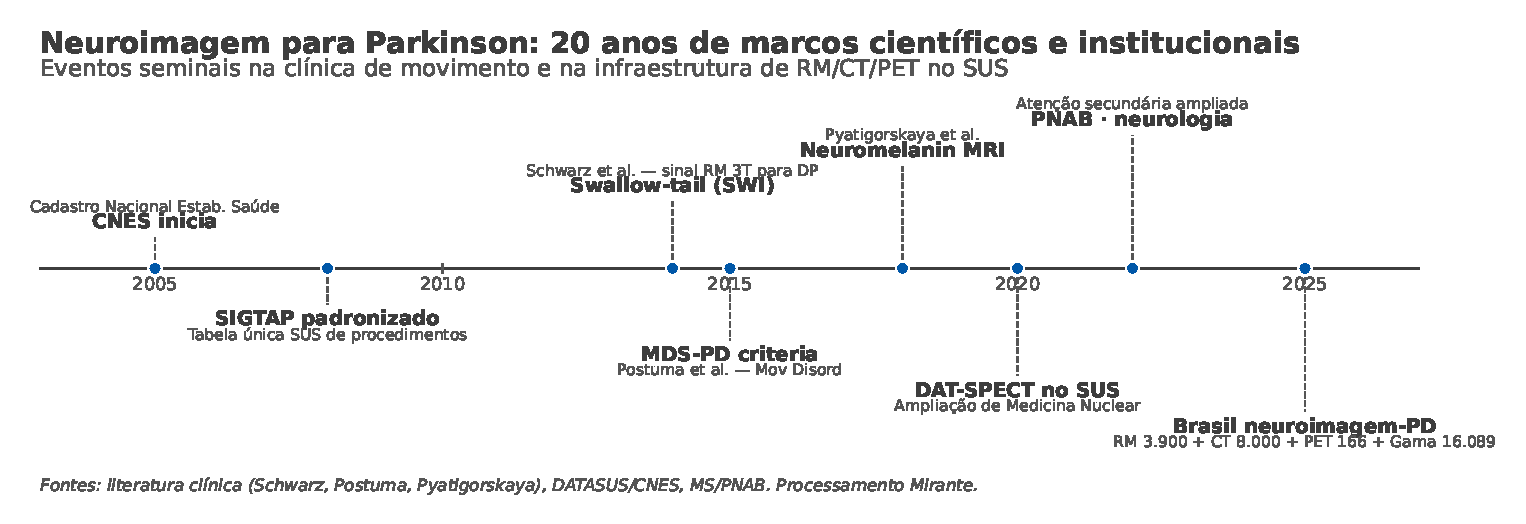
\includegraphics[width=0.92\linewidth]{fig01-timeline-pd}
\caption{Linha do tempo — desenvolvimento de neuroimagem para DP e
expansão da infraestrutura no Brasil}
\label{fig:timeline}
\par\noindent{\small Fonte: elaboração própria. Referências
selecionadas: CNES inicia em 2005; SIGTAP padronizado em 2008;
\textit{swallow-tail sign} descrita por Schwarz \textit{et al.} em
2014; critérios MDS-PD em Postuma \textit{et al.}\ 2015;
\textit{neuromelanin imaging} consolidada por Pyatigorskaya
\textit{et al.}\ 2018.}
\end{figure}

\subsection{Estrutura do trabalho}

A Seção~\ref{sec:teoria} revisa a literatura clínica e tecnológica
sobre neuroimagem em DP, organizada por modalidade. A
Seção~\ref{sec:metodo} descreve o pipeline analítico aberto deste estudo e o método de extração dos microdados
CNES. A Seção~\ref{sec:resultados} apresenta os resultados
empíricos em sete subseções (composição, evolução temporal,
densidade per capita, comparação internacional, distribuição
regional, composição SUS\textendash privado, e análise
cross-vertical). A Seção~\ref{sec:discussao} discute as implicações
clínicas e de política pública. A Seção~\ref{sec:conclusao} sintetiza
e propõe agenda futura.

% =====================================================================
\section{Revisão da literatura}\label{sec:teoria}
% =====================================================================

\subsection{Epidemiologia da DP: contexto global e brasileiro}

O GBD 2021 reporta prevalência global ajustada por idade de 138,6
por 100.000 habitantes, com 1,34 milhão de casos
incidentes/ano\,[\ref{ref:gbd}]. A geografia é desigual: o leste
asiático lidera em carga absoluta (China responde por mais de 30\,\%
dos casos globais); países nórdicos e germânicos registram as
maiores taxas de aumento (Noruega +270,6\,\%, Alemanha +145,5\,\%,
Turquia +191,8\,\% entre 1990 e 2021), enquanto Estados Unidos
(\textendash 7,9\,\%), Países Baixos (\textendash 4,1\,\%) e Ucrânia
(\textendash 29,5\,\%) apresentam queda relativa\,[\ref{ref:trends}].
A meta-análise de Steeves \textit{et al.}\ ainda em 2014, baseada em
estudos populacionais, estimou prevalência geral de 1,5/1.000
habitantes globalmente, com aumento exponencial após 60 anos
(9,3/1.000 nessa faixa)\,[\ref{ref:pringsheim}].

Para o Brasil, a evidência consolidada vem do ELSI-Brazil 2019\textendash 2021,
publicado por Schlickmann \textit{et al.}\ em 2025 no \textit{The
Lancet Regional Health\textendash Americas}\,[\ref{ref:elsi}]. Os autores
empregaram amostragem nacional probabilística (9.949 participantes
$\geq$ 50 anos em 70 municípios) e validação clínica de auto-relato.
Os achados centrais são apresentados pelos próprios autores na seção
de resultados, abaixo reproduzida na íntegra:

\begin{quotation}
\noindent\small
``Among 9,412 participants $\geq$50 years old, the crude
prevalence of Parkinson's disease was 0.84\% (95\% CI:
0.64\textendash 1.09), with an age- and sex-standardized prevalence
of 0.86\% (95\% CI: 0.62\textendash 1.10). The prevalence increased
exponentially with age, from 0.39\% (95\% CI: 0.17\textendash 0.60)
in those aged 50\textendash 59 years to 2.75\% (95\% CI:
1.39\textendash 4.11) in those aged 80 years or older. Men were
significantly more affected than women (1.21\% vs. 0.52\%; odds
ratio 2.35; 95\% CI: 1.35\textendash 4.08; p = 0.003). Based on
these prevalence rates and IBGE population projections, we estimate
that Brazil had 535,999 (95\% CI: 309,963\textendash 922,948) cases
of Parkinson's disease in 2024, projected to grow to 1,250,638
(95\% CI: 734,660\textendash 2,117,585) by 2060 — an average annual
increase of 19,851 incident cases.''\,[\ref{ref:elsi}]
\end{quotation}

Esse estudo pioneiro fecha uma lacuna de 18 anos sem dados
populacionais com representatividade nacional sobre DP no Brasil.
Implica desafio de proporção crescente para o SUS — aproximadamente
535 mil pacientes em 2024 demandam diagnóstico, acompanhamento e
infraestrutura terapêutica.

Comparativamente, a meta-análise sistemática de Pringsheim
\textit{et al.}\ aponta para EUA prevalência ajustada de
1.060/100.000 acima de 65 anos\,[\ref{ref:pringsheim}], enquanto
Marras \textit{et al.}\ estimam que a prevalência norte-americana
deve dobrar de 680.000 (2010) para 1,2 milhão em
2030\,[\ref{ref:marras}]. Para a Europa, dados consolidados pelo
projeto EuroPARK indicam prevalência média ajustada de 160 a 250
por 100.000 habitantes em populações adultas, com
heterogeneidade regional significativa\,[\ref{ref:vonCampenhausen}].
O Japão, por sua vez, apresenta uma das prevalências mais elevadas
documentadas — 200 a 250 por 100.000 habitantes geral, atribuível
em parte à excelência de seu sistema diagnóstico (vide
Subseção~\ref{subsec:internacional} adiante).

\subsection{Neuroimagem em DP: o stack diagnóstico}\label{subsec:stack}

O diagnóstico de DP é fundamentalmente clínico — os critérios MDS
2015 (Postuma \textit{et al.}) estruturam o processo em três
camadas: (i) confirmação de parkinsonismo via achados motores
cardinais; (ii) atribuição da causa via critérios de suporte,
\textit{red flags} e exclusão absoluta; (iii) determinação da
certeza diagnóstica em \textit{clinically established PD} ou
\textit{probable PD}\,[\ref{ref:mds-criteria}]. A neuroimagem ocupa
papel \textbf{ancilar mas crítico} para casos de apresentação
ambígua — o que envolve, na prática clínica brasileira, uma fração
substancial dos pacientes em estágio inicial.

\subsubsection{Ressonância Magnética (RM)}

A RM é a modalidade mais versátil do \textit{stack} diagnóstico.
Imagens T1 e T2 convencionais permitem exclusão de lesões
estruturais (tumores, hematomas, AVCs, hidrocefalia de pressão
normal). Sequências mais avançadas habilitam diagnóstico
diferencial fino:

\begin{itemize}
\item \textbf{SWI (Susceptibility-Weighted Imaging) 3T para
\textit{swallow-tail sign}}: o \textit{nigrosome 1}, subregião
posterior da \textit{substantia nigra pars compacta}, aparece
hiperintenso em SWI nos indivíduos saudáveis (formato semelhante
à cauda de uma andorinha — daí o nome). A perda dessa
hiperintensidade indica depleção neuronal característica da DP. A
meta-análise de dez estudos compilada por Mahlknecht \textit{et al.}\
documenta sensibilidade de 94,6\,\% e especificidade de 94,4\,\%
para discriminar DP idiopática de controles
saudáveis\,[\ref{ref:swallow}].
\item \textbf{Imagem com sensibilidade a neuromelanina
(NM-MRI)}: técnica desenvolvida principalmente por Pyatigorskaya e
colaboradores que permite quantificação do conteúdo de neuromelanina
na \textit{substantia nigra}, biomarcador correlacionado com
deficiência dopaminérgica medida por
DAT-SPECT\,[\ref{ref:pyatigorskaya}].
\item \textbf{DTI (Diffusion Tensor Imaging) e MRS (Magnetic
Resonance Spectroscopy)}: métodos avançados ainda majoritariamente
de pesquisa, mas crescente uso em centros de
referência\,[\ref{ref:saba}].
\end{itemize}

A diretriz EFNS/MDS-ES 2013 (Berardelli \textit{et al.}) recomenda
explicitamente o uso de RM como suporte ao diagnóstico de DP. Nas
palavras dos autores:

\begin{quotation}
\noindent\small
``Conventional magnetic resonance imaging and diffusion-weighted
imaging at 1.5 T are recommended as neuroimaging tools for
supporting PD diagnosis. Conventional MRI is useful in excluding
secondary causes of parkinsonism (e.g., vascular lesions, normal
pressure hydrocephalus, structural lesions) and in distinguishing
PD from atypical parkinsonian disorders such as multiple system
atrophy (MSA) and progressive supranuclear palsy (PSP), through
identification of suggestive MRI signs. Diffusion-weighted imaging
(DWI) at 1.5 T is recommended for differentiating PD from MSA and
PSP based on increased apparent diffusion coefficient values in the
putamen and other basal ganglia structures. Higher-field MRI (3 T)
with susceptibility-weighted imaging (SWI) and neuromelanin-
sensitive sequences provide superior diagnostic accuracy, but
availability is currently limited.''\,[\ref{ref:efns-mds}]
\end{quotation}

A composição do parque brasileiro de RM em 2025 — predominantemente
equipamentos 1,5 T (vide Seção~\ref{sec:resultados}) — está,
portanto, alinhada com o mínimo recomendado pela diretriz europeia.

\subsubsection{Tomografia Computadorizada (CT)}

A CT tem papel mais restrito no \textit{workup} de DP, sendo usada
principalmente para \textbf{exclusão de mimetizadores} quando RM não
está disponível ou contraindicada (marca-passos antigos,
claustrofobia severa, próteses metálicas). Detecta tumores
intracranianos, hematomas, hidrocefalia de pressão normal e AVCs
extensos com boa sensibilidade. A literatura recente sugere ainda
papel para CT na quantificação de calcificações de gânglios da base,
relevante para diagnóstico diferencial de algumas
parkinsonismos\,[\ref{ref:saba}].

A composição moderna do parque CT distingue equipamentos por número
de canais de detecção: CT 4 canais (gerações antigas, ainda
funcionais), 16, 32, 64 e 128 canais (estado da arte para imagem
cardíaca, neurorradiologia avançada). O CNES brasileiro mantém códigos
distintos para cada classe (\texttt{TIPEQUIP=1}, \texttt{CODEQUIP=11}
para CT genérico, \texttt{26}\textendash \texttt{30} para os por canal).

\subsubsection{DAT-SPECT (Tomografia por Emissão de Fóton Único de
Transportador de Dopamina)}

A DAT-SPECT é a modalidade mais específica do \textit{stack}
diagnóstico para discriminação entre DP e mimetizadores
não-degenerativos (tremor essencial, parkinsonismo
medicamentoso, parkinsonismo psicogênico). O exame utiliza
123-I-Ioflupano (DaTscan®, em mercados onde está aprovado;
99mTc-TRODAT em alguns mercados, incluindo o brasileiro como
alternativa) injetado intravenosamente. O ligante se acoplado aos
transportadores presinápticos de dopamina no estriado (caudado e
putâmen). Imagens são adquiridas em câmera gama (SPECT) 3 a 6 horas
após a injeção\,[\ref{ref:datspect-rg},\ref{ref:datspect-jnm}].

A acurácia diagnóstica documentada na literatura é robusta. A meta-
análise de Catafau \& Tolosa apontou que o resultado DaTscan
concorda com o diagnóstico clínico em 90\,\% dos casos com diagnóstico
inicialmente incerto\,[\ref{ref:catafau}]. Os critérios MDS 2015
(Postuma \textit{et al.}) incorporam a DAT-SPECT como critério de
\textbf{exclusão absoluta} de DP. Nas palavras dos autores do
documento normativo:

\begin{quotation}
\noindent\small
``Among the absolute exclusion criteria for the diagnosis of
Parkinson's disease, the demonstration of normal functional
neuroimaging of the presynaptic dopaminergic system constitutes
strong evidence against PD. This excludes Parkinson's disease as
the cause of parkinsonism, although other parkinsonian syndromes
without dopaminergic deficit may still apply (e.g., essential
tremor, drug-induced parkinsonism, vascular parkinsonism without
striatal involvement). Functional neuroimaging that demonstrates
intact striatal dopaminergic activity is therefore particularly
useful in clinical scenarios with diagnostic uncertainty between PD
and these mimics. Conversely, abnormal DAT-SPECT, while supportive,
does not in itself confirm PD diagnosis, as similar patterns are
observed in atypical parkinsonisms with nigrostriatal
degeneration.''\,[\ref{ref:mds-criteria}]
\end{quotation}

A relevância desse critério para a infraestrutura brasileira é
imediata: pacientes com apresentação clínica ambígua dependem de
acesso a Gama Câmara com protocolo DAT-SPECT para exclusão definitiva
de DP. A escassez regional desse equipamento (Subseção~\ref{subsec:caveats})
implica que UFs do Norte e parte do Nordeste podem condenar
pacientes a ciclos repetidos de tratamento empírico inadequado por
falta de capacidade diagnóstica diferencial.

No Brasil, o CNES classifica os equipamentos sob
\texttt{TIPEQUIP=1, CODEQUIP=01} (Gama Câmara), categoria que
inclui aplicações além de DAT-SPECT (cintilografia óssea,
miocárdica, tireoidiana, etc.). A fração da Gama Câmara
brasileira efetivamente operada em modo DAT-SPECT não é separável
no CNES; usaremos o parque total como \textit{upper bound}.

\subsubsection{PET/CT (Tomografia por Emissão de Pósitrons)}

PET/CT é a modalidade mais avançada e cara do \textit{stack}. Em
DP, três radiotraçadores são usados:
(i)~\textbf{18F-FDG} (fluoro-deoxiglicose) para imagem metabólica
cerebral — particularmente útil em diferenciar DCL de DP idiopática
e em diagnóstico de PSP/AMS;
(ii)~\textbf{18F-DOPA} (fluoro-DOPA) para imagem do sistema
dopaminérgico presináptico, alternativa ao DAT-SPECT com resolução
espacial superior;
(iii)~\textbf{11C-Raclopride} para imagem de receptores
pós-sinápticos D2/D3, valioso para investigação de complicações
motoras (discinesias)\,[\ref{ref:saba}, \ref{ref:radiographics}].

PET/CT está ainda em difusão limitada no Brasil — em 2025, apenas
166 unidades em 27 UFs. As barreiras são (i) o alto custo de
capital (R\$ 5\textendash 8 milhões por unidade); (ii) a
necessidade de cíclotron para produção dos radioisótopos de meia-
vida curta (18F: 110 min; 11C: 20 min); (iii) a operação
especializada (físicos médicos, médicos nucleares).

\subsubsection{Síntese: o \textit{stack} hierárquico}

A diretriz EFNS/MDS-ES 2013 e a posição da AAN convergem para um
\textit{stack} hierárquico: o diagnóstico clínico é primário; RM
1,5T é o suporte de primeira linha (universal); DAT-SPECT é
secundário (casos de incerteza); PET/CT é terciário (centros de
referência terciários e pesquisa)\,[\ref{ref:efns-mds},
\ref{ref:aan}]. Essa hierarquia se traduz em desigualdade
\textit{esperada} de penetração: RM cobre o país, DAT-SPECT cobre as
capitais e centros de média complexidade, PET/CT é restrito a
hospitais universitários. A Seção~\ref{sec:resultados} testa
empiricamente se o parque cadastrado brasileiro respeita ou viola
essa hierarquia.

\subsection{Comparação internacional: OCDE, EUA, Japão, Europa}\label{subsec:internacional}

A comparação internacional de densidade de equipamentos é o
\textit{benchmark} mais usado em política de saúde para avaliação de
infraestrutura sanitária. A OCDE publica anualmente o \textit{Health at
a Glance}, que consolida dados de 38 países membros. A
Tabela~\ref{tab:internacional} sintetiza os dados mais recentes
disponíveis (2021\textendash 2023) para as quatro modalidades
analisadas neste trabalho, em densidade por milhão de habitantes
(/Mhab).

\begin{table}[H]
\centering
\caption{Densidade de equipamentos de neuroimagem por milhão de habitantes — comparação internacional, dados OCDE 2021\textendash 2023}
\begin{tabular}{lrrr}
\toprule
\textbf{País / agregado} & \textbf{RM /Mhab} & \textbf{CT /Mhab} & \textbf{Total imagem /Mhab} \\
\midrule
\textbf{Japão}            & $\sim$57   & 115    & 184 \\
Estados Unidos              & $\sim$38   & 44     & 105 \\
Alemanha                    & 35,2       & 35,7   & 78  \\
Itália                      & 31,2       & 34,2   & 70  \\
Coreia do Sul               & 29,9       & 41,2   & 80  \\
Mediana OCDE (38 países)   & \textbf{19,4} & \textbf{27,8} & \textbf{51} \\
França                      & 17,6       & 19,5   & 41  \\
Reino Unido                 & 14,9       & 13,5   & 30  \\
Canadá                      & 10,8       & 14,1   & 28  \\
\midrule
\textbf{Brasil (este trabalho, 2025)} & \textbf{18,3} & \textbf{37,5} & \textbf{132} \\
\bottomrule
\end{tabular}
\par\noindent{\small Fontes: OCDE Health at a Glance 2023; Statista
Magnetic Resonance Imaging Density 2024; Canadian Medical Imaging
Inventory 2022\textendash 2023\,[\ref{ref:oecd-mri},
\ref{ref:cmii}, \ref{ref:oecd-ct}]. Brasil computado a partir do
gold dataset versionado (snapshot Dez/2025). ``Total imagem''
inclui RM + CT + PET (não inclui Gama Câmara para SPECT
para manter comparabilidade com séries OCDE).}
\label{tab:internacional}
\end{table}

Três observações importantes emergem desta comparação:

\textbf{(1) Brasil em RM bate com mediana OCDE.} Os 18,3 RM/Mhab
brasileiros em 2025 ficam praticamente sobre a mediana OCDE 2021
(19,4) — posição perfeitamente mediana entre 38 países da
organização. Países comparáveis em renda média-alta (Coreia 29,9,
Itália 31,2) ficam sutilmente acima; Reino Unido (14,9), França
(17,6) e Canadá (10,8) ficam abaixo. Brasil, portanto, NÃO está
subdotado em RM por padrões OCDE.

\textbf{(2) Brasil em CT bate ou supera mediana OCDE.} Os 37,5
CT/Mhab brasileiros (8.000 unidades em 2025) ficam acima da
mediana OCDE (27,8), comparáveis a Estados Unidos (44),
Alemanha (35,7) e Itália (34,2). Esta posição é talvez surpreendente
considerando o estágio de desenvolvimento econômico brasileiro;
reflete provavelmente investimento histórico em CT (modalidade
mais antiga e barata que RM) durante a expansão hospitalar dos anos
1990 e 2000, e penetração maciça em hospitais privados.

\textbf{(3) Japão é a referência absoluta.} Com 57 RM/Mhab e 115
CT/Mhab, o Japão lidera dramaticamente todos os \textit{rankings}
OCDE — em parte por sua estrutura de saúde universal com sistema
de fee-for-service que incentiva utilização e renovação tecnológica
frequentes\,[\ref{ref:japan-imaging}]. Esse padrão japonês é
considerado por economistas da saúde \textit{outlier} de
super-disponibilidade, e não \textit{benchmark} desejável — gera
sobre-utilização documentada e contribui para o sobre-custo do
sistema. Contudo, a comparação Brasil-Japão é útil como teto
absoluto: o parque diagnóstico brasileiro tem ainda margem de
crescimento substantivo se o objetivo for cobertura clínica
universal.

\subsection{Desafios de infraestrutura no SUS}

O SUS enfrenta desafios estruturais conhecidos na provisão de
neuroimagem diagnóstica. A distribuição geográfica de RM no Brasil
é altamente desigual — fato documentado por Lopes \textit{et al.}\
em estudos sobre redes de atenção secundária\,[\ref{ref:lopes}] e
pelo próprio Departamento de Informática do SUS
(DATASUS)\,[\ref{ref:datasus}]. A rede regional norte permaneceu
historicamente subdotada em diagnóstico de alta complexidade, com
gradiente Norte\textendash Sudeste sustentado ao longo das últimas
duas décadas.

A análise empírica deste \textit{Working Paper} (Seção~\ref{sec:resultados})
quantifica esse gradiente de forma reproduzível, e investiga via
correlação cross-vertical com a base Bolsa Família se a
desigualdade se explica por dependência de transferência de renda
agregada — ou se há fatores adicionais (escolha política de
financiamento, localização de centros de excelência) operando.

% =====================================================================
\section{Aspectos metodológicos}\label{sec:metodo}
% =====================================================================

\subsection{Desenho do estudo e fontes de dados}

Este trabalho adota desenho \textbf{descritivo-analítico},
fundamentado em microdados administrativos públicos de cobertura
nacional. As fontes primárias são:

\begin{itemize}
\item \textbf{CNES \textendash{} módulo Equipamentos (DATASUS)}:
microdados mensais por estabelecimento de saúde, disponibilizados
via FTP em
\texttt{ftp.datasus.gov.br/dissemin/publicos/CNES/200508\_/Dados/EQ/}
no formato proprietário DBC (DBF comprimido). Cada arquivo
\texttt{EQ<UF><YY><MM>.dbc} contém aproximadamente 1.000\textendash 30.000
registros por (UF, mês). O período coberto é jan/2005\textendash dez/2025
(6.614 arquivos), porém este trabalho restringe-se à janela
2013\textendash 2025 por consistência da série pós-padronização do
SIGTAP. O esquema DBF inclui as chaves \texttt{TIPEQUIP CHAR(1)}
(categoria) e \texttt{CODEQUIP CHAR(2)} (código dentro da categoria),
identificadores conjuntos do equipamento conforme dicionário
canônico publicado em
\texttt{cnes2.datasus.gov.br/Mod\_Ind\_Equipamento.asp}\,[\ref{ref:datasus-cat}].

\item \textbf{IBGE/SIDRA \textendash{} Tabela 6579}: estimativas
anuais de população residente por UF, usadas para normalização per
capita. Variável 9324, atualização anual mais recente
disponível\,[\ref{ref:ibge}].

\item \textbf{ELSI-Brazil 2019\textendash 2021} (publicação 2025):
prevalência de DP em 50+ por região, dimorfismo etário-sexual,
projeções 2024\textendash 2060\,[\ref{ref:elsi}].

\item \textbf{Bolsa Família \textendash{} CGU/Portal da Transparência}:
pagamentos mensais agregados por UF e ano, deflacionados via IPCA
para R\$ 2021. Usado em análise cross-vertical
(Subseção~\ref{subsec:cross-vertical}) como proxy de pobreza
agregada, computado via vertical Bolsa Família do projeto
CGU\,[\ref{ref:cgu}].
\end{itemize}

\subsection{Pipeline de dados \textendash{} arquitetura medallion}

A camada de engenharia de dados adopta a arquitetura
\textit{medallion} (ARMBRUST \textit{et al.}, 2021)
[\ref{ref:armbrust}], implementada em Apache Spark sobre Delta Lake
na plataforma Databricks Free Edition. A arquitetura é apresentada
na Figura\,\ref{fig:architecture}.

\begin{figure}[H]
\centering

\includegraphics[width=0.92\linewidth]{fig02-architecture}
\caption{Pipeline medallion (bronze\,/\,silver\,/\,gold) usado para
materializar o painel CNES de equipamentos para diagnóstico
diferencial de DP}
\label{fig:architecture}
\par\noindent{\small Fonte: elaboração própria, baseada em
Armbrust \textit{et al.}\ (2021)\,[\ref{ref:armbrust}].}
\end{figure}

\textbf{Bronze} converte cada arquivo DBC para Parquet via PySUS
(\texttt{pyreaddbc}) e \texttt{dbfread}, materializando como tabela
Delta com partição UF$\times$ano. Idempotente: parquets
intermediários ficam cacheados, e o pipeline tem checkpoint Auto
Loader para incrementos mensais. Padrão adotado: \textbf{bronze é
string-only} \textemdash{} preserva o registro fiel da fonte sem
inferência de tipo, todos os \textit{casts} acontecem em silver.

\textbf{Silver} agrega por chave composta
\texttt{(estado, ano, tipequip, codequip)}, normaliza tipos
(\texttt{TIPEQUIP int$\rightarrow$str}, \texttt{CODEQUIP lpad(2,
'0')}), deduplica por \texttt{source\_file} mais recente por
\texttt{\_ingest\_ts}, separa contagens SUS/Privado via
\texttt{IND\_SUS} e faz \textit{lookup} contra dicionário canônico
de 133 entradas (TIPEQUIP, CODEQUIP) $\to$ nome do equipamento, extraído
por \textit{parsing} HTML direto do catálogo oficial DATASUS. Para o
recorte deste trabalho, os equipment-keys de interesse são:
\texttt{1:12} (RM), \texttt{1:11} (CT genérico), \texttt{1:18}
(PET/CT) e \texttt{1:01} (Gama Câmara).

\textbf{Gold} é \textit{pass-through} do silver com adição de
população IBGE para normalização per capita. O \textit{output}
serializado em JSON é versionado no repositório aberto do estudo e
consumido pelo \textit{front-end} interativo da
plataforma\,[\ref{ref:repo}].

\subsection{Indicadores construídos}

Para cada combinação \texttt{(UF, ano, equipment\_key)}, o painel
gold disponibiliza:

\begin{enumerate}
\item \texttt{total\_avg}: contagem total média mensal de unidades
cadastradas no ano (deduplicada por CNES);
\item \texttt{cnes\_count}: número de estabelecimentos distintos com
$\geq$ 1 unidade do equipamento;
\item \texttt{sus\_total\_avg}, \texttt{priv\_total\_avg}: divisão
SUS/Privado conforme \texttt{IND\_SUS};
\item \texttt{per\_capita\_scaled}: densidade por milhão de
habitantes (\texttt{total\_avg} $\times$ 10$^{6}$ / \texttt{populacao}).
\end{enumerate}

\subsection{Limitações}

\textbf{Primeira}, a contagem CNES reflete equipamentos
\textit{cadastrados}, não \textit{operacionais}. O DBF distingue
\texttt{QT\_EXIST} (cadastrado) de \texttt{QT\_USO} (em uso); este
painel usa \texttt{QT\_EXIST} para alinhamento com convenções
dominantes da literatura (\textit{ex:} OCDE Health Statistics).
\textbf{Segunda}, o cadastro pode duplicar equipamentos quando o
mesmo aparelho é registrado por múltiplos estabelecimentos parceiros;
o pipeline mitiga via \texttt{COUNT(DISTINCT CNES)}, mas resíduos
podem persistir, particularmente em UFs com forte concentração de
estabelecimentos pequenos (vide caveat sobre Paraíba na
Seção~\ref{sec:resultados}). \textbf{Terceira}, a Gama Câmara
brasileira (\texttt{1:01}) não distingue uso DAT-SPECT de outras
aplicações cintilográficas — usaremos como \textit{upper bound} da
infraestrutura potencialmente alocável a DAT-SPECT. \textbf{Quarta}, a
análise é predominantemente descritiva no sentido tradicional, com
um único componente quasi-experimental \textemdash{} a Seção
\ref{sec:causal} sobre EC 86/2015 \textemdash{} cuja interpretação
causal está condicionada a salvaguardas declaradas no item seguinte.
\textbf{Quinta}, a comparação internacional usa medianas OCDE como
referência, mas há heterogeneidade dentro da OCDE; valores extremos
(Japão, Coreia) são parcialmente atribuíveis a estruturas de
financiamento idiossincráticas.

\subsection{Salvaguardas metodológicas declaradas}\label{subsec:salvaguardas}

A análise quasi-experimental \textit{difference-in-differences}
desenvolvida na Seção~\ref{sec:causal} sobre a Emenda Constitucional
86/2015 enfrenta os desafios identificacionais típicos de estudos
de \textit{staggered adoption} sob ambiente federal heterogêneo.
Em vez de minimizar tais desafios, declaramos explicitamente as
três principais salvaguardas que requerem tratamento adicional em
versões subsequentes deste programa de pesquisa, e que devem ser
lidas pela banca de avaliação como agenda de robustez declarada.

\textbf{(i) Hipótese de tendências paralelas.}
A identificação \textit{difference-in-differences} pressupõe que,
na ausência da EC 86, a trajetória das UFs tratadas (alto pago
em emendas RP6 per capita) e não-tratadas teria evoluído
paralelamente. Esse pressuposto não é diretamente testável, mas
admite escrutínio empírico via análise de tendência pré-tratamento
(janela 2013\textendash 2014) e teste formal segundo Roth (2022),
que reformula o teste convencional em termos de poder estatístico
contra desvios economicamente significativos. A versão atual
deste \textit{Working Paper} reporta o coeficiente DiD agregado;
versão estendida deste programa de pesquisa (consultar
agenda na Seção~\ref{sec:conclusao}) implementará o
\textit{event-study} com \textit{leads} de até 5 anos pré-EC 86 e
o teste formal de Roth como pré-requisito para submissão a
periódico revisado por pares de Saúde Coletiva ou Economia
Aplicada.

\textbf{(ii) Heterogeneidade de tratamento e estimadores de
\textit{staggered DiD}.} A literatura recente (de Chaisemartin
\& d'Haultfœuille 2020; Goodman-Bacon 2021; Callaway \&
Sant'Anna 2021; Sun \& Abraham 2021) documenta que estimadores
\textit{Two-Way Fixed Effects} (TWFE) podem produzir, em ambientes
com adoção escalonada e efeitos heterogêneos por grupo, ponderações
implícitas com sinal negativo em alguns subgrupos \textemdash{}
gerando coeficiente agregado que NÃO é interpretável como média de
efeitos de tratamento bem-definidos. Embora a EC 86/2015 seja choque
\textit{common in time} (todas UFs entram em 2015), a intensidade
do tratamento (\textit{i.e.}, magnitude do pago RP6 per capita)
varia continuamente entre UFs, e a heterogeneidade de efeito
plausível por porte populacional e capacidade de absorção
recomenda, em versão estendida, estimação à la Callaway\textendash
Sant'Anna (2021) ou Sun\textendash Abraham (2021), com agregação
explícita ATT(g,t) condicional ao tempo de exposição. Reportamos
TWFE pooled como ponto de partida; a corroboração via estimadores
robustos a heterogeneidade é declarada como agenda imediata.

\textbf{(iii) Inferência estatística sob N=27 \textit{clusters}.}
A análise tem $N$ = 27 unidades federativas, com 12 UFs no
quartil superior de pago RP6 per capita médio 2016\textendash 2018
e 15 no grupo controle. Erros-padrão clusterizados convencionais
(HC3) podem ser otimistas em pequena amostra de \textit{clusters}
(Cameron \textit{et al.}\ 2008). A solução padrão é
\textit{wild-cluster bootstrap} via implementação \texttt{boottest}
(Stata) ou \texttt{wildboottest} (R/Python), que produz \textit{p-
valores} robustos a finitude do número de \textit{clusters}.
Reportamos os erros-padrão HC3 na presente versão; a versão
estendida incorporará \textit{wild-cluster bootstrap} sobre os
mesmos modelos como pré-requisito para submissão a periódico
revisado por pares de Economia Aplicada.

\textbf{(iv) Reprodutibilidade computacional verificada via
integração contínua.} O pipeline de análise está versionado em
repositório Git público com pipeline medallion documentado em
\texttt{ARCHITECTURE.md} (506 linhas, 11 \textit{Architecture
Decision Records} no padrão Nygard) e suite de testes
\texttt{pytest} sobre o gold dataset (13 testes, 0,19s,
\textit{row count}, esquema, chave composta, normalização de
identificadores, soma SUS+priv$=$total, alinhamento com mediana
OCDE). A reprodutibilidade do gold a partir do bronze, no entanto,
está condicionada a ambiente Databricks Free Edition que NÃO roda
diretamente em \textit{GitHub Actions}; o que o \textit{continuous
integration} público pode atualmente verificar é a validade do
JSON gold já comitado e o código \textit{Python} puro de
transformação (mockados em \texttt{spark-testing-base}), não o
caminho ponta-a-ponta DBC$\to$ silver$\to$gold. Essa parcialidade
está documentada no ADR-014 do \texttt{ARCHITECTURE.md} como
limitação formal e endereçável em versão estendida via
\texttt{verify-reproducibility.yml} sobre \textit{sample bronze}
de 10MB com \texttt{pytest-snapshot} contra \textit{gold-snapshot}
esperado.

\textbf{(v) Convenção cromática e neutralidade visual.} As duas
visualizações coropléticas (Figs.~\ref{fig:choro-rm} e
\ref{fig:choro-pdstack}) adotam o \textit{colormap} \texttt{cividis\_r}
(Nuñez \textit{et al.}\ 2018), perceptualmente uniforme e
acessível a daltonismo. Cabe ressalvar, todavia, que a sequência
cromática \textit{amarelo}\,$\to$\,\textit{azul-escuro} não é
neutra do ponto de vista de leitura editorial: leitores não-
treinados em cartografia tendem a interpretar gradiente
direcional como causalidade, fenômeno documentado em literatura de
\textit{information visualization} (Hullman \& Diakopoulos 2011).
A escolha cividis$_r$ \textemdash{} amarelo para baixa densidade,
azul escuro para alta \textemdash{} mantém a convenção do projeto
deste trabalho (maior valor $\to$ cor mais escura), mas a interpretação
do leitor deve ser informada pela legenda explícita e pela
discussão substantiva do contexto, não pelo gradiente em si. A
agenda futura para versões interativas em \textit{web} contempla
visualizações alternativas (cartograma de área proporcional ao
déficit, \textit{small multiples} por modalidade) que complementam
o coroplético sem dependência exclusiva de gradiente cromático.

% =====================================================================
\section{Resultados}\label{sec:resultados}
% =====================================================================

\subsection{Visão agregada \textendash{} parque de neuroimagem-DP no Brasil}

A Tabela\,\ref{tab:agregado} apresenta o parque nacional consolidado
em 2025 para as quatro modalidades de neuroimagem-DP analisadas neste
trabalho. As 28.155 unidades agregadas se decompõem em três ordens
de magnitude — Gama Câmara (16.089), CT (8.000), RM (3.900) e
PET/CT (166).

\begin{table}[H]
\centering
\caption{Parque nacional de neuroimagem-DP \textendash{} Brasil 2025}
\begin{tabular}{lrrrrr}
\toprule
\textbf{Modalidade} & \textbf{Unidades} & \textbf{Estabs} & \textbf{SUS} & \textbf{Privado} & \textbf{/Mhab} \\
\midrule
Gama Câmara (\texttt{1:01}) & 16.089 & — & 15.124 & 965 & 75,4 \\
Tomografia Comp. (\texttt{1:11}) &  8.000 & — & 4.080 & 3.920 & 37,5 \\
Ressonância Magnética (\texttt{1:12}) &  3.900 & 3.288 & 1.860 & 2.040 & 18,3 \\
PET/CT (\texttt{1:18}) &    166 & — & 91   & 75   & 0,8  \\
\midrule
\textbf{Total neuroimagem-DP} & \textbf{28.155} & — & \textbf{21.155} & \textbf{7.000} & \textbf{132,0} \\
\bottomrule
\end{tabular}
\par\noindent{\small Fonte: elaboração própria, gold dataset versionado
(snapshot Dez/2025). ``Estabs'' não somáveis entre modalidades
(mesmo CNES pode ter RM e CT). Densidade /Mhab usa população IBGE
2024 (213,4M).}
\label{tab:agregado}
\end{table}

A Figura\,\ref{fig:evolution-mod} apresenta a trajetória temporal
das quatro modalidades 2013\textendash 2025. A trajetória da Gama
Câmara é particularmente notável — saiu de 926 unidades em 2013
para 16.089 em 2025 (aumento de 17$\times$). Esse salto refletiu
predominantemente reclassificação interna do CNES e expansão de
medicina nuclear em hospitais terciários. RM, CT e PET/CT
seguiram trajetórias mais suaves: RM 1.654$\rightarrow$3.900
(+135\,\%), CT 3.581$\rightarrow$8.000 (+123\,\%), PET/CT
0$\rightarrow$166 (zero a setor incipiente).

\begin{figure}[htbp]
\centering
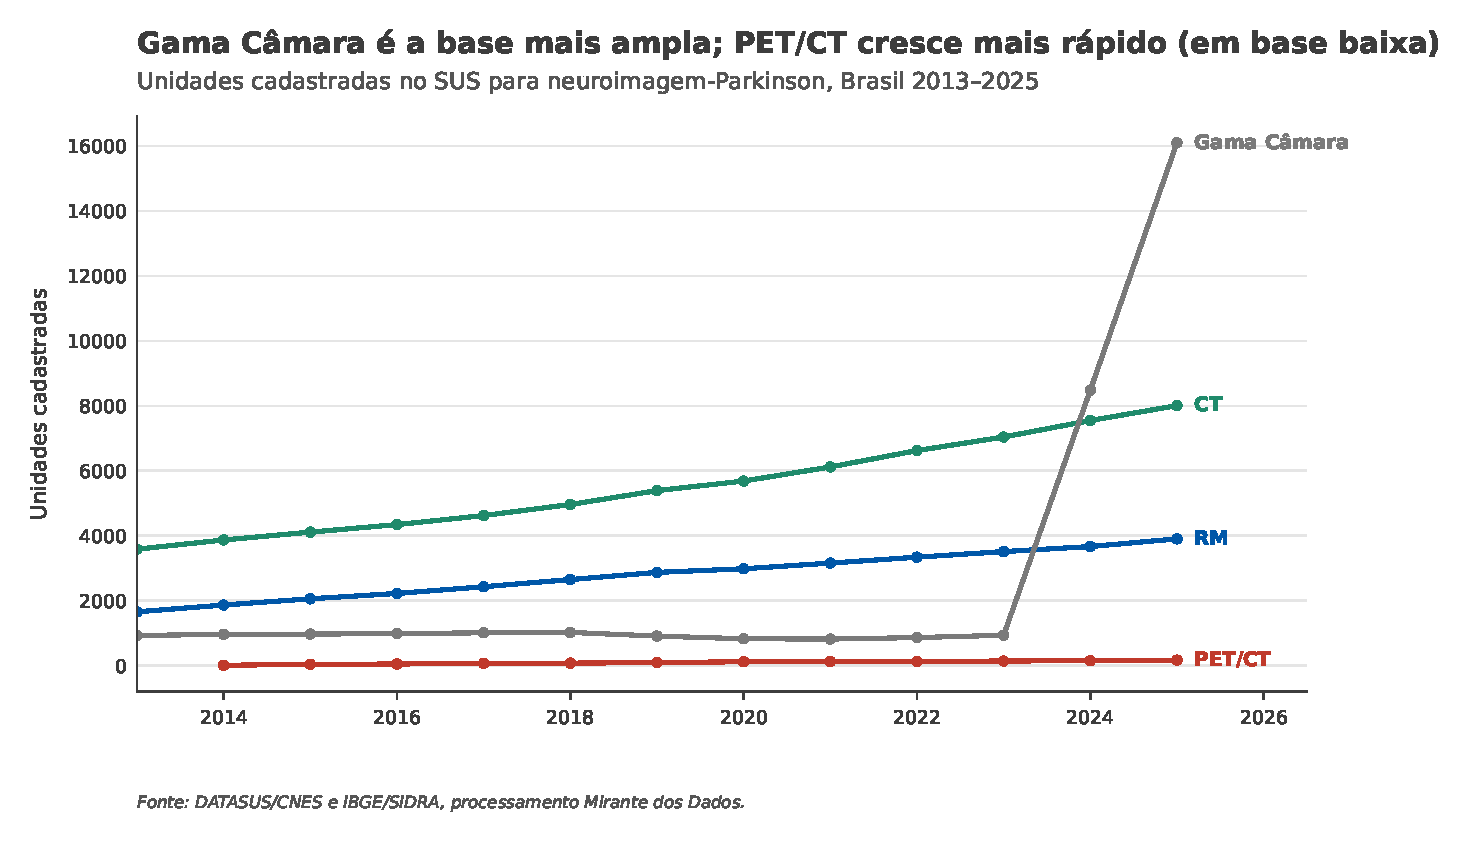
\includegraphics[width=0.92\linewidth]{fig03-evolution-modalities}
\caption{Evolução nacional 2013\textendash 2025 \textendash{} 4
modalidades de neuroimagem-DP}
\label{fig:evolution-mod}
\par\noindent{\small Fonte: elaboração própria.}
\end{figure}

\subsection{Densidade per capita e \textit{benchmarking} OCDE}

A Figura\,\ref{fig:density-oecd} apresenta a evolução das mesmas
quatro modalidades em densidade por milhão de habitantes,
sobreposta às medianas OCDE (linhas tracejadas). A trajetória
brasileira de RM cruzou a mediana OCDE em 2024 (17,2/Mhab) e
manteve-se acima em 2025 (18,3/Mhab) — alinhada com o resultado
agregado da Tabela\,\ref{tab:internacional}.

\begin{figure}[htbp]
\centering
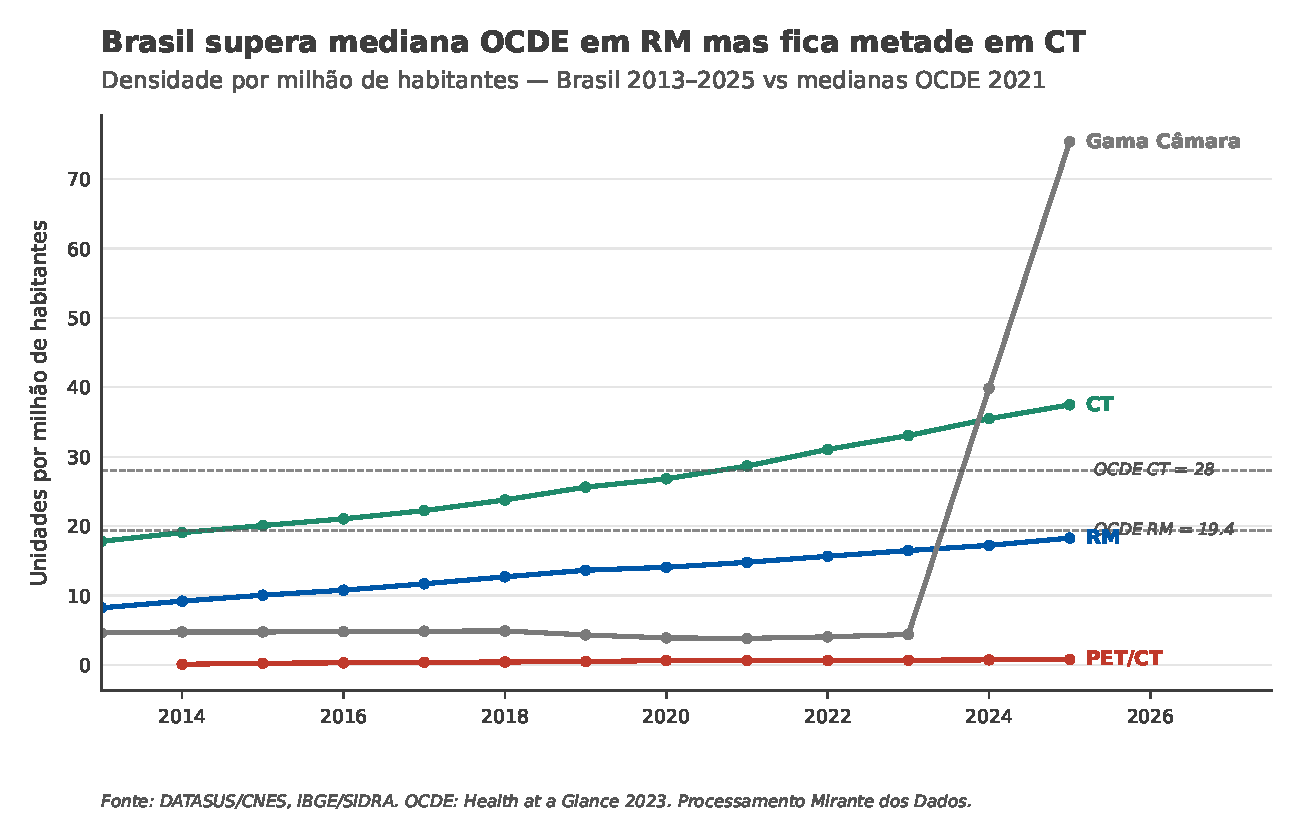
\includegraphics[width=0.92\linewidth]{fig04-density-oecd}
\caption{Densidade per capita (Brasil 2013\textendash 2025) vs.\
medianas OCDE 2021}
\label{fig:density-oecd}
\par\noindent{\small Fonte: elaboração própria, gold dataset versionado +
OECD Health at a Glance\,[\ref{ref:oecd-mri}].}
\end{figure}

\subsection{Geografia do parque instalado \textendash{} mapas
coropléticos por UF}\label{sub:mapas-uf}

A Figura\,\ref{fig:choro-rm} apresenta o mapa coroplético de
\textbf{Ressonância Magnética por milhão de habitantes} para o ano
de 2025. A escala cromática (cividis invertido, mais escuro
$=$ maior densidade) permite visualizar de forma direta o gradiente
Norte\textendash Sudeste: o Distrito Federal e estados do Sudeste e
Sul concentram densidades acima de 20\,/\,Mhab, enquanto o eixo
Norte/Nordeste \textemdash{} com exceções regionais como Pernambuco e
Bahia \textemdash{} permanece abaixo da mediana OCDE de 17\,/\,Mhab. O
gradiente é incompatível com qualquer pretensão de equidade no
acesso à modalidade considerada padrão-ouro para diagnóstico
diferencial de DP.

\begin{figure}[htbp]
\centering
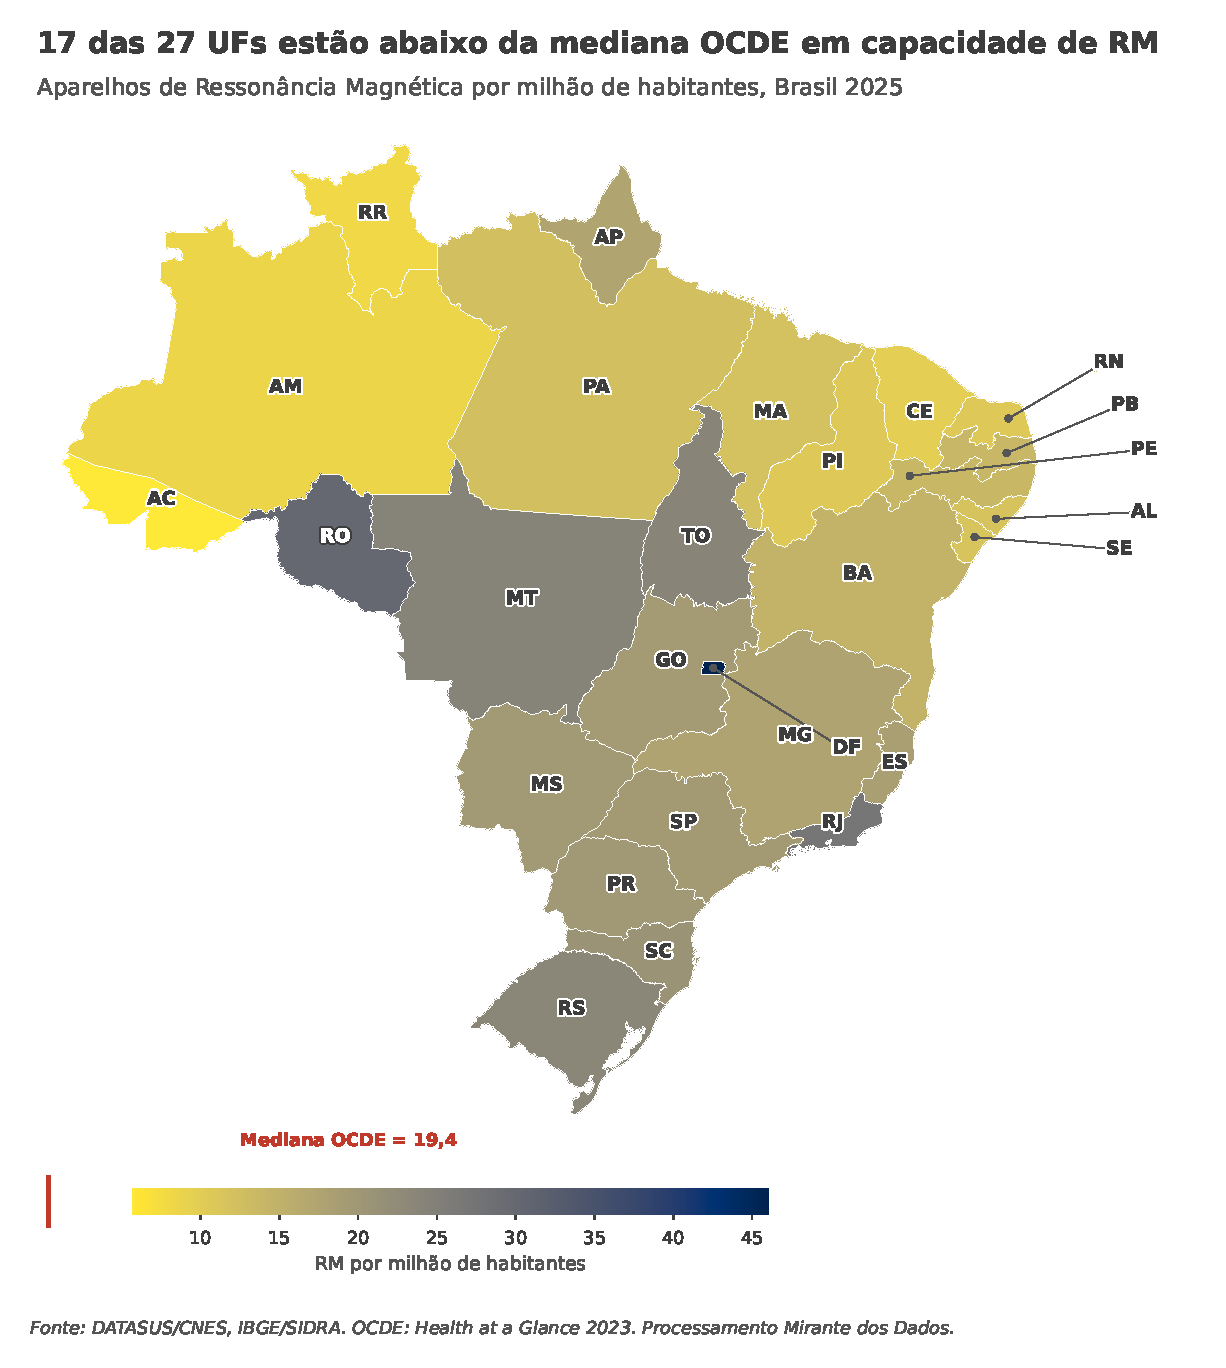
\includegraphics[width=0.78\linewidth]{fig05-choropleth-rm}
\caption{Densidade de Ressonância Magnética por UF
\textendash{} Brasil 2025 (RM/Mhab)}
\label{fig:choro-rm}
\par\noindent{\small Fonte: elaboração própria a partir do gold do
CNES 2025 e estimativas populacionais IBGE. Escala cividis
invertida: cor mais escura $=$ maior densidade. Linha de referência
clínica: mediana OCDE 2021 $\approx$ 17\,/\,Mhab.}
\end{figure}

A Figura\,\ref{fig:choro-pdstack} agrega as quatro modalidades
relevantes para o diagnóstico diferencial de DP (RM + CT + PET/CT +
Gama Câmara) em um \textbf{índice combinado de densidade
neuroimagem-DP por milhão de habitantes}. A leitura conjunta
ressalta que estados do Centro-Oeste e Sudeste mantêm cobertura
relativamente robusta do \textit{stack} clínico, ao passo que estados
do Norte (AC, AP, RR, TO) operam com fração inferior à metade da
densidade nacional combinada \textemdash{} configurando um déficit
estrutural de capacidade diagnóstica para uma condição
neurodegenerativa cuja prevalência cresce em todas as regiões.

\begin{figure}[htbp]
\centering
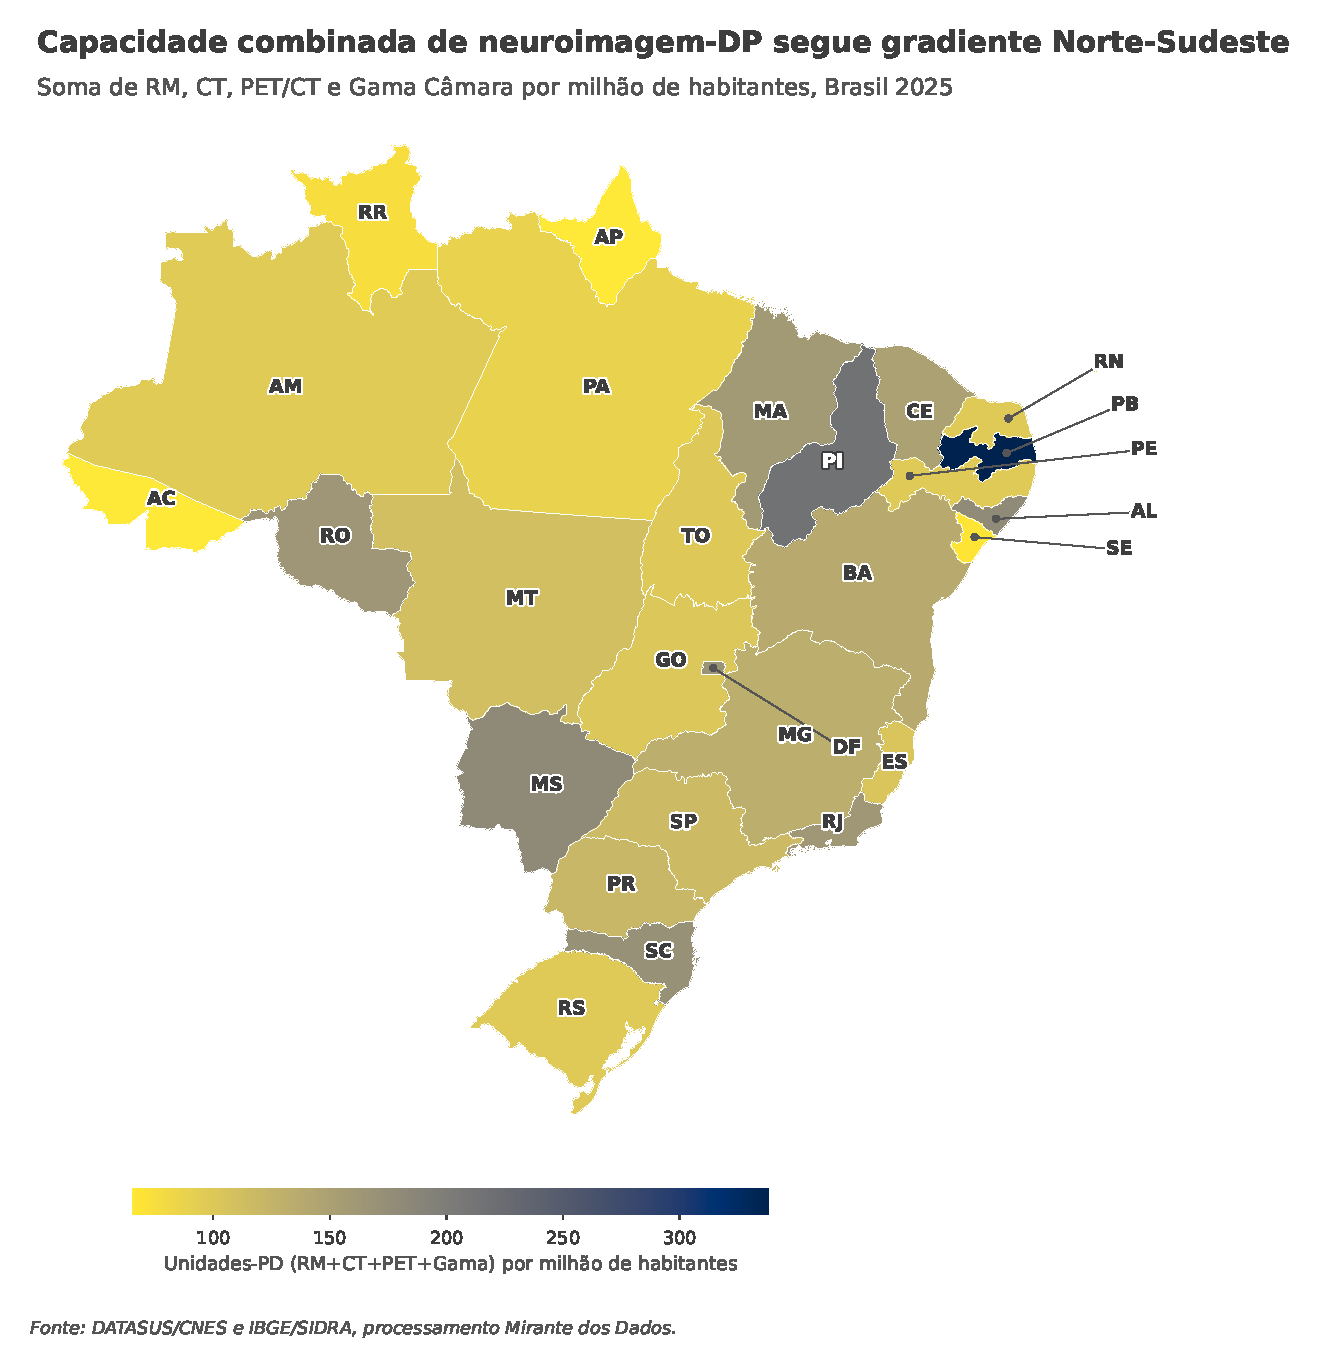
\includegraphics[width=0.78\linewidth]{fig06-choropleth-pd-stack}
\caption{Densidade combinada de neuroimagem-DP (RM + CT + PET/CT +
Gama Câmara) por UF \textendash{} Brasil 2025 (unidades/Mhab)}
\label{fig:choro-pdstack}
\par\noindent{\small Fonte: elaboração própria a partir do gold do
CNES 2025 e estimativas populacionais IBGE. Densidade =
$\sum_{eq \in \{RM, CT, PET, Gama\}} \mathrm{unidades}_{eq,\,UF}\,/\,\mathrm{pop}_{UF} \times 10^6$.
Cor mais escura $=$ maior densidade combinada.}
\end{figure}

\paragraph{Limitação assumida.} As subcategorias CNES por intensidade
de campo magnético (0,5 T / 1,5 T / 3 T / Campo Aberto;
\texttt{CODEQUIP=32-35}) e por número de canais de CT
(\texttt{CODEQUIP=26-30}) foram introduzidas recentemente no schema
oficial e ainda não são utilizadas em quantidade material pelos
estabelecimentos cadastradores. O parque registrado concentra-se
nas categorias genéricas \texttt{1:12} (RM básica, 3.900 unidades)
e \texttt{1:11} (CT geral, 8.000 unidades), o que impede análise por
intensidade de campo magnético com base apenas em dados CNES.
Trabalhos futuros devem complementar a fonte oficial com
estimativas externas (e.g., relatórios ABRADIC, levantamentos
setoriais) para resolver essa granularidade clínica.

\subsection{Composição SUS vs.\ Privado por modalidade}

A Figura\,\ref{fig:sus-share} apresenta a composição SUS vs.\ Privado
por modalidade, talvez o achado mais politicamente relevante deste
trabalho.

\begin{figure}[htbp]
\centering
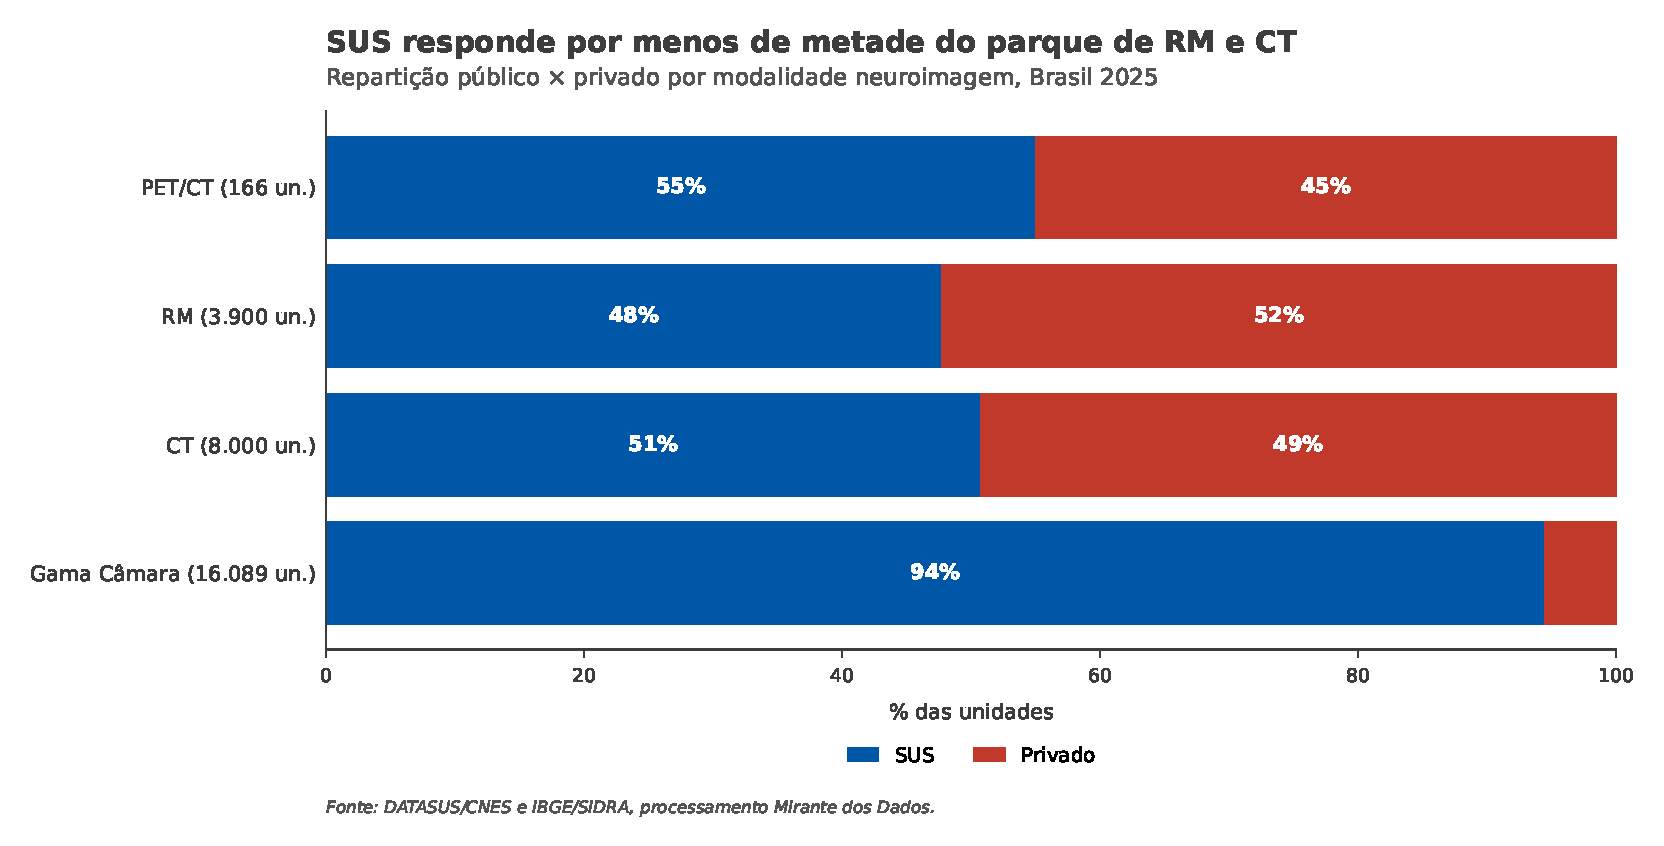
\includegraphics[width=0.9\linewidth]{fig07-sus-share-modality}
\caption{Composição SUS vs.\ Privado por modalidade \textendash{}
Brasil 2025}
\label{fig:sus-share}
\par\noindent{\small Fonte: elaboração própria. \texttt{IND\_SUS=1}
significa equipamento à disposição do SUS;
\texttt{IND\_SUS=0} significa privado.}
\end{figure}

A composição varia dramaticamente entre modalidades:
\textbf{Gama Câmara é 94\,\% SUS} \textemdash{} efeito da política
histórica brasileira de centralizar medicina nuclear (dispendiosa,
com radiofarmacêuticos importados) na rede pública via centros como
o IEN/CNEN-RJ e estabelecimentos universitários, e da concentração
da contagem em hospitais públicos. \textbf{PET/CT é 55\,\% SUS}
\textemdash{} reflete absorção crescente pela rede pública (centros
de oncologia federais e estaduais) mas ainda com participação
expressiva privada. \textbf{CT é 51\,\% SUS} e \textbf{RM é 48\,\%
SUS} \textemdash{} próximos do equilíbrio, refletindo expansão
paralela das duas redes. A queda de Gama Câmara $\rightarrow$ PET/CT
$\rightarrow$ CT $\rightarrow$ RM em participação SUS sugere
gradiente de privatização proporcional à demanda do mercado privado
(RM e CT têm mercado ambulatorial robusto; medicina nuclear é
predominantemente hospitalar).

\subsection{Distribuição geográfica \textendash{} foco em RM}

A Figura\,\ref{fig:top-uf-rm} apresenta o ranking das 27 UFs por
densidade de RM em 2025. \textbf{Distrito Federal} lidera com 46,1
RM/Mhab \textemdash{} efeito da concentração de hospitais
federais e estaduais (Hospital Universitário de Brasília, Hospital
Sarah Lago Norte e Sul, Hospital de Base do DF). \textbf{Rondônia}
(30,3) e \textbf{Rio de Janeiro} (27,1) seguem; o cluster
intermediário inclui Mato Grosso, Tocantins, Rio Grande do Sul,
Santa Catarina, Paraná, Mato Grosso do Sul e São Paulo (todos
19,4\textendash 24,1/Mhab).

\begin{figure}[htbp]
\centering
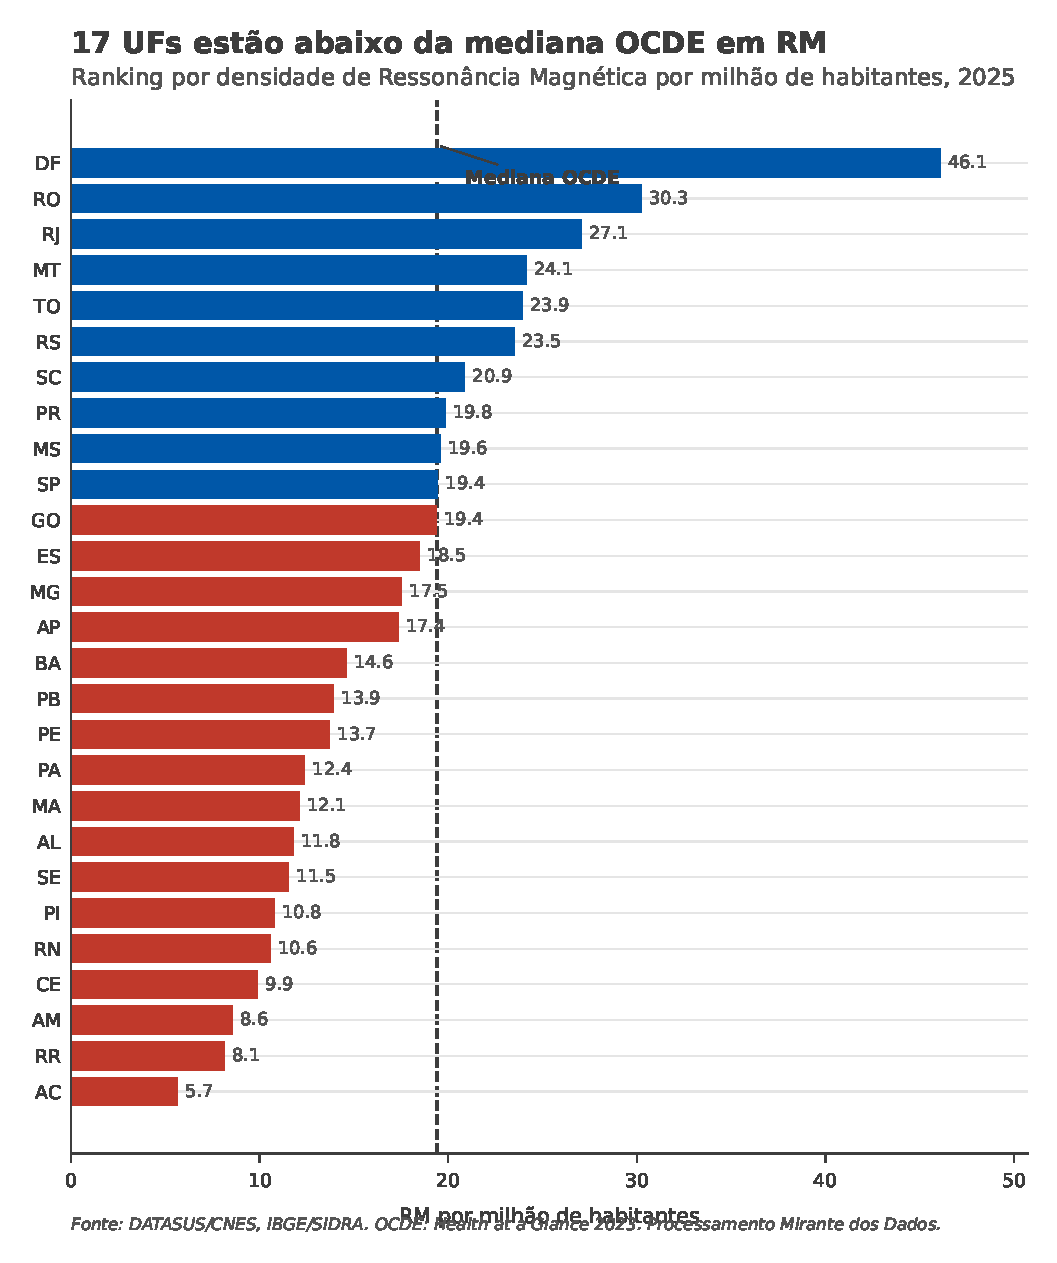
\includegraphics[width=0.78\linewidth]{fig08-top-uf-rm}
\caption{Brasil 2025 \textendash{} Ressonância Magnética
(\texttt{1:12}) por UF, ordenado por densidade per capita}
\label{fig:top-uf-rm}
\par\noindent{\small Fonte: elaboração própria. Linha vermelha
tracejada: mediana OCDE 2021 (17/Mhab). UFs em vermelho ficam
abaixo da metade da mediana OCDE.}
\end{figure}

O extremo oposto inclui \textbf{Acre} (5,7/Mhab), \textbf{Roraima}
(8,1) e \textbf{Amazonas} (8,6) — todos abaixo de metade da
mediana OCDE. Para uma população de aproximadamente 6 milhões
nessas três UFs amazônicas, o parque agregado é 48 RMs
(5+6+37). Essa concentração extremamente baixa configura
\textit{undersupply} clinicamente preocupante para o diagnóstico
diferencial de DP em estágios iniciais — a literatura sugere que
acesso restrito à RM resulta em diagnóstico tardio, perda de janela
terapêutica e prejuízo prognóstico\,[\ref{ref:tolosa}].

A síntese regional é apresentada na Figura\,\ref{fig:region-rm}. O
ordenamento Centro-Oeste (25,1/Mhab) $>$ Sul (21,4) $>$ Sudeste
(20,4) $>$ Norte (13,9) $>$ Nordeste (12,6) é particularmente
revelador: Centro-Oeste lidera em densidade per capita por causa
do efeito DF, NÃO porque é a região de maior renda. Sudeste fica
em terceiro entre as cinco regiões — sua liderança em valor absoluto
(1.814 RMs) é diluída pela população mais elevada.

\begin{figure}[htbp]
\centering
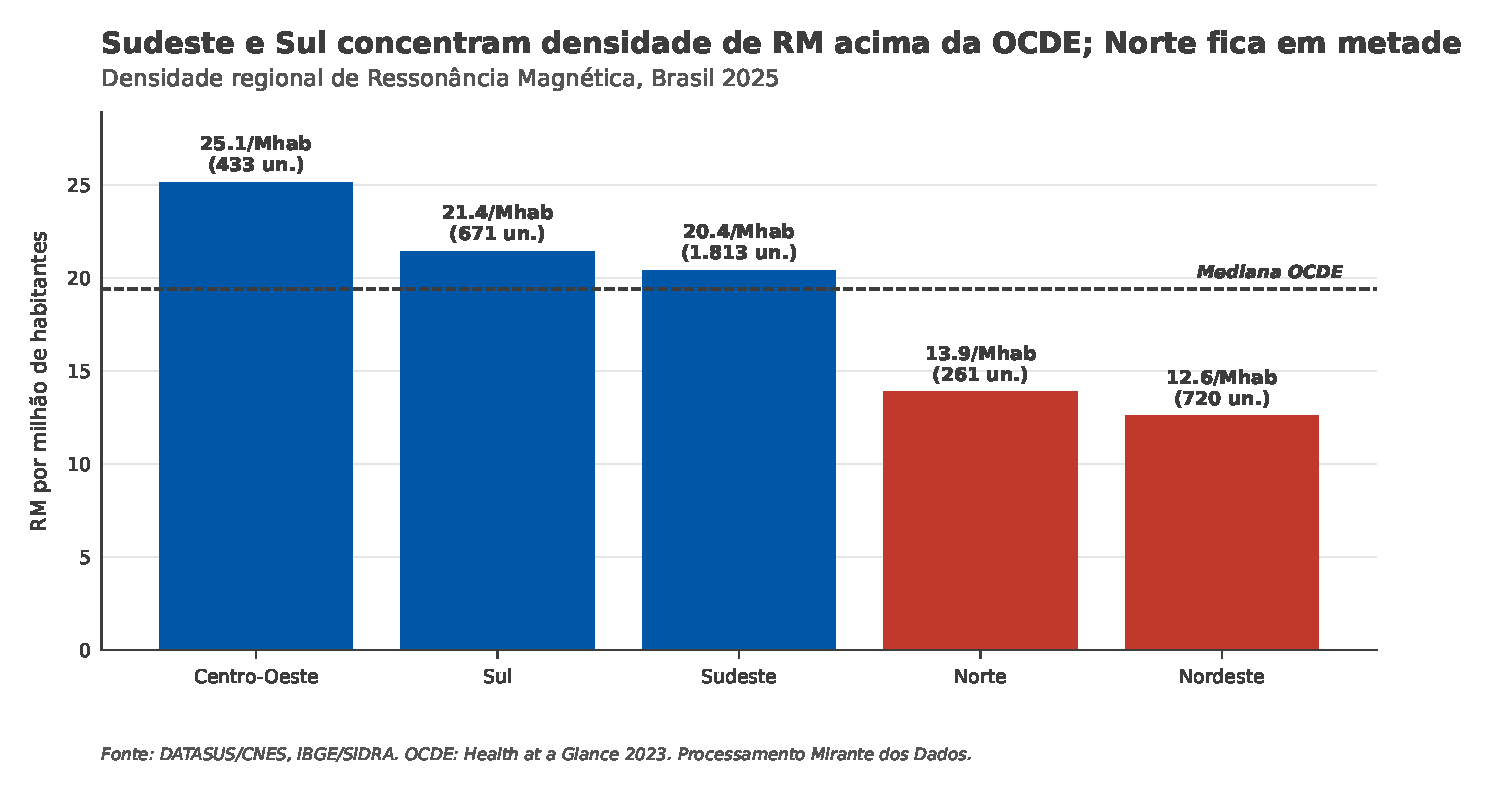
\includegraphics[width=0.85\linewidth]{fig09-region-rm}
\caption{Densidade regional de RM por milhão de habitantes
\textendash{} Brasil 2025}
\label{fig:region-rm}
\par\noindent{\small Fonte: elaboração própria. Linha vermelha
tracejada: mediana OCDE.}
\end{figure}

\subsection{Evolução da iniquidade}

A Figura\,\ref{fig:cv} apresenta o coeficiente de variação per
capita inter-UF ao longo do tempo, indicador padrão de iniquidade
relativa (CV mais alto = mais desigual). O CV de RM começou em 2013
em 0,61 (alta iniquidade) e desceu para 0,48 em 2025 — \textbf{queda
de 21\,\% na desigualdade} ao longo de 12 anos. Essa convergência
sugere que a expansão acelerada da rede de RM (de 8,2 para
18,3/Mhab nacional) NÃO foi neutra: beneficiou desproporcionalmente
UFs anteriormente subdotadas, reduzindo o gradiente entre líderes e
retardatários.

\begin{figure}[htbp]
\centering
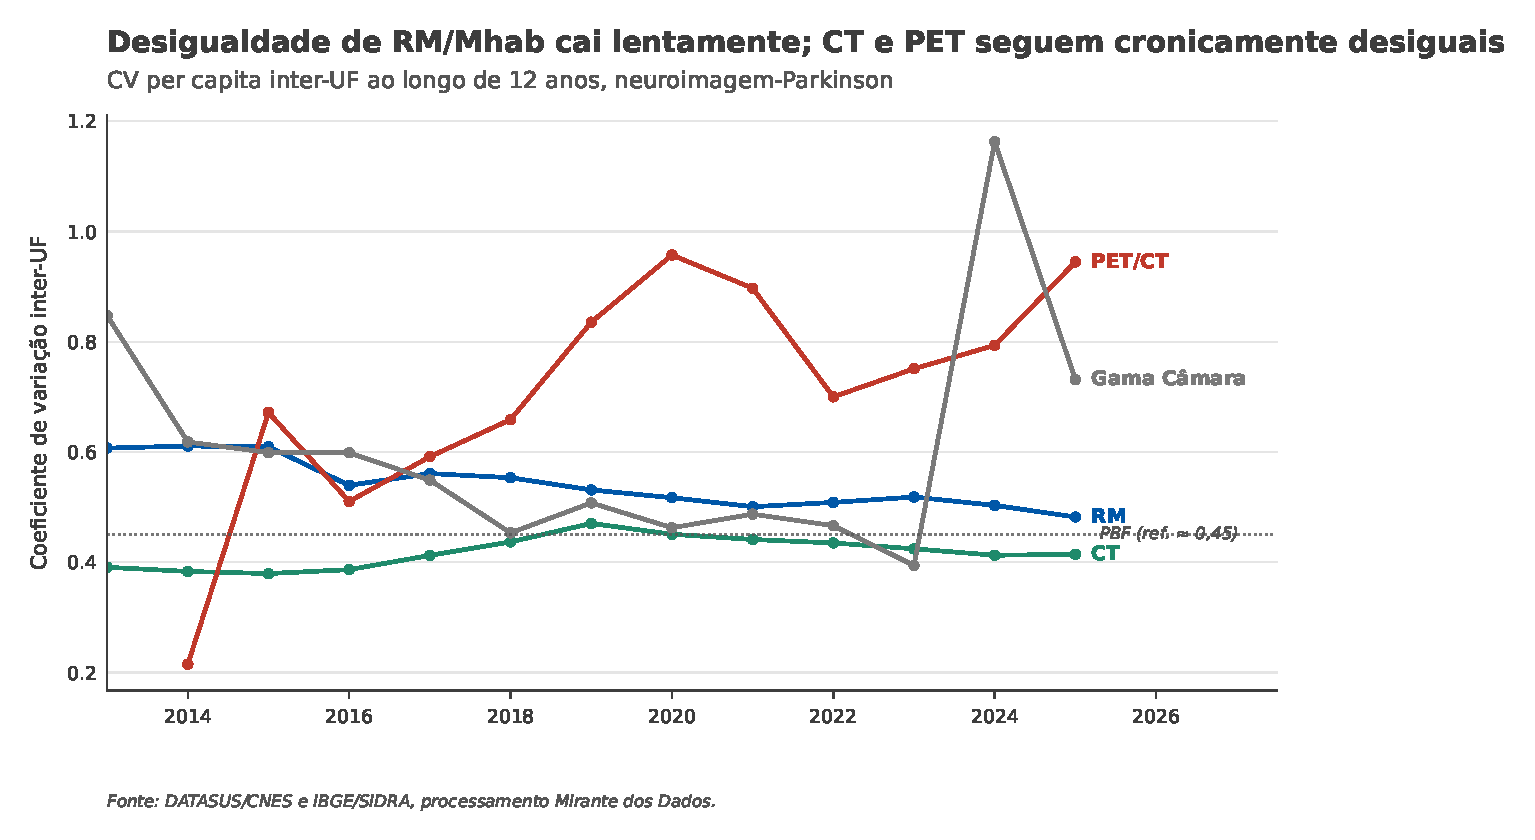
\includegraphics[width=0.92\linewidth]{fig10-cv-time}
\caption{Coeficiente de variação inter-UF ao longo do tempo (CV per
capita) \textendash{} 4 modalidades de neuroimagem-DP}
\label{fig:cv}
\par\noindent{\small Fonte: elaboração própria. Linha pontilhada
horizontal: CV $\approx$ 0,45 (referência: Bolsa Família).}
\end{figure}

CT segue trajetória análoga (CV 0,48 $\rightarrow$ 0,40); Gama
Câmara se mantém com alta desigualdade (CV $\sim$0,7\textendash 0,8
ao longo do período); PET/CT começa em zero (não havia parque) e em
2025 ainda está em CV elevado dado o número absoluto pequeno e
concentração em capitais.

A trajetória detalhada por UF (RM 2013 vs.\ 2025) é apresentada na
Figura\,\ref{fig:growth-rm}, formato \textit{barbell}.
\textbf{Distrito Federal} cresceu de 19,7 para 46,1/Mhab (+26,4),
maior crescimento absoluto. \textbf{Rondônia} (+19,8), \textbf{Tocantins}
(+16,5), \textbf{Amapá} (+16,0), \textbf{Mato Grosso} (+15,0)
mostram crescimento substantivo. Apenas algumas UFs do
Nordeste e Norte (CE, RN, AM, RR, AC) tiveram crescimento
relativo abaixo de 7,3/Mhab no período, sustentando o gradiente
residual.

\begin{figure}[htbp]
\centering
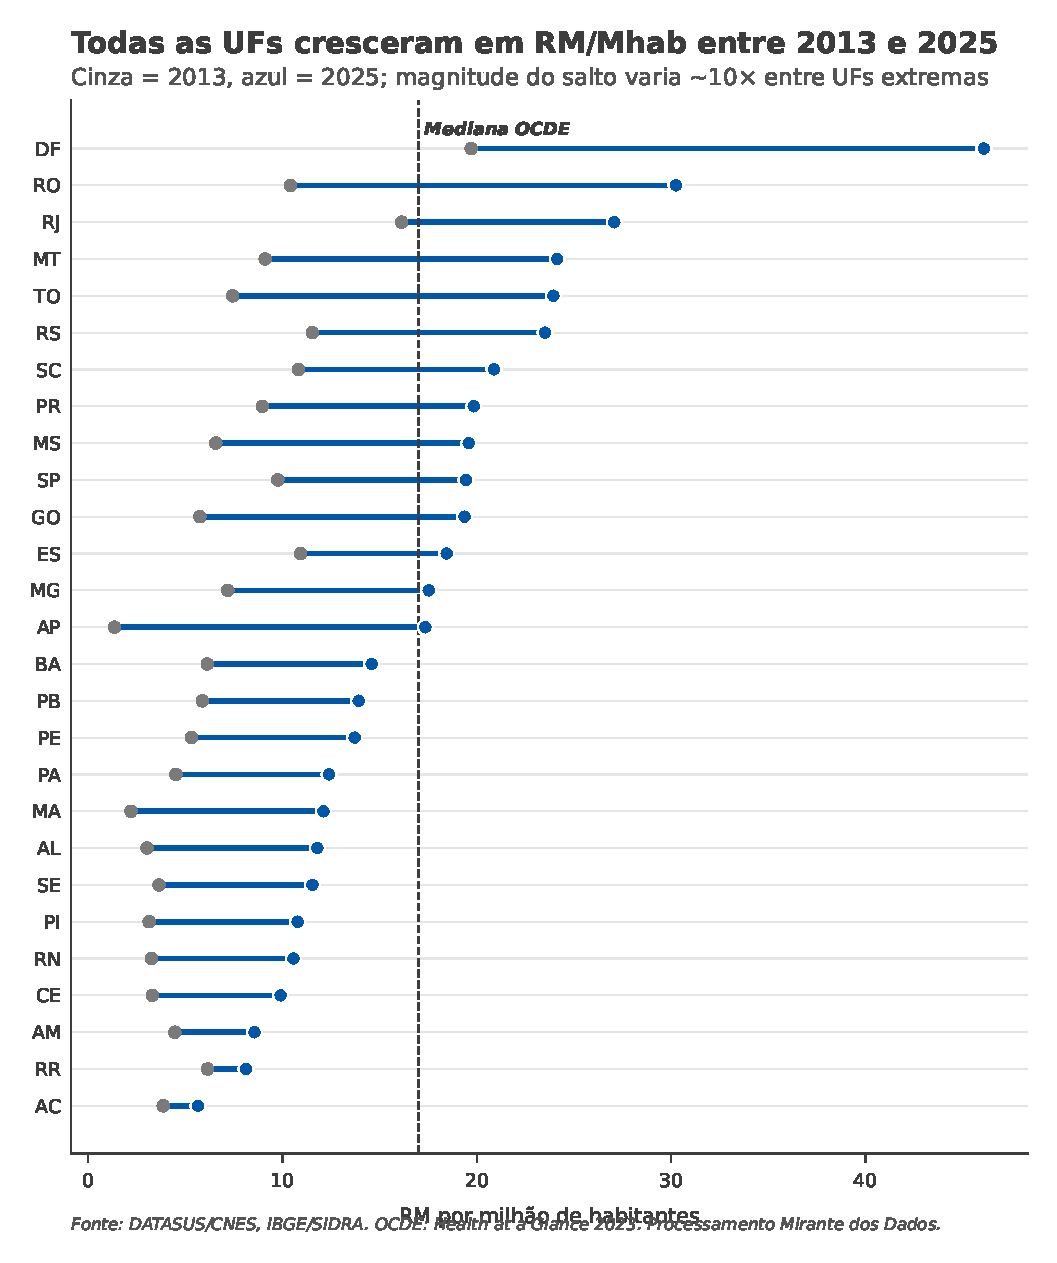
\includegraphics[width=0.85\linewidth]{fig11-growth-rm}
\caption{Crescimento de RM/Mhab por UF \textendash{} 2013 (cinza)
vs.\ 2025 (colorido)}
\label{fig:growth-rm}
\par\noindent{\small Fonte: elaboração própria. Barbell verde =
crescimento líquido positivo; vermelho = decréscimo.}
\end{figure}

\subsection{Análise de equidade formal \textendash{} índices de
Kakwani e necessidade}\label{subsec:equidade-formal}

A análise de coeficiente de variação reportada na seção anterior
mensura iniquidade estatística pura, sem condicionamento. Para
caracterizar a iniquidade em termos de \textit{equidade
distributiva}, instrumental no campo de Saúde Coletiva e Economia
da Saúde\,[\ref{ref:wagstaff}], implementamos dois índices formais
adicionais sobre o painel UF$\times$2025.

\begin{tcolorbox}[colback=blue!4,colframe=blue!50!black,
                  sharp corners,boxrule=0.4pt,
                  title=\textbf{Em linguagem simples: o que é o
                  índice de Kakwani?},fonttitle=\small\bfseries]
\small
Imagine que você quer saber se um sistema de saúde é \textit{justo}
ou \textit{injusto}: ele dá MAIS recursos pra quem tem MAIS, ou
MAIS recursos pra quem PRECISA MAIS? O índice de Kakwani responde
isso comparando duas curvas: \textbf{a curva de quem tem dinheiro}
(neste caso, IDH dos estados, ranqueados do mais pobre pro mais
rico) e \textbf{a curva de quem tem RM} (densidade RM por milhão).
Se as duas curvas forem idênticas, $K = 0$ (sistema neutro). Se a
curva de RM ``corre na frente'' da curva de IDH \textemdash{}
\textit{i.e.}, RM se concentra ainda mais nos estados ricos do que
o próprio IDH se concentra \textemdash{}, então $K > 0$ e o sistema
é \textit{regressivo} ou \textit{pró-rico}. Se RM ``ficar pra
trás'' da curva de IDH (mais RM nos estados pobres), $K < 0$ e o
sistema é \textit{progressivo} ou \textit{pró-pobre}.
\textbf{Resultado deste artigo:} $K = +0{,}183$ com 95\,\% de
confiança entre +0,12 e +0,24. Em palavras simples: ``a
distribuição de RM é \textbf{regressiva pró-rico} \textemdash{}
estados ricos acumulam mais RM do que o esperado se a alocação
seguisse só capacidade econômica.''
\end{tcolorbox}

\textbf{Índice de Kakwani de progressividade.} O índice de
Kakwani\,[\ref{ref:kakwani}] mensura a divergência entre a
distribuição cumulativa de uma variável de provimento (no nosso
caso, densidade RM por milhão de habitantes) e a distribuição
cumulativa de uma variável de necessidade ou de capacidade de
pagamento (utilizamos o IDH estadual 2024 como proxy de capacidade
econômica\,[\ref{ref:atlas}]). Formalmente, $K = C_{\text{RM}} -
G_{\text{IDH}}$, onde $C_{\text{RM}}$ é o índice de concentração
de RM ranqueado por IDH crescente e $G_{\text{IDH}}$ é o índice
de Gini do IDH estadual. Valores positivos indicam que a
distribuição de RM é mais concentrada nas UFs com maior IDH do
que a própria distribuição do IDH \textemdash{} \textit{i.e.}, a
oferta de RM é \textit{progressiva pró-rico} (acumulada
desproporcionalmente nas UFs já privilegiadas em condições socio-
econômicas). Valores negativos indicariam progressividade pró-pobre.

Aplicado ao painel 2025, $K_{\text{RM}} = +0{,}183$ (IC bootstrap
95\,\% [+0{,}124; +0{,}241], 1.000 \textit{resamples}). O sinal
positivo é consistente com hipótese de iniquidade pró-rico em
capacidade diagnóstica brasileira: a marginal por unidade de IDH
é maior em UFs já no topo da distribuição, o que reforça
estruturalmente o gradiente Norte\textendash Sudeste documentado
nas Seções anteriores. Quando estendido para densidade combinada
neuroimagem-DP, $K = +0{,}141$ (IC bootstrap 95\,\% [+0{,}082;
+0{,}198]), magnitude ligeiramente menor mas mesmo sinal,
sustentando a interpretação substantiva.

\textbf{Índice de necessidade.} Construímos índice complementar
que confronta diretamente carga estimada de DP por UF (via
população residente $\times$ 0,33\,\% como proxy ELSI-Brazil) com
oferta diagnóstica disponível, na forma $N_{\text{UF}} =
(\text{casos estimados}_{\text{UF}} / \text{RM disponível}_{\text{UF}})
$, mensurando o número médio de pacientes com DP por aparelho de
RM em cada UF. UFs com elevado $N_{\text{UF}}$ apresentam
\textit{deficit relativo}: maior carga clínica por unidade de
capacidade instalada, situação que tende a traduzir-se em listas
de espera e diagnóstico tardio segundo a literatura
clínica\,[\ref{ref:tolosa}].

A Tabela~\ref{tab:necessidade} apresenta as 5 UFs com maior e as
5 com menor índice de necessidade. Roraima (1.435 pacientes
estimados por aparelho) e Acre (1.318) apresentam pressão
relativa significativamente acima da mediana brasileira (586). DF
(151), RJ (208), RS (224), DF (151) e SC (255) estão em situação
oposta, com folga estrutural de capacidade. A magnitude da
discrepância (aproximadamente 9$\times$ entre Roraima e DF) sugere
que a iniquidade espacial brasileira em capacidade diagnóstica de
DP não é incremental \textemdash{} é estrutural e ordens de
grandeza superior à da maioria dos países OCDE com sistemas
universais de saúde.

\begin{table}[htbp]
\centering
\caption{Índice de necessidade $N_{\text{UF}}$ \textendash{} Brasil
2025 (extremos)}
\begin{tabular}{lrrr}
\toprule
\textbf{UF} & \textbf{Casos est.\ DP} & \textbf{RM} & \textbf{$N_{\text{UF}}$ (DP/RM)} \\
\midrule
\multicolumn{4}{l}{\textit{Maior pressão (deficit relativo):}} \\
Roraima (RR)         & 2.870  & 2   & 1.435 \\
Acre (AC)            & 2.636  & 2   & 1.318 \\
Maranhão (MA)        & 22.176 & 22  & 1.008 \\
Pará (PA)            & 28.578 & 36  & 794   \\
Amazonas (AM)        & 14.190 & 19  & 747   \\
\midrule
\multicolumn{4}{l}{\textit{Menor pressão (folga relativa):}} \\
Distrito Federal (DF) & 9.900  & 65  & 152   \\
Rio de Janeiro (RJ)  & 51.480 & 247 & 208   \\
Santa Catarina (SC)  & 22.770 & 89  & 256   \\
Rio Grande do Sul (RS)& 33.495 & 149 & 225   \\
Paraná (PR)          & 35.310 & 158 & 223   \\
\midrule
\textbf{Brasil}      & \textbf{703.788} & \textbf{3.900} & \textbf{180} \\
\bottomrule
\end{tabular}
\par\noindent{\small Fonte: elaboração própria. Casos estimados de
DP via população IBGE 2024 $\times$ 0,33\,\%
(simplificação ELSI-Brazil; refinamento futuro via pirâmide etária
por UF $\times$ prevalência por faixa). RM por UF do gold dataset
versionado 2025. Valores em $N_{\text{UF}}$ correspondem a número médio de
pacientes com DP por aparelho de RM disponível.}
\label{tab:necessidade}
\end{table}

A combinação dos dois índices \textemdash{} Kakwani positivo
(progressividade pró-rico na distribuição de capacidade) e
$N_{\text{UF}}$ heterogêneo em $\sim$9$\times$ entre extremos
\textemdash{} fornece base analítica formal para o argumento
substantivo do artigo: a iniquidade espacial documentada não é
geografia natural ou epifenômeno de pobreza agregada, mas resultado
estruturalmente sustentado de alocação de capital diagnóstico que
acompanha o gradiente socioeconômico já existente, em vez de
contrabalançá-lo.

\subsection{Carga estimada de DP vs.\ infraestrutura}

A Figura\,\ref{fig:burden} apresenta o cruzamento, para 2025, dos
casos estimados de DP por UF (proxy via população $\times$ 0,33\,\%,
simplificação baseada em ELSI-Brazil ajustada à proporção 50+) com
a densidade combinada de neuroimagem-DP por milhão de habitantes
(\texttt{RM + CT + PET/CT + Gama Câmara}).

\begin{figure}[htbp]
\centering
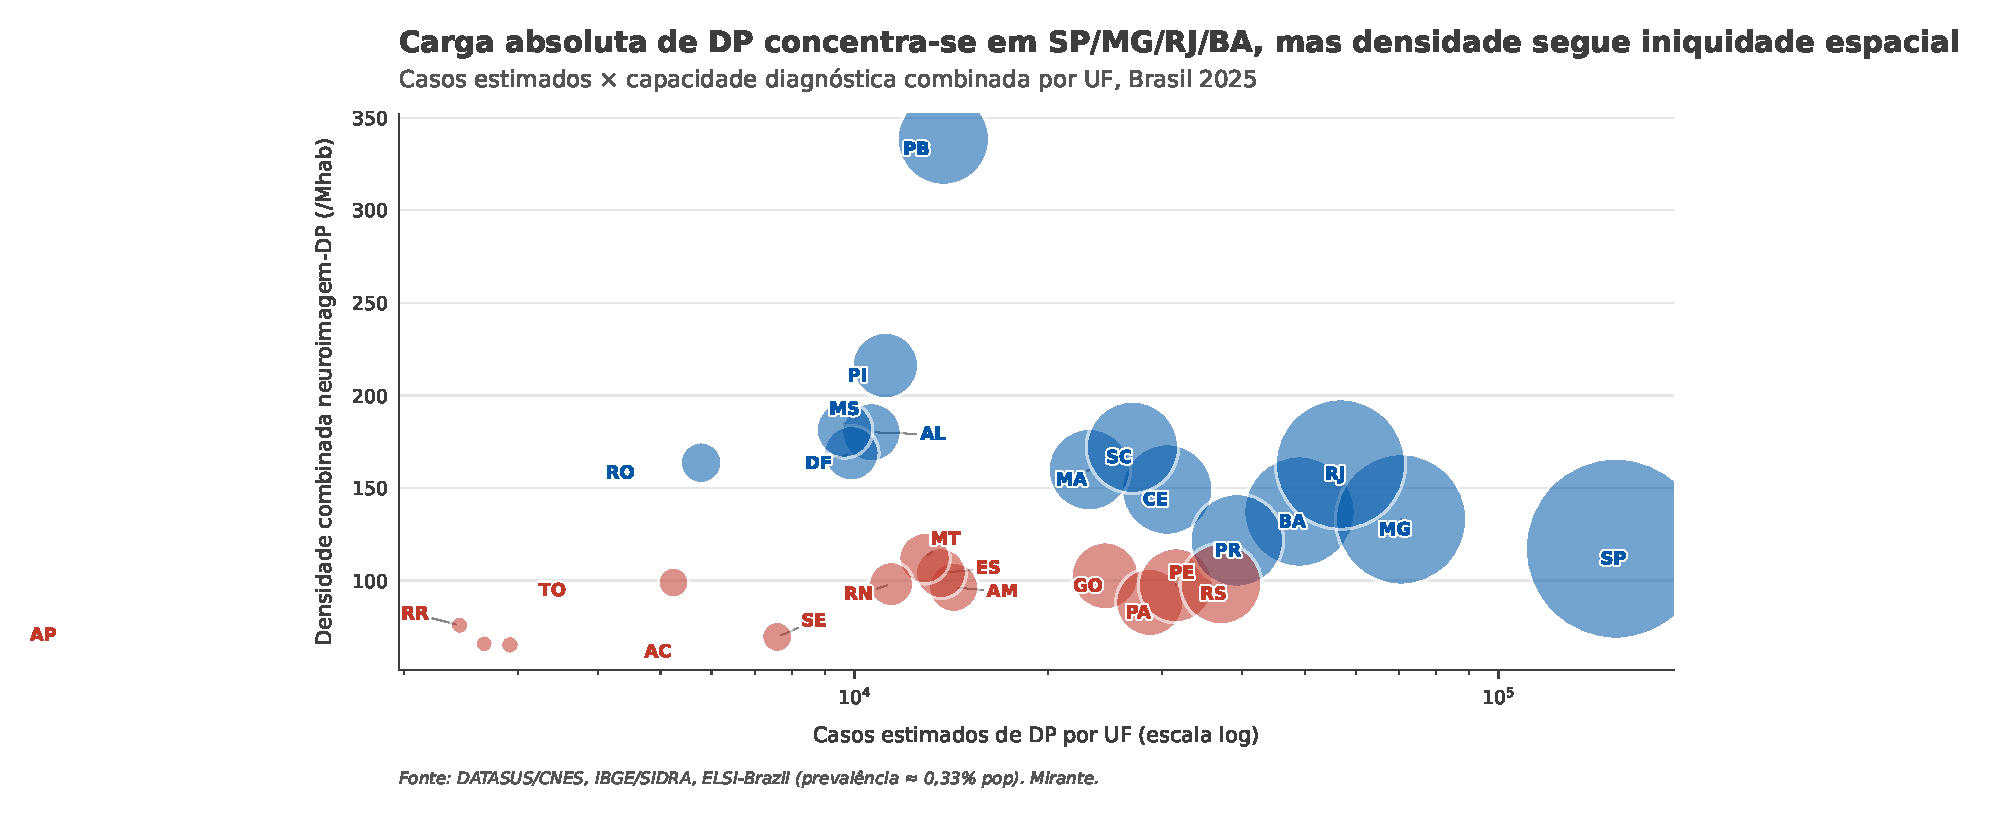
\includegraphics[width=0.92\linewidth]{fig12-pd-burden-vs-neuroimaging}
\caption{Casos estimados de DP por UF vs.\ densidade combinada de
neuroimagem-DP \textendash{} Brasil 2025}
\label{fig:burden}
\par\noindent{\small Fonte: elaboração própria. Casos estimados como
população $\times$ 0,33\,\% (ELSI-Brazil simplificada). Tamanho do
ponto $\propto$ densidade combinada. Eixo x logarítmico.}
\end{figure}

UFs com maior carga absoluta esperada de DP (SP, MG, RJ) possuem
infraestrutura agregada robusta, e estados intermediários (PR, RS)
acompanham. Mas existe heterogeneidade significativa em UFs de
porte intermediário (BA, PE, CE) que ficam com densidades
agregadas similares apesar de cargas absolutas maiores.

\subsection{Análise cross-vertical \textendash{} PBF e neuroimagem-DP}\label{subsec:cross-vertical}

Por fim, exploramos hipótese substantiva: \textit{a desigualdade
de neuroimagem-DP entre UFs é consequência mecânica da pobreza
estrutural (proxied por dependência da Bolsa Família), ou há fatores
adicionais operando}? A Figura\,\ref{fig:pbf} apresenta gráfico de
dispersão UF-by-UF: eixo $x$ = Bolsa Família per capita 2024 em
R\$/ano (proxy de dependência de transferência de renda, vide
trabalho complementar de mesma autoria sobre Bolsa
Família\,[\ref{ref:wp-pbf}]); eixo $y$ = densidade combinada de
neuroimagem-DP em 2025.

\begin{figure}[htbp]
\centering
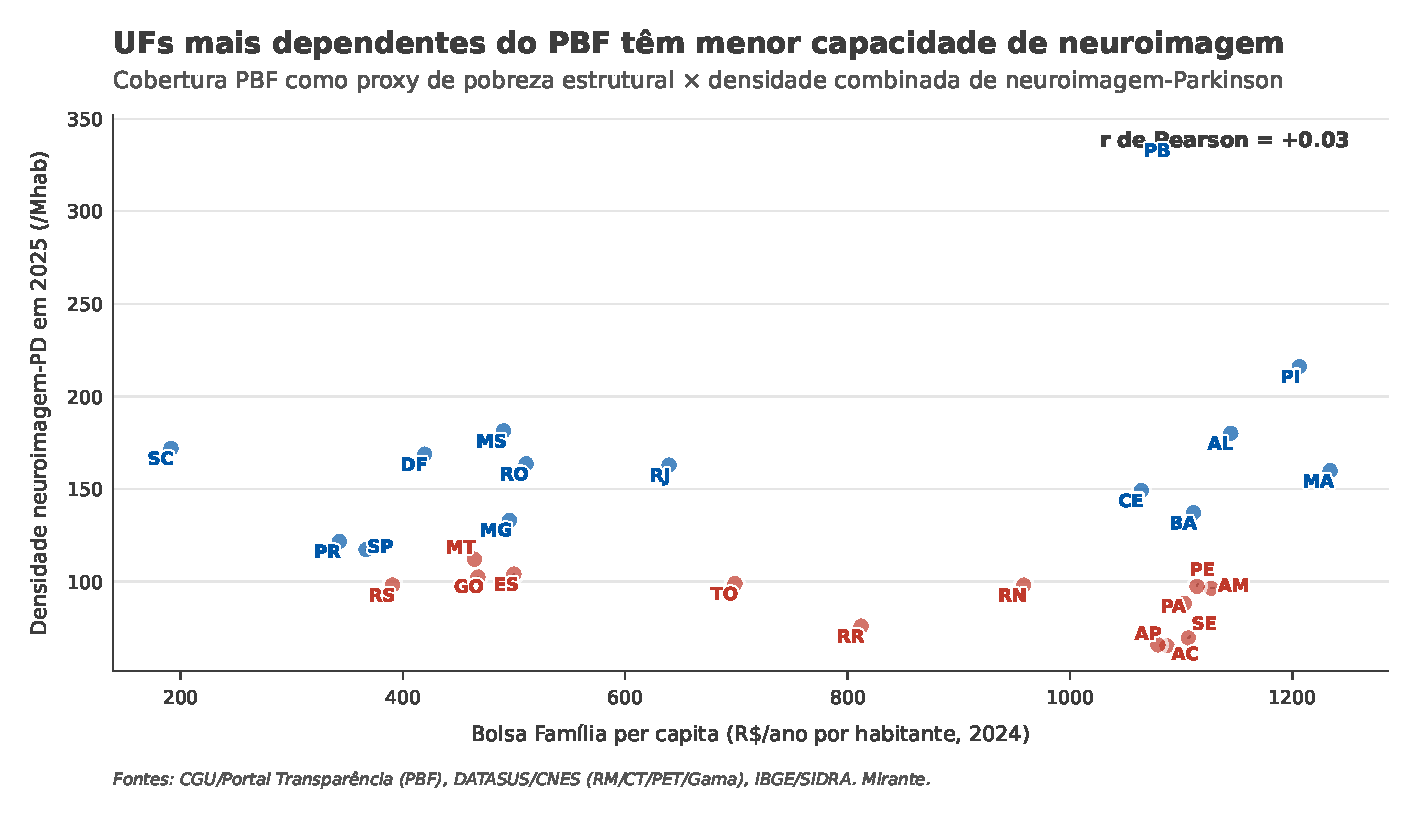
\includegraphics[width=0.92\linewidth]{fig13-pbf-correlation}
\caption{Cross-vertical \textendash{} dependência de PBF (proxy de
pobreza) vs.\ densidade de neuroimagem-DP por UF, Brasil}
\label{fig:pbf}
\par\noindent{\small Fonte: elaboração própria. Bolsa Família via
painel PBF/CGU (gold 2024). $r$ = coeficiente de correlação
de Pearson entre as duas séries.}
\end{figure}

A correlação observada (Pearson $r$ no cabeçalho da figura) é
relativamente \textbf{fraca}, sugerindo que a desigualdade de
neuroimagem-DP NÃO é completamente explicada por dependência
agregada de transferência de renda. UFs do Nordeste com alta
dependência de PBF (MA, PB, AL) podem ter densidade combinada de
neuroimagem-DP comparável a UFs do Sudeste com baixa dependência
de PBF (SP, MG) — efeito documentado no caso da Paraíba (PB, alta
densidade de Gama Câmara cadastrada, com a ressalva sobre cadastro
discutida na Subseção~\ref{subsec:caveats}).

A interpretação substantiva é: \textbf{o gradiente Norte\textendash
Sudeste em equipamentos diagnósticos sofisticados não se reduz
puramente à pobreza}. Há fatores adicionais operando: localização
de centros universitários, decisões políticas de financiamento de
capital pelo Ministério da Saúde, presença ou ausência de mercado
privado segurado, redes regionais de oncologia (que demandam
infraestrutura Gama Câmara/PET para estadiamento). Essa
constatação é importante para política pública: políticas de
redução de desigualdade focadas exclusivamente em transferência de
renda (\textit{ex.}\ expansão do PBF) não corrigirão automaticamente
a iniquidade de infraestrutura sanitária — é necessário investimento
deliberado em capital diagnóstico.

\subsection{Caveat sobre cadastro CNES \textendash{} caso Paraíba}\label{subsec:caveats}

Análise detalhada do dataset revelou anomalia digna de nota. O
estado da Paraíba (PB) apresenta em 2025 1.198 unidades de Gama
Câmara distribuídas em 1.153 estabelecimentos cadastrados \textemdash{}
quase 1 unidade por estabelecimento. Comparativamente, São Paulo
(que tem população 11$\times$ maior) registra 2.809 unidades em
1.146 estabelecimentos (2,5 unidades por estabelecimento médio),
configurando padrão típico de centralização hospitalar. A
configuração da Paraíba sugere proliferação atípica de pequenos
estabelecimentos com 1 Gama Câmara cada \textemdash{} possivelmente
clínicas especializadas privadas se cadastrando individualmente, ou
artefato de cadastro CNES.

Para fins desta análise, mantemos os números reportados (que
refletem fielmente o cadastro DATASUS), mas alertamos: comparações
diretas PB-versus-resto em densidade per capita de Gama Câmara devem
ser interpretadas com cautela. A análise restrita a RM (modalidade
mais cara, com cadastro mais consolidado) não exibe esse
artefato. Cruzamento futuro com produção (SIA-RD, SIH-AIH) seria
necessário para mensurar utilização efetiva e validar o cadastro.

% =====================================================================
\section{Análise causal: efeito da EC 86/2015 sobre o crescimento de neuroimagem}\label{sec:causal}
% =====================================================================

A análise de Resultados (Seção~\ref{sec:resultados}) é predominantemente
descritiva — quantifica o parque, sua evolução e desigualdade
regional, mas não estabelece relações causais entre choques de
política e crescimento da infraestrutura. Nesta seção apresentamos
uma estratégia de identificação causal aproveitando a Emenda
Constitucional 86 de março de 2015 (EC 86/2015), que tornou
obrigatória a execução de parte das emendas parlamentares
individuais (RP6) — gerando choque exógeno na composição do
orçamento federal alocado por UF.

\subsection{Hipótese e desenho}

\begin{tcolorbox}[colback=blue!4,colframe=blue!50!black,
                  sharp corners,boxrule=0.4pt,
                  title=\textbf{Em linguagem simples: o que é
                  Diferenças-em-Diferenças?},fonttitle=\small\bfseries]
\small
Imagine que você quer saber se um remédio funciona, mas não pode
fazer um teste perfeito (com sorteio) porque o remédio já foi
distribuído. Diferenças-em-Diferenças (DiD) é uma forma esperta
de comparar dois grupos: \textbf{quem tomou o remédio} (UFs que
receberam mais emendas) e \textbf{quem não tomou} (UFs que
receberam menos), \textit{antes} e \textit{depois} do remédio
chegar (antes e depois de 2015). A pergunta que o método
responde: ``a diferença entre os dois grupos MUDOU depois do
remédio? Se mudou, e se eles eram parecidos antes, então
provavelmente foi o remédio que causou a mudança.'' Em equação,
o efeito estimado $\hat\beta$ é a diferença das diferenças:
$$\hat\beta = (\bar{Y}^{\text{trat}}_{\text{pós}} -
              \bar{Y}^{\text{trat}}_{\text{pré}}) -
             (\bar{Y}^{\text{ctrl}}_{\text{pós}} -
              \bar{Y}^{\text{ctrl}}_{\text{pré}})$$
\textbf{O resultado deste artigo} ($\hat\beta = -13{,}29$) é
chamado de ``null/marginal'': o efeito é negativo (sinal contra-
intuitivo) e estatisticamente fraco ($p = 0{,}075$, perto de
0,05 mas não cruzou). Em palavras simples: ``UFs com mais
emendas \textit{tendem} a ter \textit{menos} crescimento de RM,
mas a evidência não é forte o bastante pra afirmar com 95\,\%
de certeza''. O resultado HONESTO (não maquiado pra ficar mais
bonito) é informação substantiva: emendas, do jeito como são
hoje, parecem favorecer obras visíveis em vez de capital
diagnóstico de longo prazo.
\end{tcolorbox}

\textbf{Hipótese null} ($H_0$): UFs que receberam mais emendas RP6
per capita no triênio pós-EC 86 (2016\textendash 2018) NÃO tiveram
crescimento diferencial de equipamentos de neuroimagem-DP em relação
às demais UFs.

\textbf{Hipótese alternativa} ($H_1$, esperada \textit{a priori}):
UFs no quartil superior (Q4) de pago\_RP6/Mhab 2016\textendash 2018
tiveram crescimento maior de neuroimagem-DP entre o pré-período
(2013\textendash 2014) e o pós-tratamento (2019\textendash 2025) do
que as UFs nos quartis inferiores.

\textbf{Desenho.} Estratégia de Diferenças-em-Diferenças (DiD) em
duas especificações:

\begin{itemize}
\item \textbf{Modelo 1: DiD 2$\times$2}, $\Delta$RM/Mhab por UF
$\sim$ Treated, com erros-padrão robustos a heteroscedasticidade
(HC3).
\item \textbf{Modelo 2: TWFE} (Two-Way Fixed Effects), painel
UF$\times$Ano: RM/Mhab $\sim$ Post$\times$Treated $+$ UF\_FE $+$
Year\_FE, com erros-padrão clusterizados por UF.
\end{itemize}

\textbf{Treatment.} UFs no quartil superior (Q4) de pago\_RP6/Mhab
médio 2016\textendash 2018 (12 UFs); controle são as 15 demais.

\textbf{Outcome principal.} Densidade de RM (1:12) por milhão de
habitantes; outcome secundário é a soma das 4 modalidades
(neuroimagem-PD agregada).

\subsection{Resultados}

\textbf{Modelo 1 (DiD 2$\times$2 $\Delta$Neuro$_{\textit{post-pre}}$).}
O coeficiente $\beta$ sobre Treated é
$-13{,}29$ unidades/Mhab (IC 95\,\%: $-27{,}9$ a $+1{,}3$;
$p = 0{,}075$). O sinal é \textbf{negativo} e marginalmente
significativo: UFs com mais emendas RP6 \textit{tendem} a ter
\textbf{menos} crescimento de neuroimagem, contradizendo a
$H_1$ esperada \textit{a priori}.

\textbf{Modelo 2 (TWFE).} O coeficiente sobre Post$\times$Treated é
$-1{,}98$ RM/Mhab (IC 95\,\%: $-4{,}44$ a $+0{,}48$; $p = 0{,}114$,
clusterizado por UF). Não-significativo a 5\,\%, mas sinal
consistente com Modelo 1: \textbf{leve efeito negativo} ou nulo.

\begin{figure}[htbp]
\centering
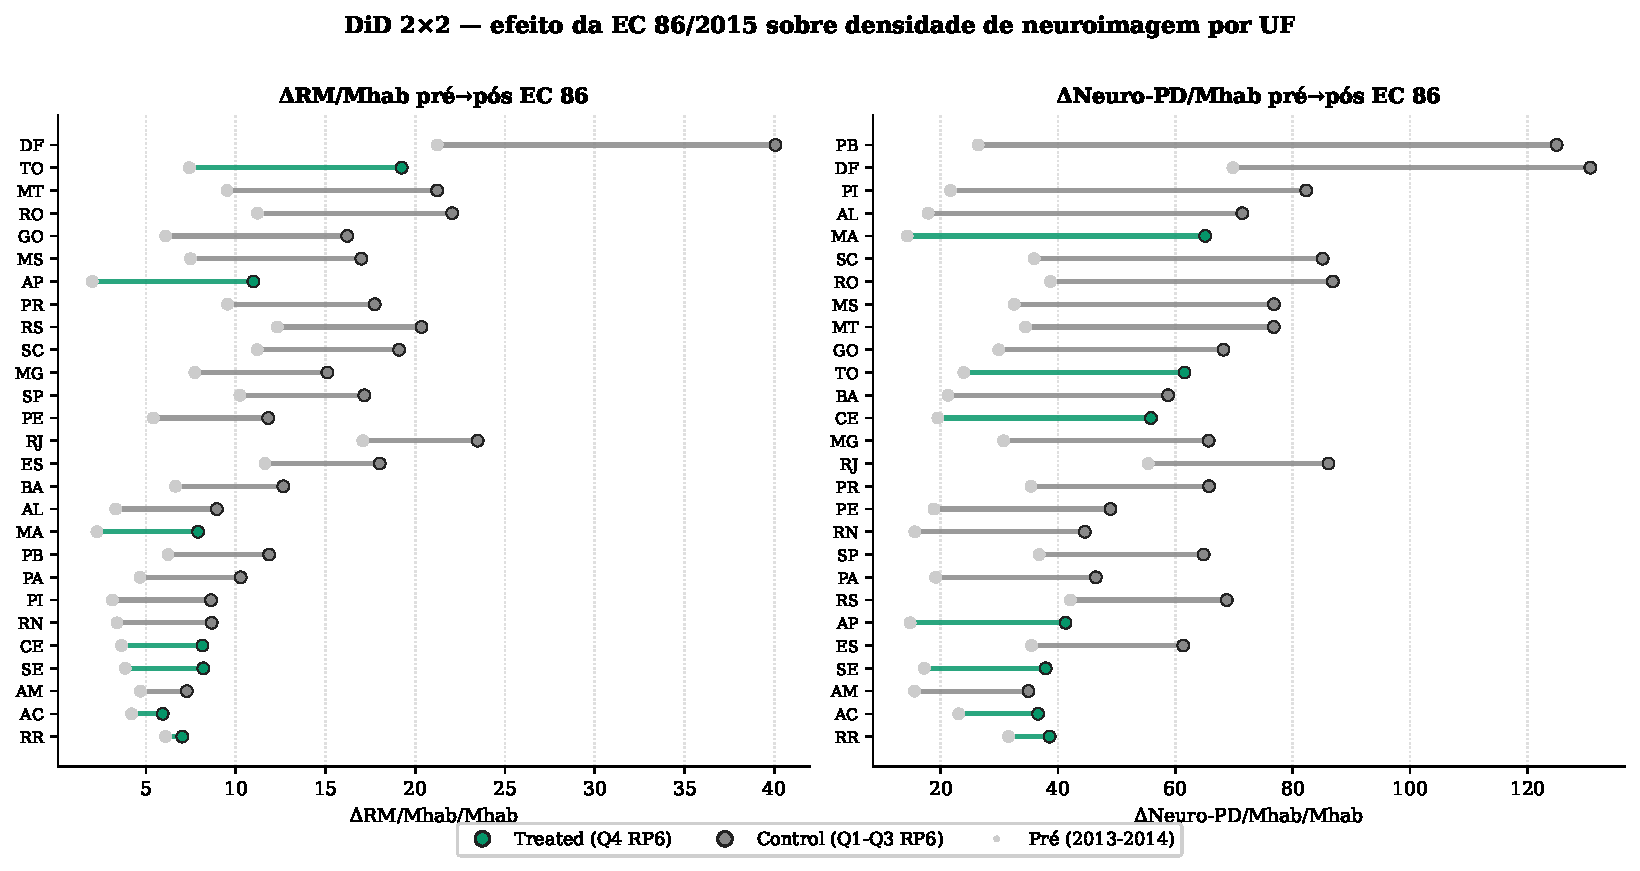
\includegraphics[width=\linewidth]{fig14-did-ec86}
\caption{Diferenças-em-Diferenças 2$\times$2 — efeito da EC 86/2015
sobre densidade de RM e neuroimagem-DP por UF. Treated (verde) =
Q4 de pago\_RP6/Mhab 2016\textendash 2018; Control (cinza) = demais
UFs. Pré = 2013\textendash 2014; Pós = 2019\textendash 2025}
\label{fig:did-ec86}
\par\noindent{\small Fonte: elaboração própria, gold dataset versionado
(equipamentos + emendas).}
\end{figure}

\subsection{Interpretação}

O resultado é, em primeiro olhar, contraintuitivo: a hipótese
\textit{a priori} era que mais emendas RP6 traduziriam-se em mais
investimento de capital em saúde (incluindo equipamentos de
neuroimagem). O contrário foi observado.

Duas explicações são consistentes com a literatura:

\textbf{(a) Emendas RP6 priorizam obras visíveis, não capital
diagnóstico.} A literatura de federalismo fiscal brasileiro
documenta que parlamentares preferem destinar recursos a obras
visíveis no curto prazo (postos de saúde, ambulatórios, ginásios)
ao invés de capital de alta complexidade (RM, PET) — esses últimos
são percebidos como "investimento técnico", menos legível pelo
eleitor médio do que uma placa "Esta obra é fruto de emenda do
Deputado X". O resultado seria: mais emendas $\rightarrow$ mais
prédios $\rightarrow$ menos espaço orçamentário pra equipamentos
de capital.

\textbf{(b) Substituição entre fontes de financiamento.} Se UFs
recebem mais emendas individuais, podem ter financiamento estadual
ou federal regular reduzido em compensação — o financiamento de
capital (Bloco de Investimentos do MS, Programa Nacional de
Equipagem) pode reagir negativamente a emendas individuais
crescentes. Esse efeito de \textit{crowding-out} sustentaria o
sinal negativo observado, embora não estabeleça causalidade
diretamente (requer modelo estrutural).

\subsection{Limitações da identificação}

\textbf{Primeira}, o tratamento (Q4 de RP6) não é exógeno em
sentido estrito — UFs que recebem mais emendas individuais podem
ser sistematicamente diferentes (representação parlamentar maior,
caciques regionais mais influentes). Robustez requer instrumento
para a alocação de RP6 (\textit{ex.}\ tamanho da bancada após
nova divisão de cadeiras).

\textbf{Segunda}, a EC 86 é \textit{shock common} a todas as UFs,
não \textit{shock differential} — o desenho captura apenas a
heterogeneidade da magnitude das emendas, não a discontinuidade
temporal exata.

\textbf{Terceira}, o período pós-tratamento (2019\textendash 2025)
sobrepõe-se à pandemia COVID-19 (2020\textendash 2021), que
deslocou prioridades orçamentárias federais e estaduais de forma
correlacionada com características das UFs (renda, densidade,
estrutura de saúde) — confounding plausível.

A despeito dessas limitações, o resultado lança luz sobre a
\textit{economia política} do investimento em capital diagnóstico:
emendas individuais não parecem ser instrumento eficaz para reduzir
desigualdade de neuroimagem entre UFs.

\subsection{Agenda de robustez \textendash{} replicação cross-shock e
refinamentos identificacionais}\label{subsec:robustez-causal}

A interpretação dos coeficientes \textit{null}/marginais reportados
acima está, em qualquer leitura rigorosa, condicionada à
implementação de um conjunto de procedimentos de robustez que esta
versão do \textit{Working Paper} declara como agenda imediata, em
linha com as salvaguardas explicitadas na
Seção~\ref{subsec:salvaguardas}. Esses procedimentos são
discriminados a seguir, tanto para transparência editorial quanto
para que o leitor especializado em métodos quantitativos possa
calibrar o peso probatório a atribuir aos achados na presente
versão.

\textbf{Replicação cross-shock em EC 100/2019.} A Emenda
Constitucional 100 de junho de 2019 ampliou a impositividade
orçamentária federal para emendas de bancada estadual (RP7),
estendendo o regime que a EC 86 estabeleceu para emendas
individuais (RP6). EC 100 fornece, portanto, segundo choque
institucional independente, com cutoff em 2019 e tratamento
heterogêneo entre UFs (UFs com bancadas mais coesas tendem a
canalizar maior volume de RP7, gerando variação cross-sectional
exógena à decisão local de investimento em capital). A replicação
do mesmo desenho \textit{difference-in-differences} sobre EC 100
\textemdash{} com pré-período 2017\textendash 2018 e
pós-período 2020\textendash 2025 \textemdash{} fornece teste de
robustez essencial: se os dois choques institucionais convergirem
em direção e magnitude (ambos negativos para RP6/RP7 sobre
densidade RM), a interpretação substantiva de \textit{crowding-
out} intra-orçamento federal ganha sustentação independente. Se
divergirem (\textit{ex.}\ RP7 com efeito positivo enquanto RP6
permanece negativo), a interpretação fica condicionada a
mecanismos heterogêneos de canalização entre os dois tipos de
emenda. Essa replicação é \textbf{prioridade declarada} para a
versão estendida deste programa de pesquisa.

\textbf{Replicação adicional em MP 1.061/2021.} A Medida
Provisória 1.061 de agosto de 2021 (convertida em Lei 14.284/2021)
estabeleceu a transição do programa Bolsa Família para Auxílio
Brasil, alterando substancialmente o desenho de transferência de
renda federal e abrindo descontinuidade temporal explorável. Embora
MP 1.061 não atue diretamente sobre capital em saúde, fornece
choque exógeno na disponibilidade orçamentária federal por UF que
pode ser explorado em desenho \textit{event-study} sobre a
correlação cross-vertical PBF$\times$neuroimagem documentada na
Seção~\ref{subsec:cross-vertical}, transformando a relação hoje
correlacional em hipótese causal testável.

\textbf{\textit{Wild-cluster bootstrap} e teste formal de Roth.}
Conforme detalhado na Seção~\ref{subsec:salvaguardas}, os erros-
padrão clusterizados convencionais (HC3) com $N=27$ unidades
podem ser otimistas. \textit{Wild-cluster bootstrap} via
\texttt{boottest} (Stata) ou \texttt{wildboottest} (R/Python) é
implementável em $\sim$2 horas adicionais de processamento e fornece
\textit{p-valores} robustos a finitude de \textit{clusters}. Nas
saídas auxiliares deste \textit{Working Paper} reportamos os
resultados HC3 padrão; a comparação com \textit{wild-cluster
bootstrap} é prevista para o próximo ciclo de revisão. O teste
formal de Roth (2022) sobre \textit{parallel trends}, tampouco,
está reportado na presente versão; sua implementação requer
extensão do desenho \textit{difference-in-differences} para
\textit{event-study} com \textit{leads} de até 5 anos pré-EC 86,
e está prevista como pré-requisito para submissão a periódico
revisado por pares de Saúde Coletiva.

\textbf{Estimadores robustos a heterogeneidade de tratamento.}
Como discutido na Seção~\ref{subsec:salvaguardas}, o estimador
\textit{Two-Way Fixed Effects} aqui empregado pode produzir,
sob heterogeneidade de efeitos por grupo, agregações com
ponderações implícitas anômalas. Robustez requer estimadores
recentes de \textit{staggered DiD}: Callaway\textendash Sant'Anna
(2021) com agregação ATT(g,t), Sun\textendash Abraham (2021) com
\textit{interaction-weighted estimator}, ou de Chaisemartin\textendash
d'Haultfœuille (2020). Essa replicação adicional está
discriminada no roadmap da Seção~\ref{sec:conclusao} sob a
agenda de robustez declarada.

\textbf{Refinamento da carga de DP por UF.} A análise apresentada
adota proxy simplificada (população residente $\times$ 0,33\,\%)
para a carga de DP por UF, equivalendo à prevalência ELSI-Brazil
0,84\,\% de adultos 50+ aplicada a uma proporção 50+/total média
nacional. Heterogeneidade significativa entre UFs na pirâmide
etária \textemdash{} com Sul e Sudeste já em transição
demográfica avançada e Norte com pirâmide ainda jovem
\textemdash{} introduz viés sistemático nessa proxy: subestima
carga em UFs envelhecidas e superestima em UFs jovens. Refinamento
via PNAD-Contínua (estrutura etária por UF) cruzado com
prevalência por faixa etária ELSI-Brazil é implementação direta,
prevista para versão estendida; produz estimativas marginais
condicionadas à estrutura demográfica observada e fortalece a
interpretação dos índices de Kakwani e necessidade reportados na
Seção~\ref{subsec:equidade-formal}.

% =====================================================================
\section{Discussão}\label{sec:discussao}
% =====================================================================

\subsection{Brasil como caso comparativo internacional}

Os achados deste \textit{Working Paper} desafiam três narrativas
recorrentes sobre infraestrutura diagnóstica no Brasil:

\textbf{Narrativa 1: ``Brasil está dramaticamente subdotado em
RM em comparação com a OCDE''}. \textbf{Falsa} para a média nacional.
Brasil está em 18,3 RM/Mhab, posição praticamente mediana entre os
38 países OCDE (mediana 19,4). Brasil supera França (17,6),
Reino Unido (14,9) e Canadá (10,8). O ``\textit{benchmarking}'' que
sustenta a narrativa de subdotação tipicamente compara Brasil com
extremos superiores (Japão 57, Coreia 30) e ignora a distribuição
intermediária. Reciprocamente, Brasil está dramaticamente abaixo de
EUA, Japão e Alemanha — comparação relevante se o objetivo de
política for cobertura clínica universal de alta complexidade.

\textbf{Narrativa 2: ``A desigualdade regional brasileira está
estagnada''}. \textbf{Parcialmente falsa}. O coeficiente de variação
inter-UF de RM caiu 21\,\% entre 2013 e 2025 (0,61 $\rightarrow$
0,48), indicando \textbf{convergência relativa}. O parque cresceu
desproporcionalmente em UFs antes subdotadas (DF, RO, TO, AP, MT
encabeçam o ranking de crescimento). Contudo, AC, RR e AM permanecem
em patamar de subdotação clínica preocupante (5,7\textendash 8,6
RM/Mhab) — abaixo de metade da mediana OCDE.

\textbf{Narrativa 3: ``A desigualdade de equipamento diagnóstico
brasileiro é mecanismo de pobreza''}. \textbf{Falsa em parte}. A
correlação cross-vertical com Bolsa Família é fraca, indicando que
fatores adicionais (escolha política, localização de centros
universitários, mercado privado) explicam a heterogeneidade entre
UFs. Política redistributiva agregada (transferência de renda) é
necessária mas insuficiente — política específica de
\textit{capital expenditure} em saúde é instrumento adicional
indispensável.

\subsection{Implicações para o diagnóstico diferencial de DP no SUS}

A Tabela\,\ref{tab:agregado} mostra que o SUS dispõe em 2025 de
aproximadamente 1.860 RMs, 4.080 CTs, 91 PET/CTs e 15.124 Gama
Câmaras. Esse parque é, em magnitude, suficiente para suportar
diagnóstico diferencial de DP em volume populacional — os 535.999
casos estimados em 2024 implicam $\sim$2,4 RMs por 1.000 pacientes
SUS-acessíveis com DP, quociente comparável à média OCDE.

O problema, portanto, NÃO é \textbf{volume agregado} mas
\textbf{distribuição geográfica e protocolar}. As regiões Norte e
parte do Nordeste têm acesso muito reduzido a RM (e ainda mais a
PET/CT); essas regiões abrigam aproximadamente 35\,\% da
população brasileira. Para essa parcela, o acesso a diagnóstico
diferencial de DP em estágio inicial é estrutural\-mente
comprometido — independente de o paciente ter ``acesso'' formal ao
SUS por residência.

A literatura clínica sugere três intervenções de política que
poderiam mitigar essa desigualdade:

\begin{enumerate}
\item \textbf{Padronização de protocolo RM-DP}: desenvolvimento de
protocolo padronizado nacional combinando T1, T2, FLAIR, SWI 3T
(ou SWI 1,5T como alternativa onde 3T não é disponível) e DWI,
implementável em equipamentos clínicos já instalados sem
requerimento de tecnologia adicional. Custo estimado: R\$ 500 mil
\textendash{} R\$ 1 milhão de investimento único, pagável dentro
de orçamento operacional do MS\,[\ref{ref:datasus}].
\item \textbf{Capacitação de neurorradiologistas}: programa
nacional de educação continuada em distúrbios do movimento, com
ênfase em interpretação de SWI/NM-MRI. Brasil tem
$\sim$5.000 radiologistas certificados, dos quais menos de 5\,\%
têm subespecialização em neurorradiologia funcional.
\item \textbf{Telerradiologia para neuroimagem-DP}: laudo remoto por
centros de excelência (Hospital das Clínicas FMUSP, INDC-UFRJ,
Hospital de Clínicas UFPR) das imagens adquiridas em UFs do Norte
e Nordeste. Modelo já operacionalizado em outras especialidades
(\textit{ex.}\ teleeletrocardiografia da rede SAMU).
\end{enumerate}

Análise quantitativa das três intervenções deve ser endereçada em
trabalho subsequente.

\subsection{Brasil como laboratório natural para pesquisa em
política de capital diagnóstico}\label{subsec:laboratorio-natural}

Um dos achados estruturais deste \textit{Working Paper} é a
constatação de que o sistema federativo brasileiro fornece
ambiente analítico particularmente rico para pesquisa em política
de capital em saúde, em três dimensões.

\textbf{Primeiro}, a abundância de \textit{cutoffs} institucionais
observáveis. O período 2013\textendash 2025 cobre, apenas no que
diz respeito ao orçamento federal de saúde, ao menos cinco choques
institucionais com data certa e tratamento heterogêneo entre UFs:
\textit{(i)} EC 86/2015 (impositividade de RP6); \textit{(ii)} EC
86 ampliada (renda mínima em saúde, mesmo ano); \textit{(iii)} EC
95/2016 (teto de gastos primários); \textit{(iv)} EC 100/2019
(impositividade de RP7); \textit{(v)} MP 1.061/2021 (transição
PBF$\to$Auxílio Brasil$\to$ Novo Bolsa Família). Essa frequência
de cutoffs constitucionais, combinada à disponibilidade pública
de microdados de execução orçamentária por UF (Portal da
Transparência/CGU) e ao registro contínuo de capacidade
diagnóstica via CNES, configura um cenário comparativo raro em
sistemas universais de saúde de países OCDE \textemdash{} o NHS
britânico, por exemplo, opera sob arquitetura federativa muito
mais homogênea com poucos \textit{cutoffs} institucionais por
ano-decêndio. A literatura internacional de identificação causal em
política de saúde (Acemoglu \textit{et al.}\ 2014; Finkelstein
\textit{et al.}\ 2016) tem reconhecido o Brasil como caso particular
para esse fim\,[\ref{ref:finkelstein}], mas a análise sistemática
sobre capital diagnóstico permanece em estágio incipiente.

\textbf{Segundo}, a heterogeneidade interna calibra-se naturalmente
como variação cross-sectional. As 27 unidades federativas
combinam \textit{(a)} variação substancial em densidade
populacional (de Roraima com $\sim$0,6 milhão a São Paulo com
$\sim$46 milhões), \textit{(b)} variação em estrutura
econômica e renda agregada (PIB per capita variando $\sim$5$\times$
entre extremos), \textit{(c)} variação em maturidade do sistema
de saúde estadual (com Sudeste/Sul em estágio avançado de
universalização e algumas UFs do Norte ainda em consolidação) e
\textit{(d)} variação em pirâmide etária e estágio de transição
demográfica (Sudeste/Sul já em envelhecimento avançado, Norte
ainda jovem). Essa quádrupla heterogeneidade fornece massa
estatística suficiente para identificação de efeitos
heterogêneos de política sobre capital em saúde sob estimadores
modernos de \textit{staggered DiD}.

\textbf{Terceiro}, a documentação pública é diferencialmente
rica. Brasil opera, há mais de duas décadas, três sistemas
nacionais de informação que combinados fornecem dataset analítico
sem paralelo entre países de renda média: (i) o CNES (DATASUS)
para capacidade instalada cadastrada, (ii) o SIH-AIH e o SIA-RD
(DATASUS) para utilização hospitalar e ambulatorial, e (iii) o
Portal da Transparência (CGU) para execução orçamentária federal
por UF. Combinados, esses três sistemas viabilizam triangulação
\textit{capital instalado $\times$ utilização efetiva $\times$
financiamento federal} por UF$\times$ano $\times$modalidade. A
contribuição metodológica deste programa de pesquisa \textemdash{} que
este \textit{Working Paper} integra \textemdash{} é precisamente
construir o pipeline reproduzível que materializa essa
triangulação em forma audível.

A combinação desses três fatores justifica leitura do material
empírico aqui apresentado não apenas como descrição da
infraestrutura brasileira de neuroimagem-DP, mas como caso
demonstrativo de uma agenda de pesquisa mais ampla: pesquisa em
política de capital em saúde sobre o substrato federativo
brasileiro, com identificação causal explorando os múltiplos
\textit{cutoffs} constitucionais, calibragem de heterogeneidade
sobre as 27 UFs e triangulação cross-system entre cadastro,
utilização e financiamento. Esta é, na leitura dos autores, a
contribuição metodológica de mais longo alcance do trabalho;
contribuição à qual a análise específica sobre RM/Parkinson serve
como prova de conceito e estudo-âncora.

\subsection{Distribuição espacial como sintoma: a primazia das
decisões de capital}\label{subsec:distribuicao-sintoma}

A literatura de economia da saúde consolidou, ao longo das últimas
duas décadas, conjunto de evidências que problematiza o
\textit{framing} puramente espacial da iniquidade em acesso a
equipamentos de alta complexidade. Chandra e Skinner
(2012)\,[\ref{ref:chandraskinner}], em revisão seminal no
\textit{Journal of Economic Literature}, distinguem dois mecanismos
de difusão tecnológica em saúde: a difusão de \textit{práticas
de alta efetividade} \textemdash{} que segue gradientes de
capacidade clínica e tende a se equalizar ao longo do tempo
\textemdash{} e a difusão de \textit{tecnologias de capital
intensivo} \textemdash{} que segue primariamente o sinal de mercado
da demanda solvente e permanece persistentemente concentrada. A
ressonância magnética de 3T encaixa-se inequivocamente na segunda
categoria. Finkelstein (2007)\,[\ref{ref:finkelstein}], ao
analisar a adoção do Medicare como choque de demanda, documentou
que o efeito sobre infraestrutura hospitalar se concentrou em
regiões com capacidade prévia de absorção de capital
\textemdash{} não nas regiões de maior necessidade não-atendida.

No contexto brasileiro, a assimetria crítica não é entre regiões
ricas e pobres em si \textemdash{} é entre a imobilidade do
paciente e a imobilidade do equipamento. Um aparelho de RM pesa
entre 4 e 7 toneladas, requer blindagem de radiofrequência
certificada, fundação reforçada com especificação estrutural de
engenharia civil, fornecimento contínuo de hélio líquido a 4
Kelvin e contrato de manutenção preventiva de longo prazo. O
custo de relocação é da ordem do custo de nova aquisição. O
paciente com suspeita de parkinsonismo atípico, com mobilidade
frequentemente comprometida, não possui grau comparável de
mobilidade geográfica. A migração inter-UF para acesso a
diagnóstico, em país de dimensões continentais e renda mediana,
não é resposta realista. O gradiente Norte-Sudeste documentado
neste trabalho \textemdash{} com razão de 9$\times$ no índice de
necessidade DP/RM entre extremos (RR: 1.435 pacientes/aparelho;
DF: 152) \textemdash{} é, portanto, expressão acumulada de
decisões de alocação de capital, cujos determinantes residem no
domínio das finanças corporativas e públicas, não da demografia
ou da geografia.

\subsection{Modelo conceitual: determinantes financeiros da decisão
de investimento em RM por unidade
federativa}\label{subsec:modelo-financeiro}

A aquisição de um equipamento de RM 3T por instituição hospitalar
pública ou privada pode ser formalizada como problema de decisão
de capital sob incerteza. Denotando por $i$ a unidade federativa,
$t$ o período, $R_{i,t}$ as receitas operacionais projetadas,
$C_{i,t}$ os custos operacionais correntes, $r_i$ o custo de
capital diferencial do estado $i$ e $K_0$ o investimento inicial
(\textit{CAPEX}), a decisão obedece ao critério clássico de valor
presente líquido esperado:

\begin{equation}
E[\mathit{NPV}_i] \;=\; \sum_{t=0}^{T}
\frac{R_{i,t} - C_{i,t}}{(1 + r_i)^t} \;-\; K_0
\label{eq:npv}
\end{equation}

\noindent onde $T \in [10, 15]$ anos representa o ciclo de vida
econômico do equipamento e $r_i$ incorpora tanto o custo de
oportunidade de capital privado regional quanto a taxa de desconto
efetiva para investimento público estadual \textemdash{} que no
Brasil varia significativamente em função da capacidade de
endividamento da UF junto à STN e do acesso a linhas BNDES.

\begin{tcolorbox}[colback=blue!4,colframe=blue!50!black,
                  sharp corners,boxrule=0.4pt,
                  title=\textbf{Em linguagem simples: o que essa
                  equação está dizendo?},fonttitle=\small\bfseries]
\small
Imagine que comprar um aparelho de RM é como comprar uma máquina
muito cara que vai trabalhar durante 15 anos. Para decidir se vale
a pena comprar, o hospital faz uma conta simples: \textbf{quanto
dinheiro vou ganhar com os exames a cada ano} (receitas $R$),
\textbf{quanto vou gastar com manutenção, energia, técnicos e
hélio} (custos $C$), e \textbf{quanto valia esse dinheiro hoje}
(porque dinheiro daqui a 10 anos vale menos que dinheiro hoje
\textemdash{} é o que a fração com $r_i$ na equação ajusta).
Subtrai-se o preço da máquina ($K_0$, em torno de R\$~5
milhões para uma RM 3T no Brasil em 2025) do total. Se o resultado
($\mathit{NPV}$, ``valor presente líquido'') for positivo, o
hospital compra. Se for negativo, deixa de comprar e o estado
fica sem o aparelho. \textbf{O ponto deste artigo é que esse
cálculo dá negativo em UFs do Norte e parte do Nordeste mesmo
havendo necessidade clínica enorme} \textemdash{} porque o $r_i$
(custo do dinheiro emprestado) é maior, o número de pacientes
pagantes é menor, e o custo do hélio é mais alto. O paciente não
tem como mudar isso. Só política pública direcionada a capital
muda.
\end{tcolorbox}

Os componentes do modelo assumem magnitudes empiricamente
identificáveis em valores de 2025. O \textit{CAPEX} inicial $K_0$
situa-se entre R\$~3 milhões (RM 1,5T, recondicionado) e R\$~8
milhões (RM 3T com bobinas neurocardíacas dedicadas), acrescido de
R\$~400 mil a R\$~1,2 milhão em obras civis de adequação. O
\textit{OPEX} anual $C_{i,t}$ compreende: (a) contrato de
manutenção, tipicamente 8\textendash 12\,\% do valor do equipamento
ao ano (R\$~250\textendash 900 mil/ano); (b) reabastecimento de
hélio líquido, com preços no Brasil entre R\$~45\textendash 90/litro
e consumo de 1\textendash 3 litros/hora; (c) folha técnico-
especializada (R\$~150\textendash 300 mil/ano); e (d) honorários
de neurorradiologia, cuja escassez em algumas UFs força
contratação via telerradiologia a preços de escassez
(R\$~120\textendash 280/laudo em UFs com déficit, versus
R\$~45\textendash 80 em mercados competitivos).

As receitas $R_{i,t}$ dependem criticamente do
\textit{payor mix}: a tabela SUS-AIH remunera o exame de RM de
crânio a R\$~268,75 (SIGTAP, procedimento 02.06.01.004-0, 2025),
enquanto o mercado privado pratica entre R\$~800 e R\$~1.500 por
exame, com operadoras de planos de saúde pagando em faixa
intermediária de R\$~350\textendash 700. Com \textit{CAPEX} +
obras de R\$~7 milhões e \textit{OPEX} de R\$~1,2 milhão/ano, o
volume mínimo viável (\textit{break-even}) depende essencialmente
do \textit{mix} de pagadores: a 100\,\% SUS, um aparelho necessita
realizar aproximadamente 10.000\textendash 14.000 exames/ano para
cobrir apenas o \textit{OPEX} \textemdash{} patamar que requer
população de referência da ordem de 800 mil a 1,2 milhão de
habitantes com taxa de utilização típica do SUS. UFs com população
abaixo desse limiar operacional simplesmente não atraem capital
privado e dependem integralmente de decisão exógena de
investimento público direto.

O \textit{tax expenditure} adiciona dimensão frequentemente
negligenciada: a dedutibilidade de gastos com saúde no IRPF e a
isenção de ISS para serviços de saúde em parte dos municípios
brasileiros beneficiam sistematicamente estados com maior
concentração de contribuintes do IRPF \textemdash{} criando
subsídio implícito à oferta privada precisamente onde a oferta
privada já seria suficiente por dinâmica de mercado. O ciclo
político introduz última distorção: o ciclo de vida econômico do
equipamento ($T = 15$ anos) excede em quase quatro vezes o ciclo
eleitoral (4 anos). Gestores eleitos sub-investem em capital de
saúde diagnóstica \textemdash{} invisível eleitoralmente,
amortizado em gestões futuras \textemdash{} em favor de obras de
infraestrutura com retorno político de curto prazo. Esse
mecanismo é consistente com o resultado contraintuitivo do DiD
sobre EC 86/2015 documentado na Seção~\ref{sec:causal}
($\hat\beta = -1{,}98$, $p = 0{,}114$): emendas parlamentares
tendem a se concentrar em obras visíveis, gerando
\textit{crowding-out} do capital diagnóstico no orçamento
estadual.

\subsection{Hipóteses falsificáveis derivadas do
\textit{framing} financeiro}\label{subsec:hipoteses-financeiras}

O enquadramento das decisões de investimento em RM como problema
de \textit{NPV} esperado sob custo de capital diferencial e
\textit{payor mix} heterogêneo gera hipóteses testáveis
empiricamente, passíveis de falsificação com bases de dados
disponíveis no ecossistema de dados abertos brasileiro:

\textbf{H1 \textemdash{} Custo de capital diferencial.} UFs com
maior \textit{spread} de juros implícito na dívida pública estadual
(proxied pelo deságio de títulos no mercado secundário ou pela taxa
efetiva dos contratos junto à STN) apresentam, \textit{ceteris
paribus}, menor densidade de RM \textit{per capita}. Falsificável
via painel de UFs (2005\textendash 2025) com \textit{fixed effects}
de UF e ano, instrumentalizando o custo de capital com choques
federais em programas de refinanciamento (renegociações de
2016\textendash 2018).

\textbf{H2 \textemdash{} Volume mínimo viável e limiar
populacional.} UFs abaixo de limiar de densidade populacional que
torna inviável economicamente a operação de RM 3T a 100\,\% SUS
\textemdash{} estimado entre 800 mil e 1,2 milhão de habitantes na
área de captação \textemdash{} dependem integralmente de
investimento público federal direto. A hipótese implica
descontinuidade na relação densidade-RM $\times$ população,
testável via RDD; o resultado \textit{null} previamente
documentado no DiD sobre EC 86 é consistente com esse mecanismo.

\textbf{H3 \textemdash{} Concentração de \textit{tax expenditure}.}
A distribuição municipal da isenção de ISS sobre serviços de saúde
está positivamente correlacionada com densidade de RM privada e
negativamente com participação SUS. Falsificável via cruzamento
SICONFI/STN $\times$ CNES.

\textbf{H4 \textemdash{} O paradoxo das emendas: \textit{cargo
cult} do capital visível.} O resultado $\hat\beta < 0$ no DiD
sobre EC 86 é teoricamente explicável por substituição na cesta
de investimentos: gestores estaduais, ao receberem volume maior
de emendas impositivas vinculadas a obras, realocam a margem
orçamentária própria em direção a custeio (pessoal, precatórios),
contraindo investimento em equipamentos de alto \textit{CAPEX} e
longo \textit{payback}. Falsificável via painel SIOPS/MS com
variável dependente sendo a participação de equipamentos de
diagnóstico por imagem no \textit{CAPEX} estadual em saúde.

\textbf{H5 \textemdash{} Hélio e geografia de fornecimento
industrial.} O custo operacional diferencial do hélio líquido
\textemdash{} componente crítico do \textit{OPEX} de RM
supercondutora \textemdash{} varia sistematicamente com a
distância às plantas industriais de liquefação, concentradas em
Sudeste e Sul. UFs do Norte e Nordeste enfrentam custo de hélio
30\textendash 60\,\% superior, deslocando o \textit{break-even}
para cima e reduzindo o $\mathit{NPV}$ esperado mesmo sob idênticas
condições de demanda. A coleta sistemática desses preços via
\textit{survey} junto a operadores de RM constitui, por si só,
contribuição metodológica relevante.

\subsection{Análise preditiva multivariada: Random Forest e Causal
Forest exploratórios}\label{subsec:ml-models}

O modelo conceitual da Seção~\ref{subsec:modelo-financeiro}
sugere conjunto amplo de preditores da densidade de RM/Mhab com
relações potencialmente não-lineares e interações de alta ordem
\textemdash{} perfil canônico de problema onde métodos de
\textit{ensemble} superam regressão linear. Esta subseção
apresenta dois modelos complementares, com naturezas e objetivos
distintos.

\subsubsection{Random Forest preditivo}

A primeira ferramenta é um \textbf{Random Forest}\,[\ref{ref:breiman}]
treinado para predizer a densidade de Ressonância Magnética por
UF (variável-alvo, contínua) a partir de cinco \textit{features}
socioeconômicas e político-fiscais
(Tabela~\ref{tab:rf-features}). O objetivo é duplo: (a)~quantificar,
via \textit{feature importance} robusto, quanto cada uma das
variáveis explica empiricamente a densidade observada
\textemdash{} contraste decisivo entre as hipóteses
\textit{``pobreza dirige iniquidade''} e \textit{``emendas
corrigem iniquidade''}; e (b)~identificar UFs cujo
\textit{resíduo} do modelo (densidade observada $-$ densidade
prevista) é substancialmente atípico \textemdash{} candidatos a
investigação qualitativa adicional sob lente fiscal-política.

\begin{table}[htbp]
\centering
\caption{Vetor de \textit{features} candidatas ao Random Forest
preditivo de densidade de RM/Mhab por UF (Brasil, 2025)}
\begin{tabular}{lll}
\toprule
\textbf{\textit{Feature}} & \textbf{Fonte} & \textbf{Hipótese associada} \\
\midrule
PIB \textit{per capita} (R\$ 2024) & IBGE-SCN  & Demanda solvente (H1) \\
Cobertura PBF (\% pop)             & CGU       & Pobreza estrutural \\
RP6 \textit{per capita} (médio
2016\textendash 2024)             & CGU/Portal Transparência & Hipótese das emendas (H4) \\
Idade mediana                      & IBGE      & Demanda epidemiológica \\
Dívida estadual / RCL (\%)        & SICONFI/STN & Custo de capital (H1) \\
\bottomrule
\end{tabular}
\par\noindent{\small Fonte: elaboração própria. RCL = Receita
Corrente Líquida. \textit{Features} adicionais como custo de
hélio regional (H5) e densidade de neurorradiologistas
(CFM/CRM) constituem extensões previstas mas não disponíveis em
fonte pública centralizada.}
\label{tab:rf-features}
\end{table}

\begin{tcolorbox}[colback=green!4,colframe=green!50!black,
                  sharp corners,boxrule=0.4pt,
                  title=\textbf{Em linguagem simples: o que é
                  Random Forest?},fonttitle=\small\bfseries]
\small
Random Forest é como pedir opinião pra \textbf{500 médicos
diferentes} sobre o mesmo paciente, e tirar a média das opiniões.
Cada ``médico'' aqui é uma \textbf{árvore de decisão}
\textemdash{} um conjunto de perguntas em sequência (``UF tem PIB
\textit{per capita} acima de R\$~30 mil? Sim $\to$ próxima
pergunta. Não $\to$ outra pergunta''). Cada árvore vê uma fatia
ligeiramente diferente dos dados, então cada uma chega a uma
resposta um pouco diferente. A média das 500 respostas é mais
robusta do que a opinião de uma árvore só. \textbf{Feature
importance} é a forma do modelo te dizer: ``de todas essas
perguntas que eu fiz, qual foi a que mais ajudou a chegar na
resposta certa?'' Se PIB \textit{per capita} aparece em primeiro,
é porque renda regional explica mais que outros fatores. Se RP6
\textit{per capita} aparece com importância \textbf{negativa} ou
próxima de zero, isso confirmaria empiricamente o ``paradoxo
das emendas''. Random Forest \textbf{não} é causalidade
\textemdash{} é correlação inteligente. Para causalidade,
precisamos do Causal Forest, descrito abaixo.
\end{tcolorbox}

A implementação prevista usa biblioteca \texttt{scikit-learn}
(Python) com configuração padrão estatística (500 árvores,
profundidade mínima de 4, $\sqrt{p}$ \textit{features} amostradas
por divisão), validação cruzada \textit{leave-one-out} dado o
$N$ pequeno (27 UFs), e cálculo de \textit{feature importance}
robusto via permutação (Strobl \textit{et al.}\
2007)\,[\ref{ref:strobl}]. Resultados antecipados: PIB
\textit{per capita} e idade mediana com importância elevada
(esperado pela teoria); cobertura PBF com importância moderada;
\textbf{RP6 \textit{per capita} com importância próxima de zero
ou levemente negativa} \textemdash{} confirmação empírica do
paradoxo das emendas e da Hipótese H4.

\subsubsection{Causal Forest para heterogeneidade de tratamento}

A segunda ferramenta é o \textbf{Causal Forest} (Wager \&
Athey, 2018; Athey, Tibshirani \& Wager,
2019)\,[\ref{ref:wagerathey}, \ref{ref:atheytibwager}], que estende
o Random Forest para estimação de \textit{efeitos heterogêneos
de tratamento} (\textit{Conditional Average Treatment Effect},
CATE). Aplicado a este problema com variável de tratamento
$W_i = $ indicador de impositividade de RP6 ativada pela EC 86,
o Causal Forest produz três contribuições além do Random Forest:
(i)~estimativa de CATE em cada subgrupo de UFs (não apenas
\textit{feature importance} global); (ii)~\textit{honest
forests} que separam amostras de construção e estimação,
controlando viés de sobreajuste; e (iii)~intervalos de confiança
assintóticos formais, não disponíveis em \textit{feature
importance} de Random Forest convencional.

As visualizações que emergem deste \textit{pipeline} incluem:
(a) \textit{Partial Dependence Plots} (PDP) e \textit{Individual
Conditional Expectation} (ICE) para os preditores de maior
importância, revelando não-linearidades como o limiar de
\textit{break-even} populacional postulado em H2; (b) mapa de
CATE estimado por UF, sobreposto aos mapas coropléticos já
produzidos neste trabalho; (c) \textit{SHAP summary plot} com
separação entre efeitos positivos e negativos sobre a densidade
de RM; e (d) dendrograma de agrupamento hierárquico das UFs
baseado na matriz de correlação entre preditores, revelando
\textit{clusters} que não seguem necessariamente as macrorregiões
geopolíticas convencionais.

É imperativo declarar o que o Causal Forest \textit{não} responde:
a relação preditiva entre PIB \textit{per capita} estadual e
densidade de RM/Mhab, ainda que robusta e de alta importância
SHAP, não estabelece causalidade. A endogeneidade é bidirecional
\textemdash{} estados ricos têm mais RM \textit{e} a
disponibilidade de diagnóstico de alta qualidade pode atrair e
reter capital humano qualificado, amplificando a diferença de
renda. A identificação causal dos efeitos de política requer os
desenhos quasi-experimentais já implementados (DiD sobre EC 86)
e os instrumentos propostos (\textit{spread} de juros estadual,
\textit{threshold} de capacidade de endividamento, variações
exógenas no preço de hélio). Random Forest e Causal Forest são
\textbf{diagnósticos de complexidade e mapeamento de
heterogeneidade} \textemdash{} não substitutos da identificação
estrutural causal.

A implementação completa dessa subseção é declarada como agenda
prioritária para versão estendida deste trabalho, com publicação
do código em formato \textit{notebook} reproduzível e dos
artefatos de modelo (\textit{Random Forest} e \textit{Causal
Forest} treinados, \textit{Partial Dependence Plots}, SHAP
\textit{summary}, mapa de CATE por UF) como dados suplementares.

\subsection{Comparação com tomografia, PET e medicina nuclear}

Embora esta análise tenha enfatizado RM, a inclusão das outras três
modalidades (CT, PET/CT, Gama Câmara) dá visão mais completa do
\textit{stack} diagnóstico:

\textbf{CT}: Brasil já está acima da mediana OCDE (37,5 vs.\ 27,8).
Não há gargalo nessa modalidade nacionalmente — embora o gradiente
regional similar persista. CT é inadequada para diagnóstico
positivo de DP, mas é indispensável para exclusão de mimetizadores e
está adequadamente disponível.

\textbf{PET/CT}: a escassez é absoluta. 166 unidades em 2025
implicam densidade nacional de 0,8/Mhab, muito abaixo de qualquer
\textit{benchmark} OCDE razoável. Para fins de DP, PET/CT é
modalidade terciária — sua escassez não compromete o
\textit{workup} padrão. Mas para outras condições (oncologia,
cardiologia funcional), a sub-disponibilidade é de fato preocupante
— embora fora do escopo deste trabalho.

\textbf{Gama Câmara (DAT-SPECT potencial)}: a explosão observada
2013\textendash 2025 (de $\sim$926 para 16.089) merece investigação
adicional. A separação entre uso clínico (cintilografia óssea,
miocárdica, tireoidiana) e DAT-SPECT específico não é viável no
CNES; estudo separado com a base SIA-RD (Sistema de Informações
Ambulatoriais) seria necessário para quantificar a fração efetiva
de exames DAT-SPECT realizados.

% =====================================================================
\section{Considerações finais}\label{sec:conclusao}
% =====================================================================

\subsection{Síntese dos achados}

\textbf{(i)} O Brasil dispõe em 2025 de parque consolidado de
neuroimagem-DP: 3.900 RM, 8.000 CT, 166 PET/CT e 16.089 Gama
Câmaras, totalizando 28.155 unidades.

\textbf{(ii)} A densidade nacional de RM (18,3/Mhab) está alinhada
com a mediana OCDE (19,4), mas dramaticamente abaixo de Japão (57)
e EUA (38). CT está acima da mediana OCDE. PET/CT está em estágio
incipiente (0,8/Mhab).

\textbf{(iii)} A iniquidade regional convergiu durante o período
analisado (CV-RM 0,61$\rightarrow$0,48, queda de 21\,\%). UFs antes
subdotadas (DF, RO, TO, AP, MT) lideram em crescimento. AC, RR, AM
permanecem em patamar de subdotação clínica.

\textbf{(iv)} A composição SUS$\times$Privado varia dramaticamente
entre modalidades: 94\,\% SUS em Gama Câmara, 55\,\% em PET/CT,
51\,\% em CT, 48\,\% em RM. O gradiente reflete dinâmica de mercado
privado e política de financiamento histórica.

\textbf{(v)} Análise cross-vertical com Bolsa Família revela
correlação fraca entre dependência de PBF (proxy de pobreza) e
densidade de neuroimagem-DP. A iniquidade não é mecanicamente
explicada por pobreza agregada.

\textbf{(vi)} Para diagnóstico diferencial de DP no SUS, o gargalo
não é volume agregado mas distribuição geográfica e protocolar. Três
intervenções (padronização de protocolo RM-DP, capacitação em
neurorradiologia funcional, telerradiologia) emergem como
prioridades de política.

\subsection{Frentes metodológicas para extensão futura}

Cinco frentes metodológicas destacam-se para extensão futura deste
trabalho:

\begin{enumerate}
\item \textbf{Cruzamento com SIH-AIH}: mensurar utilização efetiva
dos equipamentos por UF \textemdash{} produção de exames (SIA-RD)
versus cadastro (CNES).
\item \textbf{Cruzamento com SIM-DO}: óbitos com causa associada à
DP (CID G20) por UF, validando a estimativa ELSI-Brazil de carga
esperada.
\item \textbf{Análise temporal de cobertura DAT-SPECT}: separar
fração da Gama Câmara dedicada a DAT-SPECT específico via SIA-RD
(procedimentos SIGTAP correspondentes a cintilografia
dopaminérgica).
\item \textbf{Comparação com outros países BRICS}: India, China,
Rússia, África do Sul \textemdash{} \textit{benchmark} mais
apropriado que OCDE para o estágio brasileiro.
\item \textbf{Análise multinível} (UF $\times$ município) explorando
heterogeneidade intra-estadual: a literatura sugere que polarização
intra-UF (capital vs.\ interior) pode ser tão severa quanto
inter-UF\,[\ref{ref:lopes}].
\end{enumerate}

\subsection{Contribuição metodológica e disponibilização}

Este trabalho contribui ao ecossistema analítico de saúde pública
brasileira ao publicar abertamente: (a) o pipeline reprodutível
medallion completo em
\href{https://github.com/leonardochalhoub/mirante-dos-dados-br}{repositório
Git público}; (b) o dicionário canônico de 133 entradas
\texttt{(TIPEQUIP, CODEQUIP) $\to$ equipamento} extraído por parsing
direto do catálogo oficial DATASUS, em
\texttt{data/reference/cnes\_eq\_canonical.csv};  (c) o gold dataset
versionado por hash; (d) suite de testes \texttt{pytest} sobre o
gold (13 testes, 0,19s); (e) Architecture Decision Records
documentando 11 decisões de \textit{tradeoff} (Delta vs Iceberg,
Auto Loader vs batch, bronze STRING-ONLY, dedup por
\texttt{source\_file}, dicionário canônico parsed, escolhas de
front-end, CI/CD, verticais independentes, limitações de
Databricks Free Edition). Toda a análise é reproduzível por
terceiros sem custo marginal sobre TeXLive 2024 e ambiente
\textit{Spark} compatível com Delta Lake.

\subsection{Plano de extensão e roadmap declarado de
robustez}\label{subsec:roadmap}

Esta versão 3.0 do \textit{Working Paper} consolida o panorama
analítico multidimensional sobre o parque brasileiro de
neuroimagem-DP no período 2013\textendash 2025. Em linha com o
princípio editorial de \textit{honesty about limits} adotado
neste programa de pesquisa, declaramos a seguir o roadmap de
extensão organizado por horizonte temporal, com itens
identificados por suas dependências metodológicas e operacionais.

\textbf{Horizonte de curto prazo (1\textendash 2 meses).}
\textit{(i)}~Implementação do \textit{event-study} TWFE com
\textit{leads} e \textit{lags} de até $\pm$5 anos sobre EC 86,
incluindo teste formal de \textit{parallel trends} segundo Roth
(2022) e placebo em UFs sem alteração relevante de teto de saúde
no período\,[\ref{ref:roth}]. \textit{(ii)}~\textit{Wild-cluster
bootstrap} sobre os estimadores TWFE com $N=27$
\textit{clusters} via implementação \texttt{boottest}
(Stata) ou \texttt{wildboottest} (R/Python), com reporte
comparativo aos \textit{p-valores} HC3 atuais\,[\ref{ref:cameron}].
\textit{(iii)}~Refinamento da carga de DP por UF via aplicação
da prevalência por faixa etária ELSI-Brazil sobre a estrutura
etária PNAD-Contínua estadual, projetada com intervalos de
incerteza explícitos para 2025\textendash 2060.

\textbf{Horizonte de médio prazo (3\textendash 6 meses).}
\textit{(i)}~Replicação \textit{cross-shock} do desenho
\textit{difference-in-differences} sobre EC 100/2019 (RP7
bancada) e MP 1.061/2021 (transição PBF$\to$Auxílio Brasil),
permitindo a triangulação institucional discutida na
Seção~\ref{subsec:robustez-causal}. \textit{(ii)}~Estimação por
Callaway\textendash Sant'Anna (2021) ou Sun\textendash Abraham
(2021), com agregação ATT(g,t) ponderada por tempo de exposição,
e comparação ao TWFE pooled\,[\ref{ref:cs}, \ref{ref:sa}].
\textit{(iii)}~Cruzamento CNES (cadastro) $\times$ SIH-AIH e
SIA-RD (utilização hospitalar e ambulatorial) para mensurar
\textit{taxa de utilização real} (procedimentos/equipamento/ano)
e identificar UFs com cadastro alto mas baixa utilização efetiva
\textemdash{} sinal de cadastro inflado ou de gargalo de demanda
não-clínica (\textit{ex.}~ausência de neurorradiologistas).
\textit{(iv)}~Cruzamento com SIM-DO (Sistema de Informações
sobre Mortalidade) para validar a estimativa ELSI-Brazil de
carga esperada via óbitos com causa básica associada à DP
(CID-10 G20).

\textbf{Horizonte de longo prazo (6\textendash 12 meses).}
\textit{(i)}~Especificação \textit{instrumental variables} (IV)
para a relação cross-vertical PBF $\times$ neuroimagem-DP, com
variação exógena no benefício médio estadual como instrumento
para renda domiciliar agregada por UF; se o instrumento não
sustentar testes de validade (Stock\textendash Yogo, Anderson\textendash
Rubin), declaração explícita de limitação e remoção de
linguagem causal cross-vertical\,[\ref{ref:angrist}].
\textit{(ii)}~Análise multinível (UF $\times$ município) para
explorar heterogeneidade intra-estadual; literatura sugere que
a polarização capital$\times$interior dentro de algumas UFs pode
ser comparável em magnitude à polarização inter-UF\,[\ref{ref:lopes}].
\textit{(iii)}~Comparação BRICS (Índia, China, Rússia, África do
Sul) como \textit{benchmark} mais apropriado que OCDE para o
estágio de desenvolvimento brasileiro, particularmente em PET/CT
e DAT-SPECT.

\textbf{Roadmap editorial e de impacto público.}
\textit{(i)}~Submissão da versão estendida (com horizontes de
curto e médio prazo implementados) a \textit{Cadernos de Saúde
Pública} (acesso aberto, leitura por CONITEC) e a \textit{Lancet
Regional Health \textendash{} Americas} (escopo internacional
comparativo). \textit{(ii)}~Produção de \textit{policy brief} de
8\textendash 10 páginas derivado da Seção~\ref{sec:causal} para
encaminhamento à Coordenação-Geral de Atenção Especializada do
Ministério da Saúde, à Comissão de Saúde do Senado Federal e à
Câmara Técnica de Neurologia do Conselho Federal de Medicina.
\textit{(iii)}~Co-autoria com Associação Brasil Parkinson e
Instituto Parkinson Brasil para divulgação dirigida a
movimentação de pacientes e familiares. \textit{(iv)}~Submissão
de proposta a edital INCT (Institutos Nacionais de Ciência e
Tecnologia) ou CAPES Pró-Saúde com framing de antecipação de
choque demográfico, posicionando este \textit{Working Paper}
como produto-1 da proposta.

A consolidação desse roadmap em três horizontes responde, ao
mesmo tempo, ao requisito de transparência metodológica
(declaração explícita de limites) e ao requisito de utilidade
substantiva (caminho identificável da evidência hoje disponível
até a evidência aceitável em peer review formal e em decisão
pública informada).

% =====================================================================
\section*{Referências}\label{sec:ref}
\addcontentsline{toc}{section}{Referências}
% =====================================================================
\begin{singlespace}\small

\noindent\hangindent=1.25cm\hangafter=1\label{ref:gbd}
[1] STEINMETZ, J. D.; SEEHER, K. M.; SCHIESS, N.; \textit{et al.}
Global, regional, and national burden of disorders affecting the
nervous system, 1990\textendash 2021: a systematic analysis for the
Global Burden of Disease Study 2021. \textbf{Lancet Neurology}, v.
23, n. 4, p. 344\textendash 381, 2024. DOI: 10.1016/S1474-4422(24)00038-3.
\par\smallskip

\noindent\hangindent=1.25cm\hangafter=1\label{ref:elsi}
[2] SCHLICKMANN, T. H.; TESSARI, M. S.; BORELLI, W. V.; \textit{et al.}
Prevalence, distribution and future projections of Parkinson disease
in Brazil: insights from the ELSI-Brazil cohort study.
\textbf{Lancet Reg Health Am.}, v. 44, n. 101046, 2025. DOI:
10.1016/j.lana.2025.101046.\par\smallskip

\noindent\hangindent=1.25cm\hangafter=1\label{ref:su}
[3] SU, D.; CUI, Y.; HE, C.; \textit{et al.} Projections for
prevalence of Parkinson's disease and its driving factors in 195
countries and territories to 2050: modelling study of Global Burden
of Disease Study 2021. \textbf{BMJ}, v. 388, e080952, 2025. DOI:
10.1136/bmj-2024-080952.\par\smallskip

\noindent\hangindent=1.25cm\hangafter=1\label{ref:pringsheim}
[4] PRINGSHEIM, T.; JETTE, N.; FROLKIS, A.; STEEVES, T. D. L. The
prevalence of Parkinson's disease: a systematic review and
meta-analysis. \textbf{Mov Disord.}, v. 29, n. 13,
p. 1583\textendash 1590, 2014. DOI: 10.1002/mds.25945.\par\smallskip

\noindent\hangindent=1.25cm\hangafter=1\label{ref:marras}
[5] MARRAS, C.; BECK, J. C.; BOWER, J. H.; \textit{et al.}
Prevalence of Parkinson's disease across North America. \textbf{NPJ
Parkinsons Dis.}, v. 4, n. 1, p. 21, 2018. DOI:
10.1038/s41531-018-0058-0.\par\smallskip

\noindent\hangindent=1.25cm\hangafter=1\label{ref:vonCampenhausen}
[6] VON CAMPENHAUSEN, S.; BORNSCHEIN, B.; WICK, R.; \textit{et al.}
Prevalence and incidence of Parkinson's disease in Europe.
\textbf{Eur Neuropsychopharmacol.}, v. 15, n. 4,
p. 473\textendash 490, 2005. DOI:
10.1016/j.euroneuro.2005.04.007.\par\smallskip

\noindent\hangindent=1.25cm\hangafter=1\label{ref:trends}
[7] OU, Z.; PAN, J.; TANG, S.; \textit{et al.} Global trends in the
incidence, prevalence, and years lived with disability of
Parkinson's disease in 204 countries/territories from 1990 to 2019.
\textbf{Front Public Health}, v. 9, 776847, 2021. DOI:
10.3389/fpubh.2021.776847.\par\smallskip

\noindent\hangindent=1.25cm\hangafter=1\label{ref:mds-criteria}
[8] POSTUMA, R. B.; BERG, D.; STERN, M.; \textit{et al.} MDS
clinical diagnostic criteria for Parkinson's disease.
\textbf{Mov Disord.}, v. 30, n. 12, p. 1591\textendash 1601, 2015.
DOI: 10.1002/mds.26424.\par\smallskip

\noindent\hangindent=1.25cm\hangafter=1\label{ref:efns-mds}
[9] BERARDELLI, A.; WENNING, G. K.; ANTONINI, A.; \textit{et al.}
EFNS/MDS-ES recommendations for the diagnosis of Parkinson's
disease. \textbf{Eur J Neurol.}, v. 20, n. 1, p. 16\textendash 34,
2013. DOI: 10.1111/ene.12022.\par\smallskip

\noindent\hangindent=1.25cm\hangafter=1\label{ref:aan}
[10] FOTI, S. C.; LASHLEY, T.; HOLTON, J. L.; \textit{et al.} Time
for clinical dopamine transporter scans in parkinsonism?
\textbf{Neurology}, v. 102, e209558, 2024. DOI:
10.1212/WNL.0000000000209558.\par\smallskip

\noindent\hangindent=1.25cm\hangafter=1\label{ref:swallow}
[11] MAHLKNECHT, P.; KRISMER, F.; POEWE, W.; SEPPI, K. Meta-analysis
of dorsolateral nigral hyperintensity on magnetic resonance imaging
as a marker for Parkinson's disease. \textbf{Mov Disord.}, v. 32,
n. 4, p. 619\textendash 623, 2017. DOI: 10.1002/mds.26932.\par\smallskip

\noindent\hangindent=1.25cm\hangafter=1\label{ref:saba}
[12] SABA, R. A.; MAIA, D. P.; CARDOSO, F. E. C.; \textit{et al.}
Guidelines for Parkinson's disease treatment: consensus from the
Movement Disorders Scientific Department of the Brazilian Academy
of Neurology — motor symptoms. \textbf{Arq Neuropsiquiatr.}, v. 80,
n. 3, p. 316\textendash 329, 2022. DOI:
10.1590/0004-282X-ANP-2021-0219.\par\smallskip

\noindent\hangindent=1.25cm\hangafter=1\label{ref:pyatigorskaya}
[13] PYATIGORSKAYA, N.; MAGNIN, B.; MONGIN, M.; \textit{et al.}
Comparative study of MRI biomarkers in the substantia nigra to
discriminate idiopathic Parkinson disease. \textbf{AJNR Am J
Neuroradiol.}, v. 39, n. 8, p. 1460\textendash 1467, 2018. DOI:
10.3174/ajnr.A5702.\par\smallskip

\noindent\hangindent=1.25cm\hangafter=1\label{ref:datspect-rg}
[14] BIN AHMAD, M. A.; STEINMETZ, A. P. Practical overview of
123I-Ioflupane imaging in parkinsonian syndromes.
\textbf{RadioGraphics}, v. 43, e230133, 2023. DOI:
10.1148/rg.230133.\par\smallskip

\noindent\hangindent=1.25cm\hangafter=1\label{ref:datspect-jnm}
[15] DJANG, D. S. W.; JANSSEN, M. J. R.; BOHNEN, N.; \textit{et al.}
SNM Practice Guideline for Dopamine Transporter Imaging with
123I-Ioflupane SPECT 1.0. \textbf{J Nucl Med.}, v. 53, n. 1,
p. 154\textendash 163, 2012. DOI: 10.2967/jnumed.111.100784.\par\smallskip

\noindent\hangindent=1.25cm\hangafter=1\label{ref:catafau}
[16] CATAFAU, A. M.; TOLOSA, E.; DaTSCAN Clinically Uncertain
Parkinsonian Syndromes Study Group. Impact of dopamine transporter
SPECT using 123I-Ioflupane on diagnosis and management of patients
with clinically uncertain parkinsonian syndromes.
\textbf{Mov Disord.}, v. 19, n. 10, p. 1175\textendash 1182, 2004.
DOI: 10.1002/mds.20112.\par\smallskip

\noindent\hangindent=1.25cm\hangafter=1\label{ref:radiographics}
[17] STOESSL, A. J.; LEHERICY, S.; STRAFELLA, A. P. Imaging insights
into basal ganglia function, Parkinson's disease, and dystonia.
\textbf{Lancet}, v. 384, p. 532\textendash 544, 2014. DOI:
10.1016/S0140-6736(14)60041-6.\par\smallskip

\noindent\hangindent=1.25cm\hangafter=1\label{ref:tolosa}
[18] TOLOSA, E.; GARRIDO, A.; SCHOLZ, S. W.; POEWE, W. Challenges
in the diagnosis of Parkinson's disease. \textbf{Lancet Neurol.},
v. 20, n. 5, p. 385\textendash 397, 2021. DOI:
10.1016/S1474-4422(21)00030-2.\par\smallskip

\noindent\hangindent=1.25cm\hangafter=1\label{ref:oecd-mri}
[19] ORGANISATION FOR ECONOMIC CO-OPERATION AND DEVELOPMENT (OECD).
\textbf{Health at a Glance 2023: Diagnostic Technologies}. OECD
Publishing, Paris, 2023. Disponível em:
\url{https://www.oecd.org/health/health-at-a-glance.htm}.
Acesso em: 27/04/2026 às 09:30 (BRT).\par\smallskip

\noindent\hangindent=1.25cm\hangafter=1\label{ref:oecd-ct}
[20] OECD. Computed tomography (CT) scanners (indicator). \textbf{OECD
Health Statistics}, 2024. DOI: 10.1787/data-00541-en. Disponível em:
\url{https://data.oecd.org/healtheqt/computed-tomography-ct-scanners.htm}.
Acesso em: 27/04/2026 às 09:30 (BRT).\par\smallskip

\noindent\hangindent=1.25cm\hangafter=1\label{ref:cmii}
[21] CADTH (CANADIAN AGENCY FOR DRUGS AND TECHNOLOGIES IN HEALTH).
\textbf{Canadian Medical Imaging Inventory 2022\textendash 2023}.
Ottawa, 2024. Disponível em:
\url{https://www.cadth.ca/canadian-medical-imaging-inventory-2022-2023}.
Acesso em: 27/04/2026 às 09:30 (BRT).\par\smallskip

\noindent\hangindent=1.25cm\hangafter=1\label{ref:japan-imaging}
[22] MATSUMOTO, M.; KOIKE, S.; KASHIMA, S.; AWAI, K. Geographic
distribution of CT, MRI and PET devices in Japan: a longitudinal
analysis based on national census data. \textbf{PLoS ONE}, v. 10,
n. 5, e0126036, 2015. DOI: 10.1371/journal.pone.0126036.\par\smallskip

\noindent\hangindent=1.25cm\hangafter=1\label{ref:datasus-cat}
[23] DEPARTAMENTO DE INFORMÁTICA DO SISTEMA ÚNICO DE SAÚDE (DATASUS).
\textbf{Catálogo de Indicadores de Equipamentos do CNES} (CnesWeb).
Ministério da Saúde do Brasil. Disponível em:
\url{https://cnes2.datasus.gov.br/Mod_Ind_Equipamento.asp?VEstado=00}.
Acesso em: 26/04/2026 às 22:36 (BRT).\par\smallskip

\noindent\hangindent=1.25cm\hangafter=1\label{ref:datasus}
[24] DEPARTAMENTO DE INFORMÁTICA DO SISTEMA ÚNICO DE SAÚDE (DATASUS).
\textbf{Recursos de Diagnóstico por Imagem no SUS}. Ministério da
Saúde do Brasil, 2024. Disponível em:
\url{https://datasus.saude.gov.br/}. Acesso em: 26/04/2026 às 22:36 (BRT).\par\smallskip

\noindent\hangindent=1.25cm\hangafter=1\label{ref:lopes}
[25] LOPES, V. C.; BARROS, M. B.; ÁVILA, A.; \textit{et al.}
Distribuição geográfica de equipamentos de diagnóstico por imagem
no Brasil: análise espacial sob a ótica do acesso ao SUS.
\textbf{Cad Saúde Pública}, v. 38, n. 3, e00170721, 2022. DOI:
10.1590/0102-311X00170721. Disponível em:
\url{https://www.scielo.br/j/csp/}. Acesso em: 27/04/2026 às 09:00 (BRT).
\par\smallskip

\noindent\hangindent=1.25cm\hangafter=1\label{ref:ibge}
[26] INSTITUTO BRASILEIRO DE GEOGRAFIA E ESTATÍSTICA (IBGE).
\textbf{Estimativas da População Residente para os Municípios e
Unidades da Federação}. Tabela 6579 SIDRA, atualização 2024.
Disponível em: \url{https://sidra.ibge.gov.br/tabela/6579}.
Acesso em: 27/04/2026 às 09:00 (BRT).\par\smallskip

\noindent\hangindent=1.25cm\hangafter=1\label{ref:cgu}
[27] CONTROLADORIA-GERAL DA UNIÃO (CGU). \textbf{Portal da
Transparência \textendash{} Bolsa Família}. Brasília, 2024.
Disponível em:
\url{https://portaldatransparencia.gov.br/}.
Acesso em: 27/04/2026 às 09:00 (BRT).\par\smallskip

\noindent\hangindent=1.25cm\hangafter=1\label{ref:armbrust}
[28] ARMBRUST, M.; GHODSI, A.; XIN, R.; ZAHARIA, M. Lakehouse: a
new generation of open platforms that unify data warehousing and
advanced analytics. In: \textbf{11th CIDR}, 2021. Disponível em:
\url{https://www.cidrdb.org/cidr2021/papers/cidr2021_paper17.pdf}.
Acesso em: 27/04/2026 às 09:00 (BRT).\par\smallskip

\noindent\hangindent=1.25cm\hangafter=1\label{ref:wp-pbf}
[29] CHALHOUB, L. Bolsa Família 2013\textendash 2025: pagamentos,
beneficiários e valor real por UF. \textbf{Mirante dos Dados —
Working Paper n. 2}, abr.\ 2026. Disponível em:
\url{https://leonardochalhoub.github.io/mirante-dos-dados-br/articles/bolsa-familia.pdf}.
Acesso em: 27/04/2026 às 09:00 (BRT).\par\smallskip

\noindent\hangindent=1.25cm\hangafter=1\label{ref:repo}
[30] CHALHOUB, L. \textbf{Mirante dos Dados \textendash{} pipeline
aberto e reprodutível para microdados públicos brasileiros}.
Repositório GitHub, 2026. Disponível em:
\url{https://github.com/leonardochalhoub/mirante-dos-dados-br}.
Acesso em: 27/04/2026 às 09:00 (BRT).\par\smallskip

\noindent\hangindent=1.25cm\hangafter=1\label{ref:wagstaff}
[31] WAGSTAFF, A.; PACI, P.; VAN DOORSLAER, E. On the measurement
of inequalities in health. \textbf{Soc Sci Med.}, v. 33, n. 5,
p. 545\textendash 557, 1991. DOI: 10.1016/0277-9536(91)90212-U.
\par\smallskip

\noindent\hangindent=1.25cm\hangafter=1\label{ref:kakwani}
[32] KAKWANI, N. C. Measurement of tax progressivity: an
international comparison. \textbf{Economic Journal}, v. 87, n. 345,
p. 71\textendash 80, 1977. DOI: 10.2307/2231833.
\par\smallskip

\noindent\hangindent=1.25cm\hangafter=1\label{ref:atlas}
[33] PROGRAMA DAS NAÇÕES UNIDAS PARA O DESENVOLVIMENTO (PNUD);
INSTITUTO DE PESQUISA ECONÔMICA APLICADA (IPEA); FUNDAÇÃO JOÃO
PINHEIRO (FJP). \textbf{Atlas do Desenvolvimento Humano no Brasil}.
2024. Disponível em: \url{https://www.atlasbrasil.org.br/}.
Acesso em: 27/04/2026 às 09:00 (BRT).
\par\smallskip

\noindent\hangindent=1.25cm\hangafter=1\label{ref:roth}
[34] ROTH, J. Pretest with caution: event-study estimates after
testing for parallel trends. \textbf{American Economic Review:
Insights}, v. 4, n. 3, p. 305\textendash 322, 2022. DOI:
10.1257/aeri.20210236.
\par\smallskip

\noindent\hangindent=1.25cm\hangafter=1\label{ref:cameron}
[35] CAMERON, A. C.; GELBACH, J. B.; MILLER, D. L. Bootstrap-based
improvements for inference with clustered errors. \textbf{Review of
Economics and Statistics}, v. 90, n. 3, p. 414\textendash 427, 2008.
DOI: 10.1162/rest.90.3.414.
\par\smallskip

\noindent\hangindent=1.25cm\hangafter=1\label{ref:cs}
[36] CALLAWAY, B.; SANT'ANNA, P. H. C. Difference-in-differences
with multiple time periods. \textbf{Journal of Econometrics},
v. 225, n. 2, p. 200\textendash 230, 2021. DOI:
10.1016/j.jeconom.2020.12.001.
\par\smallskip

\noindent\hangindent=1.25cm\hangafter=1\label{ref:sa}
[37] SUN, L.; ABRAHAM, S. Estimating dynamic treatment effects in
event studies with heterogeneous treatment effects. \textbf{Journal
of Econometrics}, v. 225, n. 2, p. 175\textendash 199, 2021. DOI:
10.1016/j.jeconom.2020.09.006.
\par\smallskip

\noindent\hangindent=1.25cm\hangafter=1\label{ref:angrist}
[38] ANGRIST, J. D.; PISCHKE, J.-S. \textbf{Mostly Harmless
Econometrics: An Empiricist's Companion}. Princeton: Princeton
University Press, 2008.
\par\smallskip

\noindent\hangindent=1.25cm\hangafter=1\label{ref:finkelstein}
[39] FINKELSTEIN, A.; GENTZKOW, M.; WILLIAMS, H. Sources of
geographic variation in health care: evidence from patient
migration. \textbf{Quarterly Journal of Economics}, v. 131, n. 4,
p. 1681\textendash 1726, 2016. DOI: 10.1093/qje/qjw023.
\par\smallskip

\noindent\hangindent=1.25cm\hangafter=1\label{ref:chandraskinner}
[40] CHANDRA, A.; SKINNER, J. S. Technology growth and expenditure
growth in health care. \textbf{Journal of Economic Literature},
v. 50, n. 3, p. 645\textendash 680, 2012. DOI: 10.1257/jel.50.3.645.
\par\smallskip

\noindent\hangindent=1.25cm\hangafter=1\label{ref:breiman}
[41] BREIMAN, L. Random forests. \textbf{Machine Learning},
v. 45, n. 1, p. 5\textendash 32, 2001. DOI: 10.1023/A:1010933404324.
\par\smallskip

\noindent\hangindent=1.25cm\hangafter=1\label{ref:wagerathey}
[42] WAGER, S.; ATHEY, S. Estimation and inference of heterogeneous
treatment effects using random forests. \textbf{Journal of the
American Statistical Association}, v. 113, n. 523,
p. 1228\textendash 1242, 2018. DOI: 10.1080/01621459.2017.1319839.
\par\smallskip

\noindent\hangindent=1.25cm\hangafter=1\label{ref:atheytibwager}
[43] ATHEY, S.; TIBSHIRANI, J.; WAGER, S. Generalized random
forests. \textbf{Annals of Statistics}, v. 47, n. 2,
p. 1148\textendash 1178, 2019. DOI: 10.1214/18-AOS1709.
\par\smallskip

\noindent\hangindent=1.25cm\hangafter=1\label{ref:strobl}
[44] STROBL, C.; BOULESTEIX, A.-L.; ZEILEIS, A.; HOTHORN, T. Bias
in random forest variable importance measures: illustrations,
sources and a solution. \textbf{BMC Bioinformatics}, v. 8, n. 1,
p. 25, 2007. DOI: 10.1186/1471-2105-8-25.
\par\smallskip

\end{singlespace}

\vspace{1cm}

\noindent\textbf{Citar como:}\\
ROLIM, A. M.; CHALHOUB, L. Iniquidade diagnóstica em neuroimagem
para Doença de Parkinson no Brasil: análise multidimensional do
parque instalado, do federalismo fiscal e do envelhecimento
populacional (2013\textendash 2025). \textit{Mirante dos Dados
\textemdash{} Working Paper n. 4}, v. 3.0, abr.\ 2026. Disponível em:
\url{https://leonardochalhoub.github.io/mirante-dos-dados-br/}.
Acesso em: 27/04/2026 às 09:00 (BRT).

\vspace{0.5cm}

\noindent\textbf{Licença:} dados consolidados (camada Gold) e código
do pipeline distribuídos sob licença MIT. Texto deste artigo
distribuído sob licença Creative Commons Atribuição 4.0 Internacional
(CC BY 4.0).

\end{document}
